\documentclass[12pt]{article}
\usepackage{blindtext}
\usepackage{titlesec}
\usepackage[utf8]{inputenc}
\usepackage[a4paper, margin=3cm]{geometry}
% \setcounter{section}{-1}
\usepackage{setspace}
\usepackage{amsmath}
\usepackage{graphicx}
\usepackage{float}
\usepackage[shortlabels]{enumitem}

%------ For bibliography -------
\usepackage[backend=bibtex]{biblatex}
\addbibresource{aaroncapstonebiblio.bib}

%----- For code snippets ------
\usepackage{minted} % for code
\usepackage{xcolor}
\definecolor{light-gray}{gray}{0.95}

%------------- TITLE PAGE ------------
\title{\textbf{SQLitmus: A Simple and Practical Tool for SQL Database Performance Testing}}
\author{\textbf{Aaron Ong}\\
	A0122576E\\
	\\
	Capstone Initial Thesis for BSc (Honours) in\\
	Mathematical, Computational and Statistical Science\\
	2018}
\date{}

\setlength{\parskip}{1em}
\newlength\docparskip
\setlength{\docparskip}{\parskip}
\setlist{before={\parskip=0pt}, after=\vspace{-\docparskip}}%

\pagestyle{headings}

% ---------- DOCUMENT ------------
\begin{document}
	\begin{spacing}{1.9}
		
		\maketitle
		
		\clearpage
		
		\section*{Acknowledgements}
		
		\begin{enumerate}
			\item Assistant Professor Simon Perrault for advising me on writing this Capstone.
			\item Professor Olivier Danvy for providing valuable feedback.
			\item Hrishi Olickel for advising me to pivot away from my previous topic.
			\item Yong Kai Yi for advising me on my user interface.
			\item Han Chong for providing me with this much-needed latex template.
			\item Ajinkya Chogule for proof-reading this Capstone.
			\item Credits to the open source teams from the following projects:
			\begin{itemize}
				\item React
				\item Electron
				\item SQLectron
				\item React Table
				\item React Easy Chart
				\item NeDB
				\item Sequelize
				\item faker
			\end{itemize}
		\end{enumerate}
		
		\clearpage
		
		\section*{Abstract}
		This paper presents SQLitmus, a simple and practical tool for SQL database performance testing. SQLitmus was developed to help developers of small-to-mid sized projects conduct quick litmus tests of their SQL databases's performance. With minimal configurations, SQLitmus populates a test database with large volumes of realistic and Schema-compliant test data, and runs randomized queries against the database to analyze its performance. The graphical interface also offers a data plotting and filtering tool to help developers visualize their performance test results.
		
		SQLitmus is compatible with Windows, MacOSX, and Linux machines and supports MySQL, PostgreSQL, and MariaDB databases. 
		
		The pilot study was conducted to test SQLitmus against three databases: MySQL, PostgreSQL, and MariaDB. All of these databases are systems provisioned by Amazon Web Service's Relational Database Service (AWS RDS). 
		
		The results demonstrates that SQLitmus is capable of generating repeatable and reliable performance analyses of SQL databases. The software recorded clear trends of SQL databases slowing down as their size (amount of data stored) and workload (number of concurrent connections) increased. 
		
		Results also revealed performance discrepancies across databases running on identical hardware, data-set, and queries. This shows that SQLitmus can provide developers with intelligence to decide between replaceable databases, queries, and data storage options (eg. time-stamp vs date object).  
		
		\clearpage
		
		\tableofcontents
		
		\clearpage
		
		\listoffigures
		
		\clearpage
		
		\section{Introduction}
		
		With the ever-growing volume of internet traffic, and the lasting popularity of SQL databases\footnote{ A class of databases that uses a Structured Query Language (SQL) to store and retrieve structured data. }, SQL database performance testing tools are increasingly necessary.
		
		Current SQL database performance analysis tools usually falls under one of the three categories:
		
		\begin{itemize}
			\item Database benchmarking tools: uses stock schema \footnote{specifies the types of structured data a SQL databases allowed to store}, data, and queries \footnote{The mechanism by which SQL databases receives read or write requests} to test for a particular development database's\footnote{a database used for testing purposes} performance.
			\item Test data generation tools: allows developers to populate a development database with test data\footnote{ meaningful data with statistical properties that approximate a production environment} that complies with the database's schema. The test data is used to simulate the large load of data that production databases\footnote{a database that serves its intended end-users.} face.
			\item Live performance monitoring tools: connects to a database in production and monitors all of the transactions carried out by the database.
		\end{itemize}
		
		
		
		
		\subsection{A Case for using test data generation tools}
		While test data generation tools are the least used in industry today, this sub-section makes a case for developers and database administrators (henceforth represented by the term: developers) alike to include test data generation tools into their SQL database testing work-flow.
		
		Database benchmarks, while robust, fast, and easy to use, are tested using stock schema and data. Such benchmarks provide developers with a good estimate of their database system’s general performance. However, developers are not allowed to configure benchmarking software to use their custom schema, test data, or queries.
		
		Live performance monitoring tools, on the other hand, does not simulate a database’s performance. Rather, it pulls performance data from the actual database in production and displays it on a dashboard for database administrators to monitor their database system’s actual performance. While they generally provide the most accurate measure of a database system’s performance by monitoring actual workloads, they have several shortcomings.
		
		Firstly, Live performance monitoring tools are only able to spot performance issues after they have occurred in a production environment, when fixing performance issues are expensive. Secondly, When fixing performance issues in production, developers are required to backup their data consistently to ensure that the newly deployed fixes do not cause them to lose important data. As such developers are only able to make conservative fixes after the database is deployed into production.
		
		Test data generation tools are a less reliable, less rigorous, and more cumbersome form of testing. As such, they are often excluded from SQL database testing work-flows. They do, however, allow developers to test for their database system’s approximate performance in production by generating a large enough set of test data to simulate a production database’s workload. They also allow developers to spot obvious performance issues in advance of deploying the database system into production. This affords developers the flexibility of making drastic changes to their database’s overall design during the development phase where the costs of deploying fixes are low.
		
		That being said, there are significant drawbacks to using test data generation tools. They are generally cumbersome to configure, and require a separate tool to run, measure, and visualize their database’s performance. It is usually the case that developers require multiple rounds of test data generation, and performance measurements to be conducted before they are able to gain a sense of their development database’s performance. 
		
		Generated test data, no matter how well configured, are only an approximation of actual data. Thus, while performance analyses conducted by test data generators are much more reliable that database benchmarks, they still do not compare to actual performance monitoring.
		
		The above discussion points towards the need for a test data generation tool that is simple to use and reliable, such that developers will be convinced of the value of including such tools into their SQL database testing work-flow.
		
		
		
		
		\subsection{Claims and Contributions}
		This paper introduces SQLitmus, a simple and practical tool for SQL database performance testing. It is the first open-source software platform that integrates test data generation and population, test query generation and execution, and database performance visualization within a single tool. (Section 3)
		
		The paper also introduces a new method of query templating that advances upon the query templating technique used in QGEN\cite{Poess:2004} (Sub-sections 2.2 and 3.3).
		
		
		\subsection{Report Outline}
		
		This paper first discusses related works in (Section 2), then articulates the features offered by SQLitmus in (Section 3).
		
		With those features articulated, the paper then performs a walk-through of how SQLitmus can be used to test the performance of SQL databases in (Section 4), discusses some useful performance analysis results yielded from SQLitmus in (Section 5), and finally summarizes the paper in (Section 6).
		
		
		
		
		
		
		% -----------------SECTION 2 --------------------
		
		\section{Related Work}
		SQLitmus is in essence both a test data generation, and test query generation tool. This section will discuss related works in academia and industry pertaining to test data and query generation.
		
		\subsection{Test Data Generation}
		
		Since recognizing the need to measure database performance, frameworks and techniques for generating data have been explored substantially across academia and industry.
		
		Significant researches have been conducted on improving the speed of data generation. Gray \cite{Gray:1994} presented a technique that allows for fast, parallel generation of data in linear time. The limitation with Gray's model is that the number of processors participating in the parallel data generation process is fixed from the start. Rabl \cite{Rabl:2010} solved this limitation by proposing a technique that allows for the participation of an arbitrary number of processors while not incurring an increased communication overhead.
		
		Techniques for improving the expressiveness of data generators have also been explored. Bruno \cite{Bruno:2005} presented a flexible and easy to use framework for data generation. Their research introduced a graph-based evaluation model which is capable of modelling data distributions with rich intra-row\footnote{data dependencies across a single row} and inter-table \footnote{data dependencies across a foreign-key relation} correlations. Houkjaer\cite{Houkjaer:2006} also presented a similar graph-based model but diverges from Bruno's\cite{Bruno:2005} model by achieving intra-column \footnote{data dependencies down a single column} dependencies at the cost of enforcing sequential data generation. 
		
		Notable academic works implemented in industry include DBGEN for TPC-H benchmarking \cite{Poess:2000} and MUDD for TPC-DS benchmarking \cite{Stephens:2004}. Both of these are data generators used for benchmarking purposes and cannot be configured to support custom schema. 
		
		While academia have advanced many techniques for generating test data more quickly and expressively, few commercially available data generators developed to this date have implemented these advanced techniques.
		
		Where there are many factors that may have contribute to such an outcome, the author believes that it is simply due to a lack of economic incentive. Test data generation tools are not a part of most SQL database performance analysis work-flows, and the economic pressure on companies developing such software can be seen from the price discrepancy between test data generation tools and database monitoring tools.
		
		An additional factor may also be the fact that most test data generation tools generate data using a client-side computer, and the large data-sets they are tasked to generate warrants that the data-sets are stored on-disk as opposed to in-memory. As such, test data generation tools in practice hardly benefit from generating data in parallel, and developers are disincentivized to use test data generation tools due to the long time it takes to run a single test.
		
		Notable commercially-available test data generation tools that support custom schema and referential integrity includes DTM\footnote{http://www.sqledit.com/dg/}, Red Gate\footnote{https://www.red-gate.com/}, and dbForge\footnote{https://www.devart.com/dbforge/sql/data-generator/}. All of the above-mentioned software feature a rich set of configurations and data generation logic that allows developers to generate relatively expressive data-sets. They all also feature seeded random data generation, which affords developers the ability to generate identical sets of data across multiple databases. This allows for a fair benchmarking test to be conducted across databases.
		
		Red Gate provides developers with the additional functionality of importing data from existing sources. This allows the test data generation tool to generate its test data from the most reliable source of data - the actual data retrieved from the production database.
		
		DTM, on the other hand, offers developers with the widest range of test data generation functions and expression processors. Developers are able to define complex dependencies across rows and down columns using DTM - the most expressive test data generation tool available in the market. 
		
		dbForge, while relatively more modest in its offerings, also has a query generation feature.
		
		DTM (Standard edition), Red Gate, and dbForge retail for US\$149, US\$369, and US\$249 respectively. 
		
		None of the above-mentioned generators offer parallel data generation or the ability to define data dependencies across relations or tables. They also require a substantial amount of effort to configure, and do not support performance analyses. 
		
		\subsection{Test Query Generation}
		On the other hand, Test Query Generation is a much less researched field. Poess\cite{Poess:2004} presented QGEN, a query generation technique that couples the use of a query template and a query preprocessor. QGEN's preprocessor parses a query template for values marked for substitution and substitutes them using one of the the supported substitution rules:
		
		\begin{itemize}
			\item Random substitution: returns a normally or uniformly distributed integer within a supplied range.
			\item Distribution substitution: returns a random element picked from a list of values generated by the MUDD data generator\cite{Stephens:2004}. 
			\item Text substitution: returns a random element picked from a list of custom values and weights.
		\end{itemize}
		
		
		When QGEN is used to generate queries against a data-set generated from MUDD, the queries yield more accurate benchmarking results - This is due to the fact that the substituted values belong to the same domain as the values generated in the database. 
		
		Regardless of the high likelihood of generating queries that target data that actually resides on the database, QGEN still faces two critical flaws:
		\begin{enumerate}
			\item It has no way of ensuring that the generated queries are targeting available data.
			\item It has no way of ensuring that the impacts of write queries such as INSERT and DELETE do not modify the cardinality\footnote{The number of rows of data in the database} of the data-set.
		\end{enumerate}
		
		
		That being said, QGEN presents a noticeable improvement upon the query generators used in notable data-warehouse benchmarks such as TPC-D, TPC-H, and TPC-R which uses simple substitution mechanisms that are not aware of the data present in the data-set.
		
		\subsection{Implications on SQLitmus}
		SQLitmus began as a project to develop a test data generator which allows developers to specify complex intra-row, intra-column, and inter-table data dependencies. The project aspired to make a highly expressive open-sourced data generator that the developer community could benefit from.
		
		However, the author of SQLitmus was compelled by the following reasons to direct the vision of SQLitmus elsewhere:
		\begin{enumerate}
			\item There is already a large pool of expressive test data generation tools available.
			\item Test data, no matter how expressive, still relies on the developer to research and approximate production data in their test database. The incremental benefit of developing a more expressive test data generation tool provides marginal improvements to the reliability of its derived performance analysis.
			\item A more expressive test data generator will require more time to configure. 
			\item Most of the test data generation tools available are tailored to the needs of large corporations. The type of test data generation tool that the open-sourced community demands is likely to differ. 
		\end{enumerate}
		
		The author of SQLitmus identified the following interests of developers using open-sourced tools. Firstly, the tool must be easy to use. Few developers will spend more than a few hours figuring out how to use an open-sourced tool. Secondly, the tool must provide convenience. No developer will use a tool that makes their development process more difficult. Lastly, the tool must be reliable. Tools that are unreliable are generally a waste of time.
		
		Owing to the above-mentioned reasons, SQLitmus pivoted into an open-sourced project to make database performance testing fast, convenient, accessible, and reliable.
		
		
		
		\subsubsection{ Data generation implications}
		The new direction meant that SQLitmus is no longer expected to provide highly expressive data. A trade-off was made among convenience, speed, and expressiveness.\footnote{Expressive data involves more data generation rules, hence takes longer to generate.} Nonetheless, SQLitmus continues to borrow some of the advanced data generation techniques discussed in (Section 2.1) to provide a robust data generator.
		
		To support referential integrity, SQLitmus determines the priority of data generation through a graph model. SQLitmus's graph model is adapted from the graph models proposed by Bruno \cite{Bruno:2005} and Houkjaer \cite{Houkjaer:2006}. Figure 1 details where the three models converge and diverge.
		
		\begin{figure}[H]
			\centering
			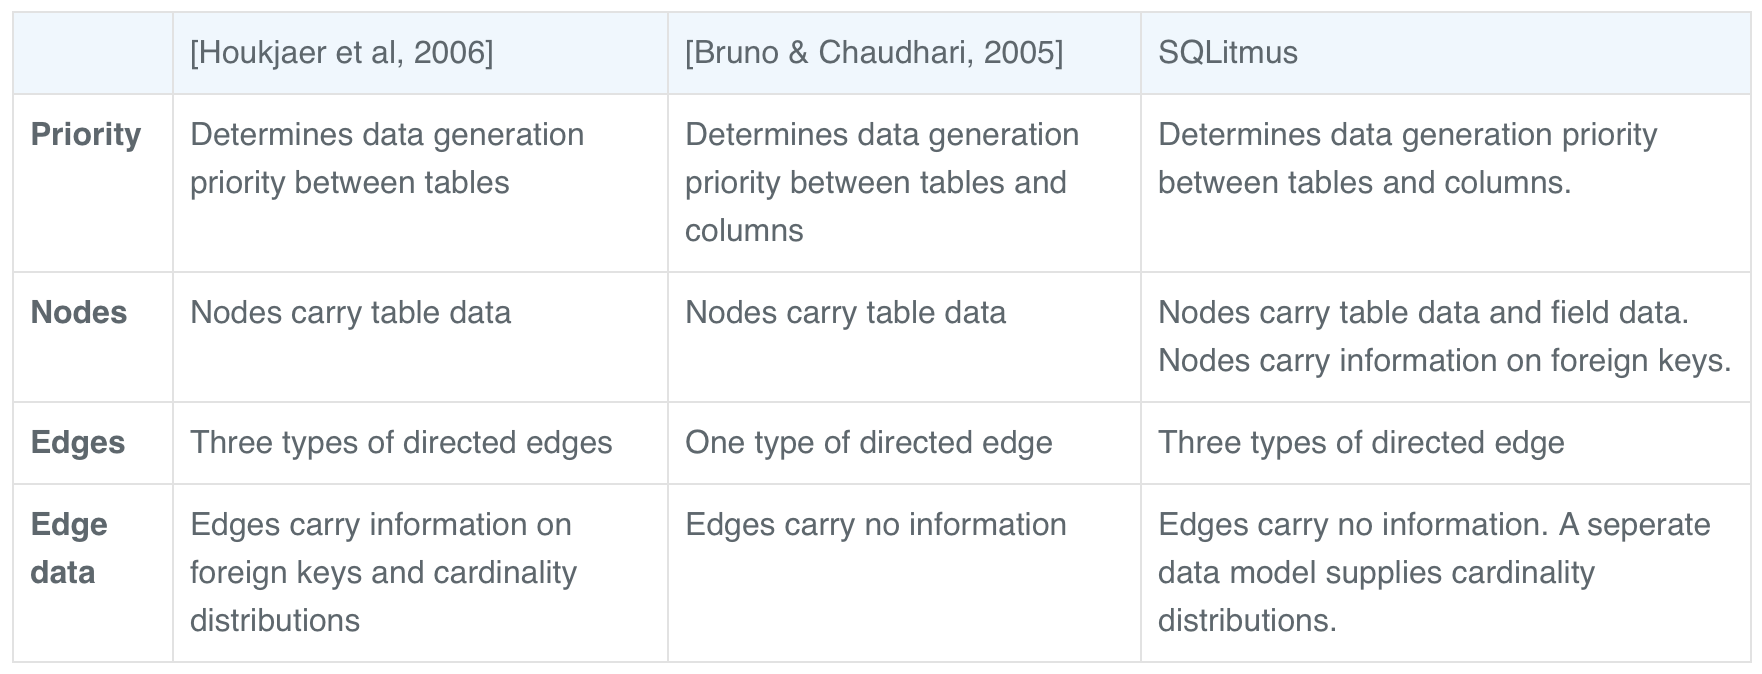
\includegraphics[width=\textwidth]{2-3-1.png}
			\caption{Table of graph models}
			
		\end{figure}
		
		
		\textbf{Priority:} Like Bruno’s\cite{Bruno:2005} model, SQLitmus’s graph model is capable of determining the order of data generation between tables and columns. While SQLitmus’s graph model is capable of supporting intra-row data dependencies, the feature has been excluded - since offering intra-row dependencies necessarily clutters the GUI, forces developers to make additional configurations, and slows down the data generation process. The graph model is currently used to specify the data generation order between tables, and to delay the generation of self-referential foreign keys. Self-referential foreign keys must necessarily be generated after the column of the same table that it references.
		
		\textbf{Nodes:} Nodes in SQLitmus stores referential constraints on a field level which are then parsed to generate referential constraints on a table level. Storing referential constraints on a field level allows SQLitmus to generate self-referential foreign keys and composite foreign keys with more ease.
		
		\textbf{Edges:} Like Houkjaer’s model, SQLitmus’s graph model supports Normal, Forward, and Backward edges. Simple and composite primary and foreign keys are supported. Only simple self-referential foreign keys are supported.
		
		
		\subsubsection{Query generation implications}
		On the query generation front, SQLitmus employs a similar methodology as QGEN\cite{Poess:2004}. It also uses a combination of query templates and a query preprocessor to generate random queries of high quality. In fact, SQLitmus’s query generator arguably generates random queries of higher quality as compared to the query templating function employed by QGEN. It requires no additional configurations as it simply uses the exact same set of data generators already configured for use by the test data generator. SQLitmus’s templating options are also much more robust and flexible as compared to those available in QGEN. It provides functionality that addresses the two critical flaws of QGEN’s query generation technique discussed in (Subsection 2.2). It is able to guarantee that every SELECT, INSERT, UPDATE, and DELETE query affects at least one row of available data when used correctly. It is also able to reverse the impact of single-row INSERT and DELETE statements and ensure that the cardinality of the data-set does not drift off too much as test queries are being executed. Its only critical flaw is that it is currently unable to reverse the impact of bulk delete statements.
		
		Techniques to ensure zero cardinality drift\footnote{The phenomenon where the tested queries modify the cardinality of the data-set through INSERT or DELETE statements. If unaccounted for, results in unreliable performance analyses. } of the test data-set, while not implemented, have been devised, and will be presented in (Subsection 6.2).
		
		\subsubsection{Random Number Generator (RNG)}
		
		To generated deterministic random sets of data across multiple test sessions and databases, SQLitmus relies on the PCG-XSH-RR RNG introduced by O'Neill \cite{oneill:pcg2014}. The above-mentioned RNG belongs to the permuted congruential generator (PCG) family of random number generators. The RNG was selected for the following properties:
		\begin{itemize}
			\item Seeded - Allows for identical RNG sequences to be generated across different runs.
			\item Fast - Generates the next state at a very low constant cost
			\item Logarithmic random access - Able to jump ahead to the $n^{th}$ number in the RNG sequence in $log(n)$ time.
			\item High periodicity - A period of $2^n$ where n is the number of bits used to store the state.
			\item High uniformity - At any point of the random number generation process, generated numbers occur at highly uniform frequencies across the range.
		\end{itemize}
		
		
		SQLitmus employs a 64-bit implementation of the RNG which is has a period of $2^{64}$, much higher than the current data size generation limit that SQLitmus supports. The fast logarithmic random access times when used in conjunction with the PDGF seeding strategy proposed by \cite{Rabl:2010} and \cite{Alexandrov:2012} will enable SQLitmus to generate data with intra-row, inter-column, and inter-table dependencies without performing expensive disk reads. This feature while impressive, requires a fair bit of effort to implement, and is thus de-priotized to a later patch.
		
		SQLitmus also utilizes a good multiplier constant proposed by \cite{LEcuyer:1999} to ensure a high uniformity in randomly generated numbers. A poorly chosen multiplier constant will also reduce the period of the RNG. 
		
		
		\subsection{Trade Offs}
		
		\begin{figure}[H]
			\centering
			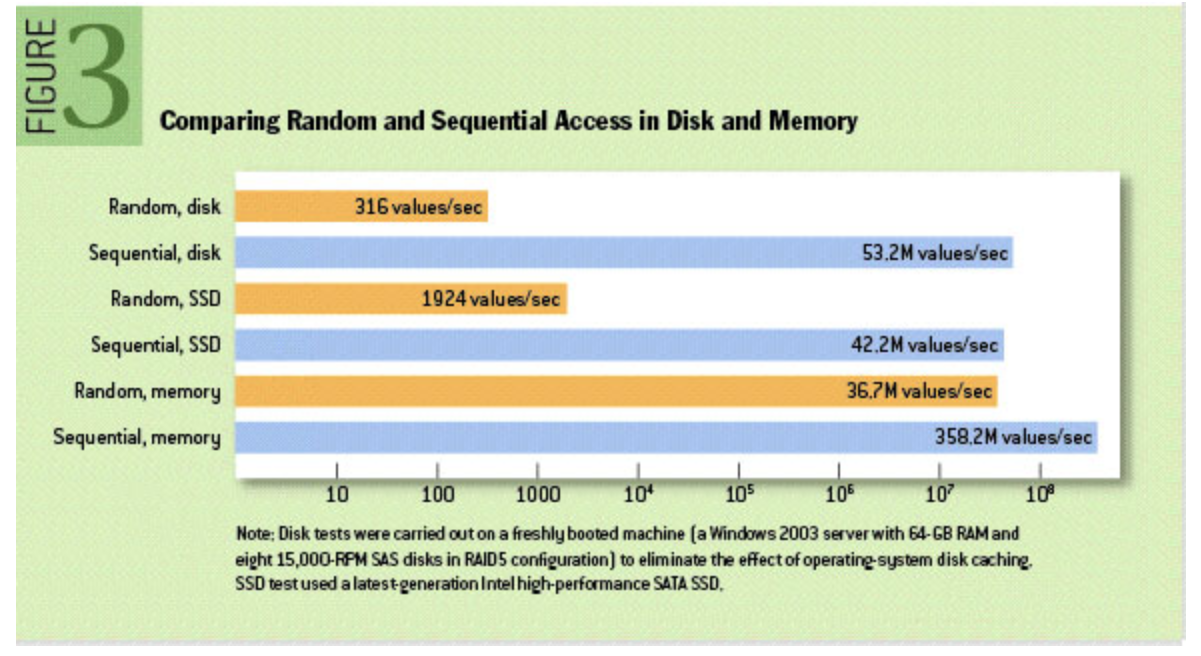
\includegraphics[width=\textwidth]{2-3-4.png}
			\caption{Performance of RAM, SSD, and HDD \cite{Jacobs:2009}}
			
		\end{figure}
		
		
		For each test, SQLitmus is only able to generate data up to the the amount of RAM available on the client-side computer. This is because SQLitmus stores the entire data-set in memory. This trade-off is made for the following reasons:
		\begin{itemize}
			\item While SQLitmus generates and is capable of storing data sequentially, the database currently used to manage the data generation process, NeDB, only allows random access updates. 
			\item Data generation will be approximately 1,000,000 times faster on RAM vs HDD
			\item Data generation will be approximately 200,000 times faster on RAM vs SSD
			\item There is no need to persist the data generated by SQLitmus (It is already on a database)
			\item Developers of small-to-medium sized applications rarely store more than 10GB of data
			\item Large binary objects such as flat files and pictures are usually stored in the server.
		\end{itemize}
		
		
		To reiterate, the key goal of SQLitmus is to to make database performance testing fast, convenient, accessible, and reliable. Initial trade-offs were made in favour of speed as opposed to the maximal data-set size. As the author believes that an approximate 10 GB limit is sufficient for most developers using the tool. SQLitmus currently takes approximately a minute to generate 1,000,000 fields of data. Thus, storing the data-set on-disk at this moment would be untenable.
		
		Nonetheless, SQLitmus is intending to rework its data generation process to off-load most of the in-memory data storage to disk (Since transferring a random access load in-memory to a sequential load on-disk actually provides a performance benefit). If this effort is successful, SQLitmus will be able to generate data at an almost constant speed while requiring that only a fraction of the data-set currently being generated resides in memory. This future work will be discussed in (Section 6.2).
		
		
		\section{SQLitmus Features}
		
		Every good software begins by serving the needs of its target users well. This section begins by enunciating the user stories that developers of small-to-medium sized applications want from SQL database performance analysis tools. 
		
		As a user, I want...
		\begin{itemize}
			
			\item A performance test that is reliable, so that I am sure that the performance testing is accurate.
			\item A performance test that is repeatable, so that I am able to test for the impacts of the new configurations I made.
			\item A performance test that is repeatable, so that I am able to select the most suitable database system to use.
			\item A way to save my configurations, so that I do not have to waste time reconfiguring my tests.
			\item An easy and convenient way of testing my SQL databases, so that I can focus my efforts on developing my software.
			\item A good way of visualizing my performance testing data, so that I do not have to waste time exporting them into another software.
			\item A way to test my database's performance under multiple configurations, so that I can identify performance bottlenecks and trends more effectively. 
			\item A way to test my database under different data loads, so that I have a sense of how well my database scales with an increasing data load.
			\item A way to test my database under different numbers of concurrent connections, so that I have a sense of how well my database scales with an increasing number of concurrent users.
			\item A way to test my database with multiple types of queries, so that I have a more complete understanding of my database's performance.
			\item A way to specify the types of data I wish to generate, so that I can ensure that they are compliant with my database schema.
			\item A way to specify the types of queries I wish to test, so that the test results are more representative of my software's actual performance.
			\item A software that guides me through the configuration process, so that I do not have to spend time figuring it out.
			\item A way to test my database quickly, so that I do not have to wait too long to see the results of my test.
		\end{itemize}
		With the user stories enunciated, the remainder of this section demonstrates how SQLitmus's feature set provides a solution for all of the above-mentioned user stories.
		
		Note that the feature set in this section is often explained through the use of the test scenario presented in (Section 4). While this section is designed to be self-sufficient, readers may opt to refer to the test design in (Section 4) to gain a clearer understanding of the specific scenario used. For readers who are unfamiliar with how SQL databases operate, the author recommends reading (Section 4) first.
		
		
		\subsection{Database Connection Management}
		
		
		\begin{figure}[H]
			\centering
			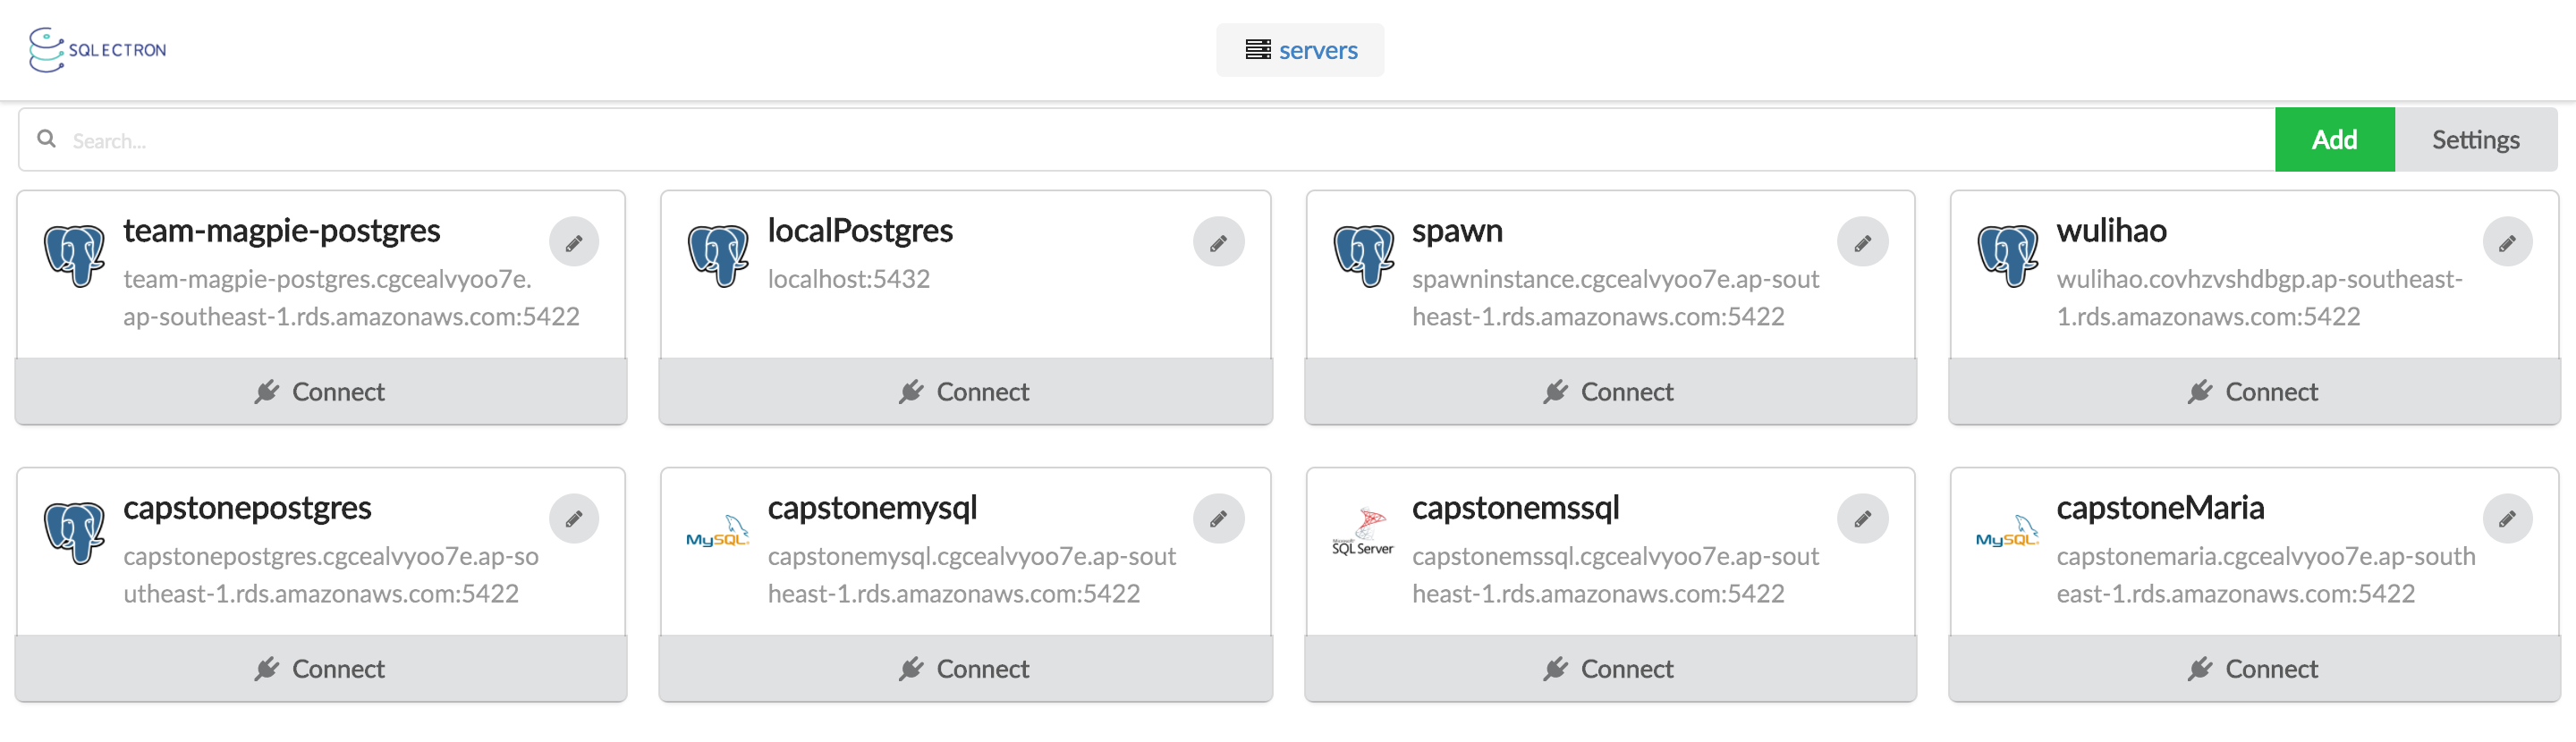
\includegraphics[width=\textwidth]{3-1.png}
			\caption{SQLitmus landing page }
			
		\end{figure}
		
		SQLitmus's landing page (see Figure 3) offers a way for developers to manage and persist their database connection configurations. Developers are able to add a new set of connection settings, or update their existing set of connection settings. The database management dashboard was forked off the open-source tool SQLectron which already provided a user-friendly GUI for database connection management. Beyond persisting database connection settings, SQLectron does not support any further types of persistence.
		
		To afford developers an additional layer of convenience, SQLitmus persists all available configurations discussed in later sections on a database level. This prevents configurations made for a particular database to spillover into other databases even when they belong to the same server.
		
		\subsection{Data Generation}
		
		
		\begin{figure}[H]
			\centering
			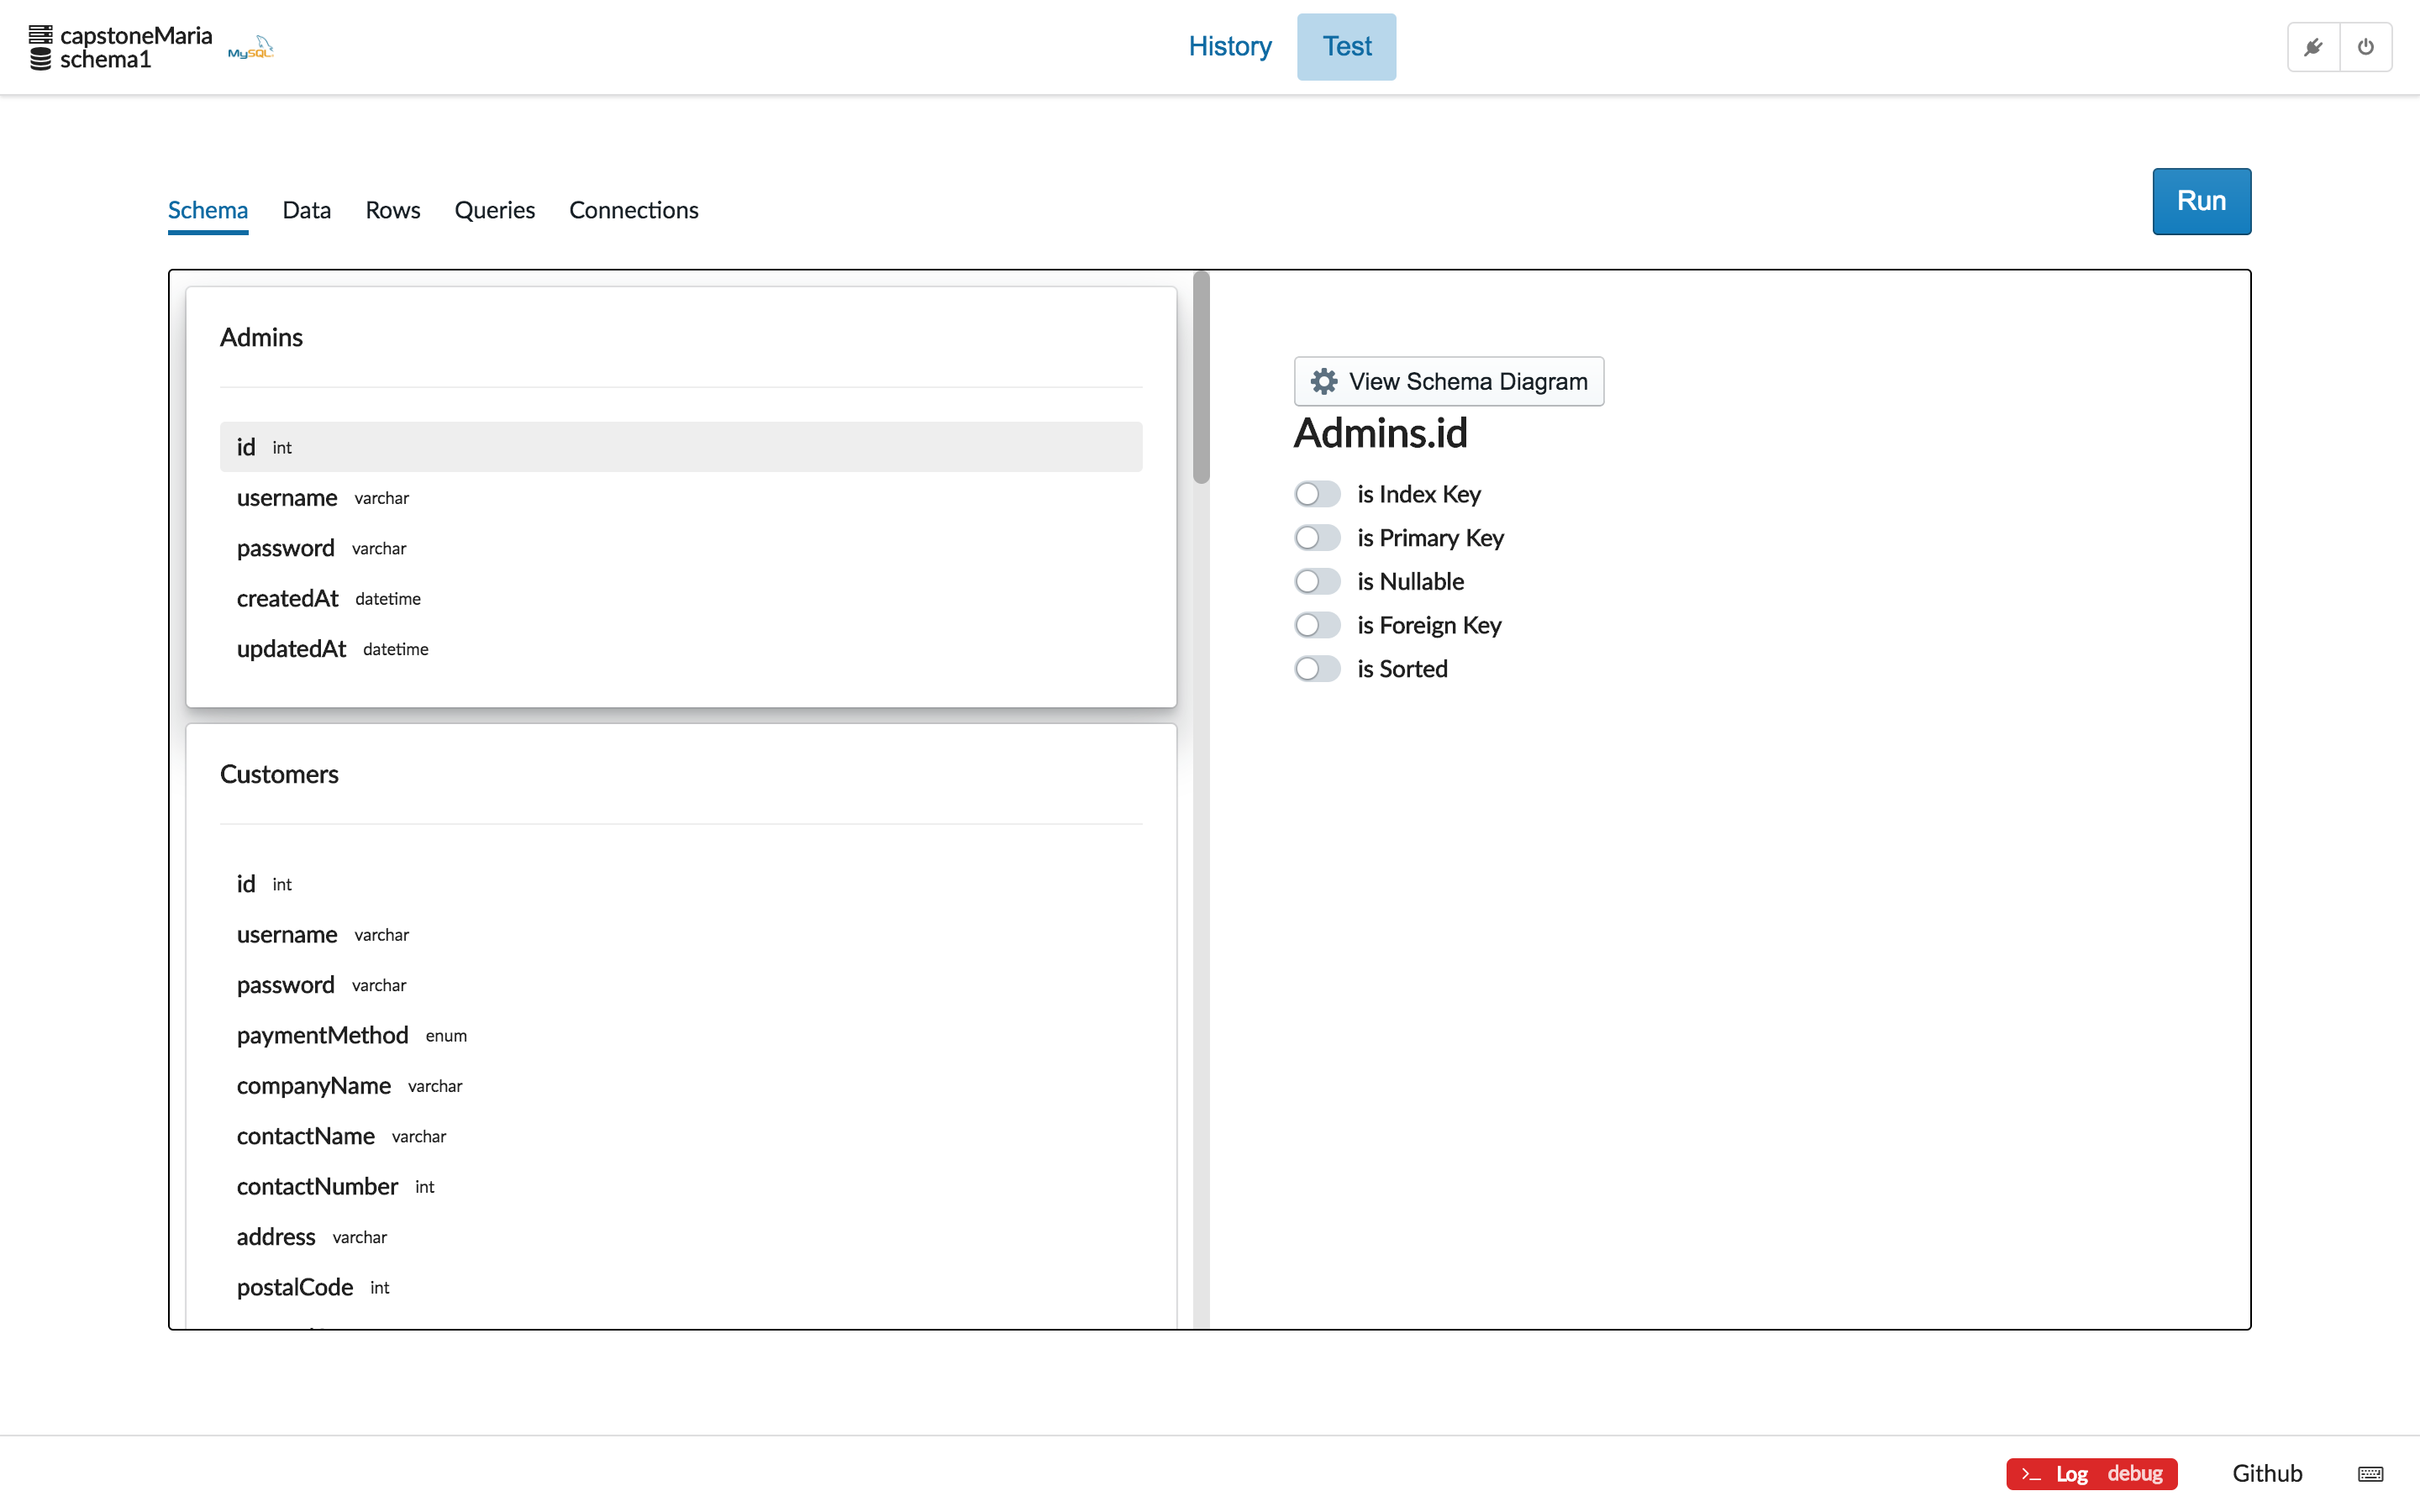
\includegraphics[width=\textwidth]{3-2.png}
			\caption{SQLitmus automatically populating tables and fields}
			
		\end{figure}
		
		Upon connecting to a specified database, SQLitmus populates the the GUI with the full list of tables and fields present on the database (excluding system databases). Field types are also auto-populated.
		
		Figure 4 displays how the SQLitmus GUI looks like upon connecting to a database for the first time. Without any configuration, relevant details of a database's schema is populated by default into SQLitmus.
		
		\subsubsection{ Configuring field constraints}
		
		
		\begin{figure}[H]
			\centering
			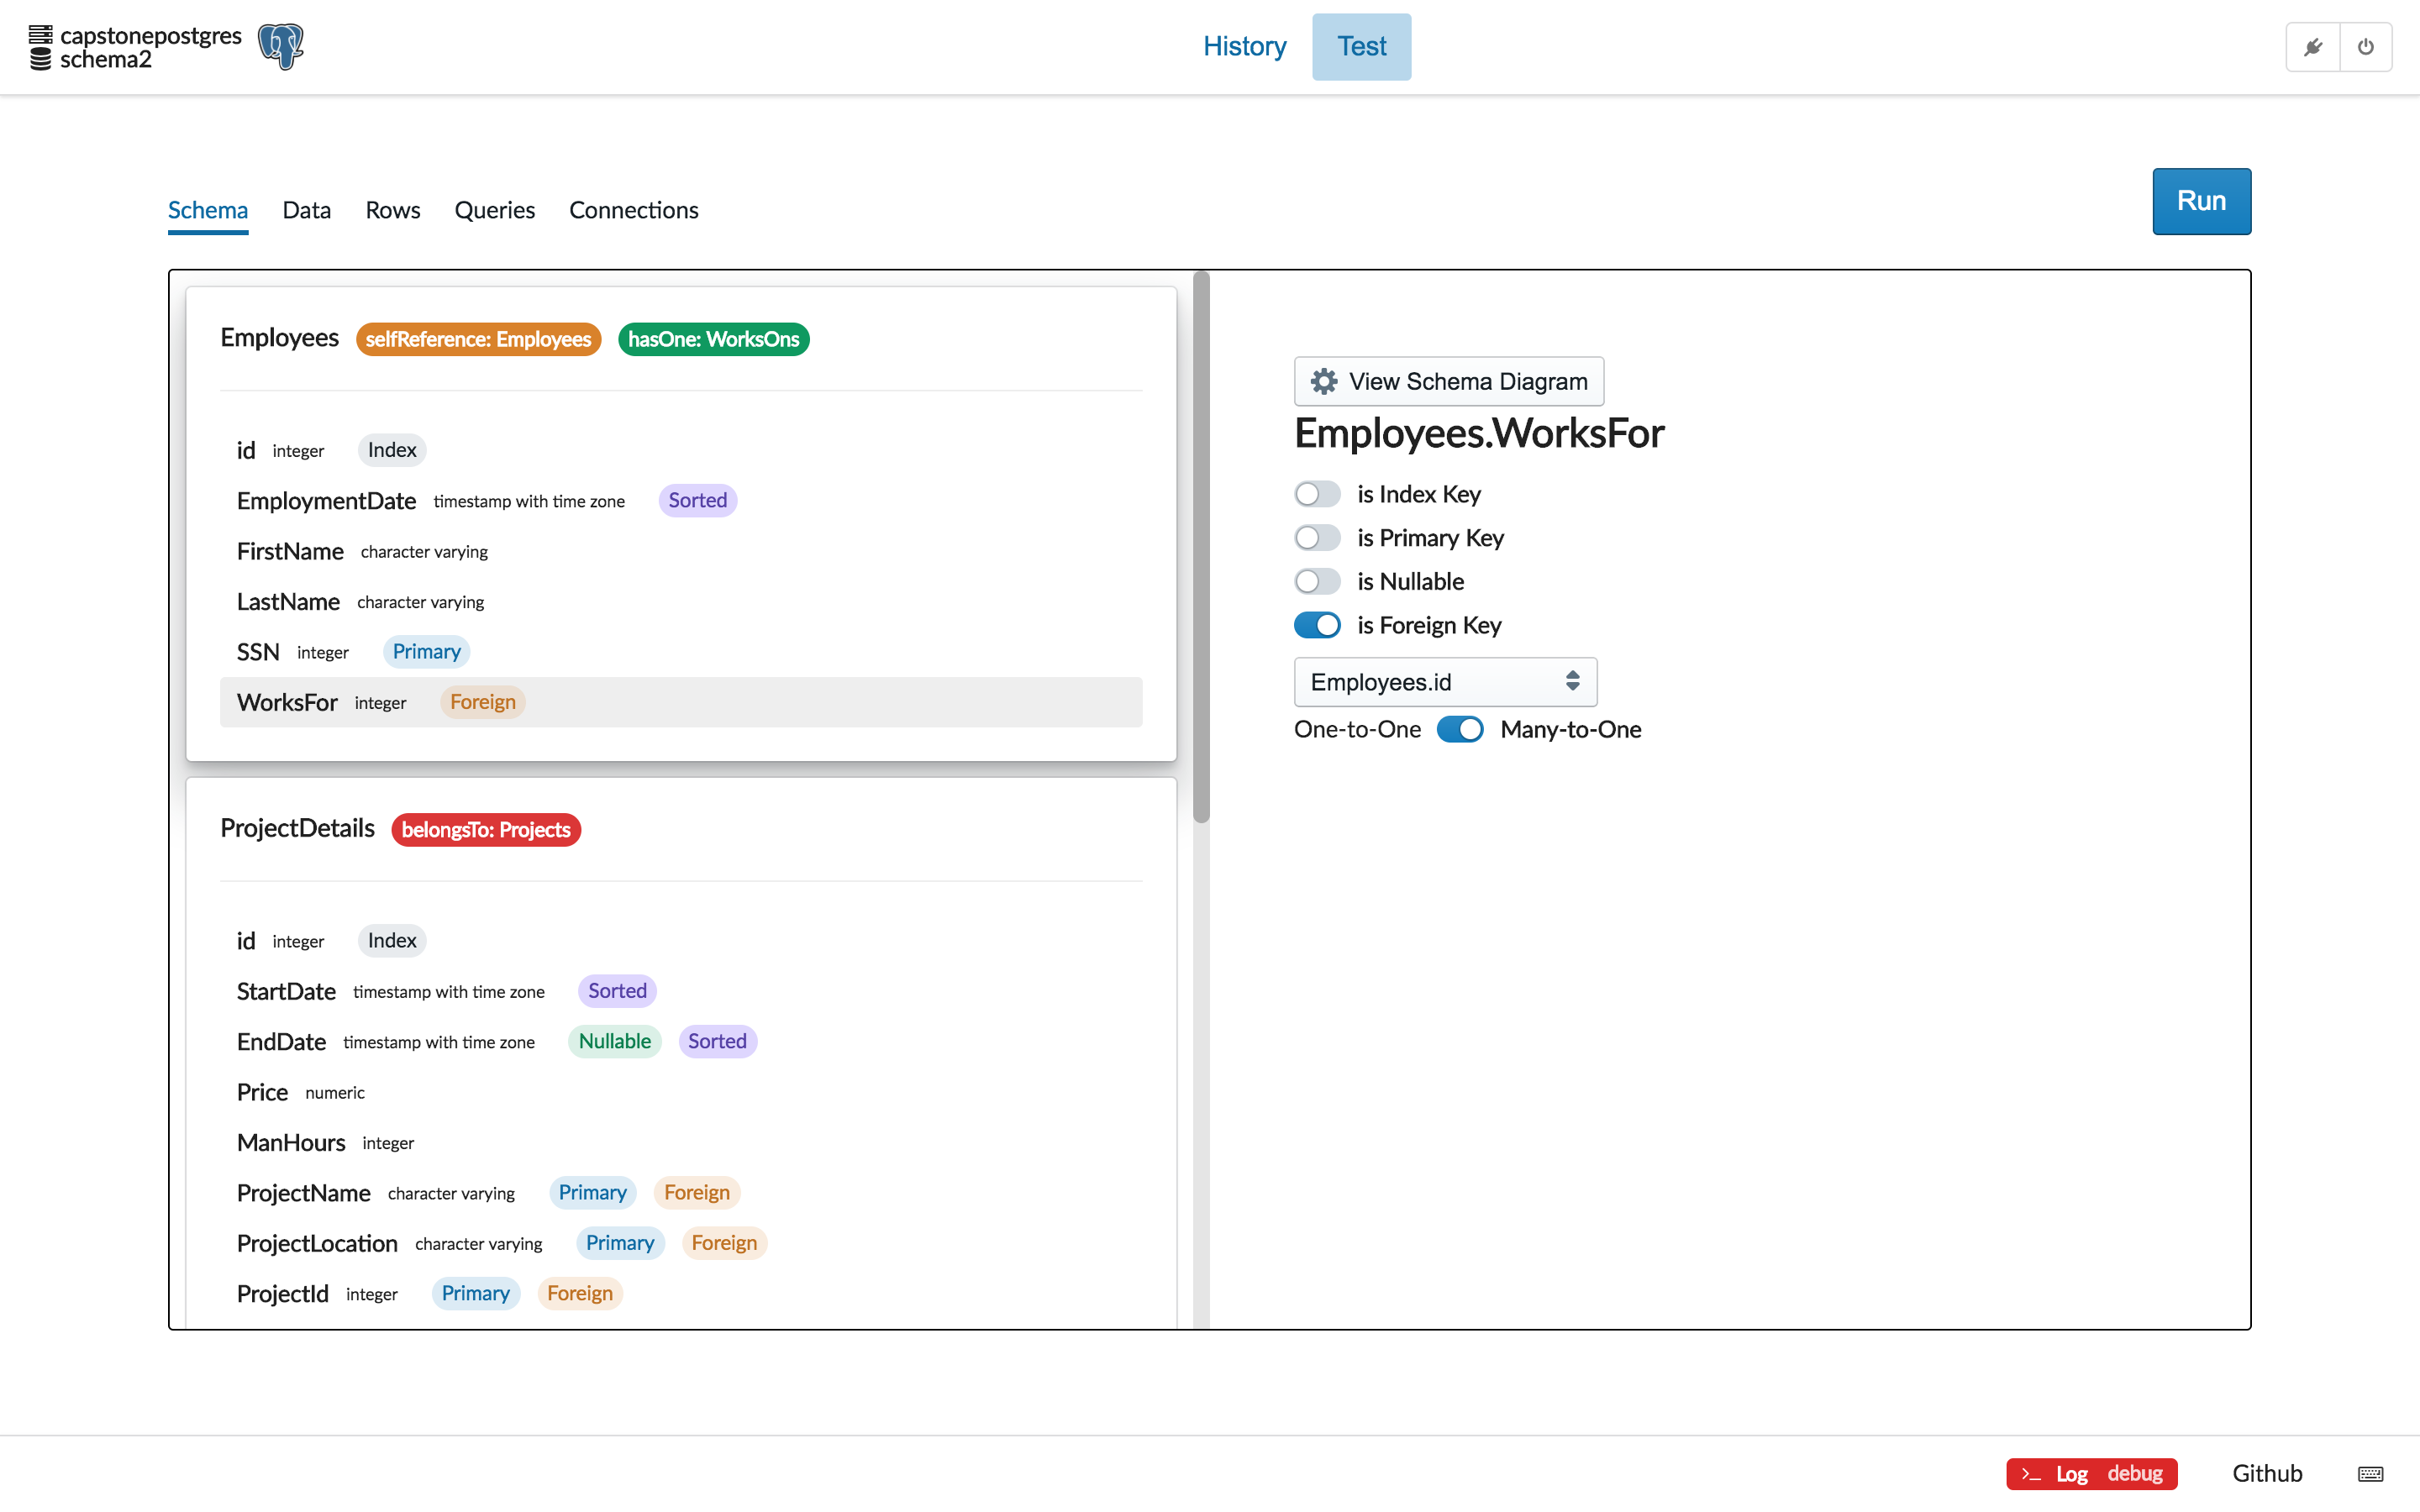
\includegraphics[width=\textwidth]{3-2-1.png}
			\caption{Field constraint configurations }
			
		\end{figure}
		
		SQLitmus supports six different forms of field constraints\footnote{Specifies the rules that fields in a SQL database has to comply with}: Index Key\footnote{An integer field that is guaranteed to be unique down a column}, Primary Key\footnote{A single or combination of multiple fields that guarantees a record's uniqueness}, Nullable\footnote{A field that is allowed to hold null values}, Foreign Key\footnote{A single or combination of multiple fields that guarantees a unique record is referenced.}, Unique Key\footnote{A field that is guaranteed to be unique down a column}, and Sorted\footnote{A field that is guaranteed to be sorted down a column} constraints.
		
		As users configure field constraints, the GUI provides clear visual feedback. This is demonstrated in Figure 5, where field constraints appear as tags next to their relevant fields and foreign key constraints appear as tags next to their relevant tables.
		
		Developers are able to specify their field constraints though simple switches and selections. No text or numerical inputs are offered. This achieves a twofold purpose: simplify the configuration process, and eliminate the risk of misconfiguration altogether. 
		
		
		
		
		\begin{figure}[H]
			\centering
			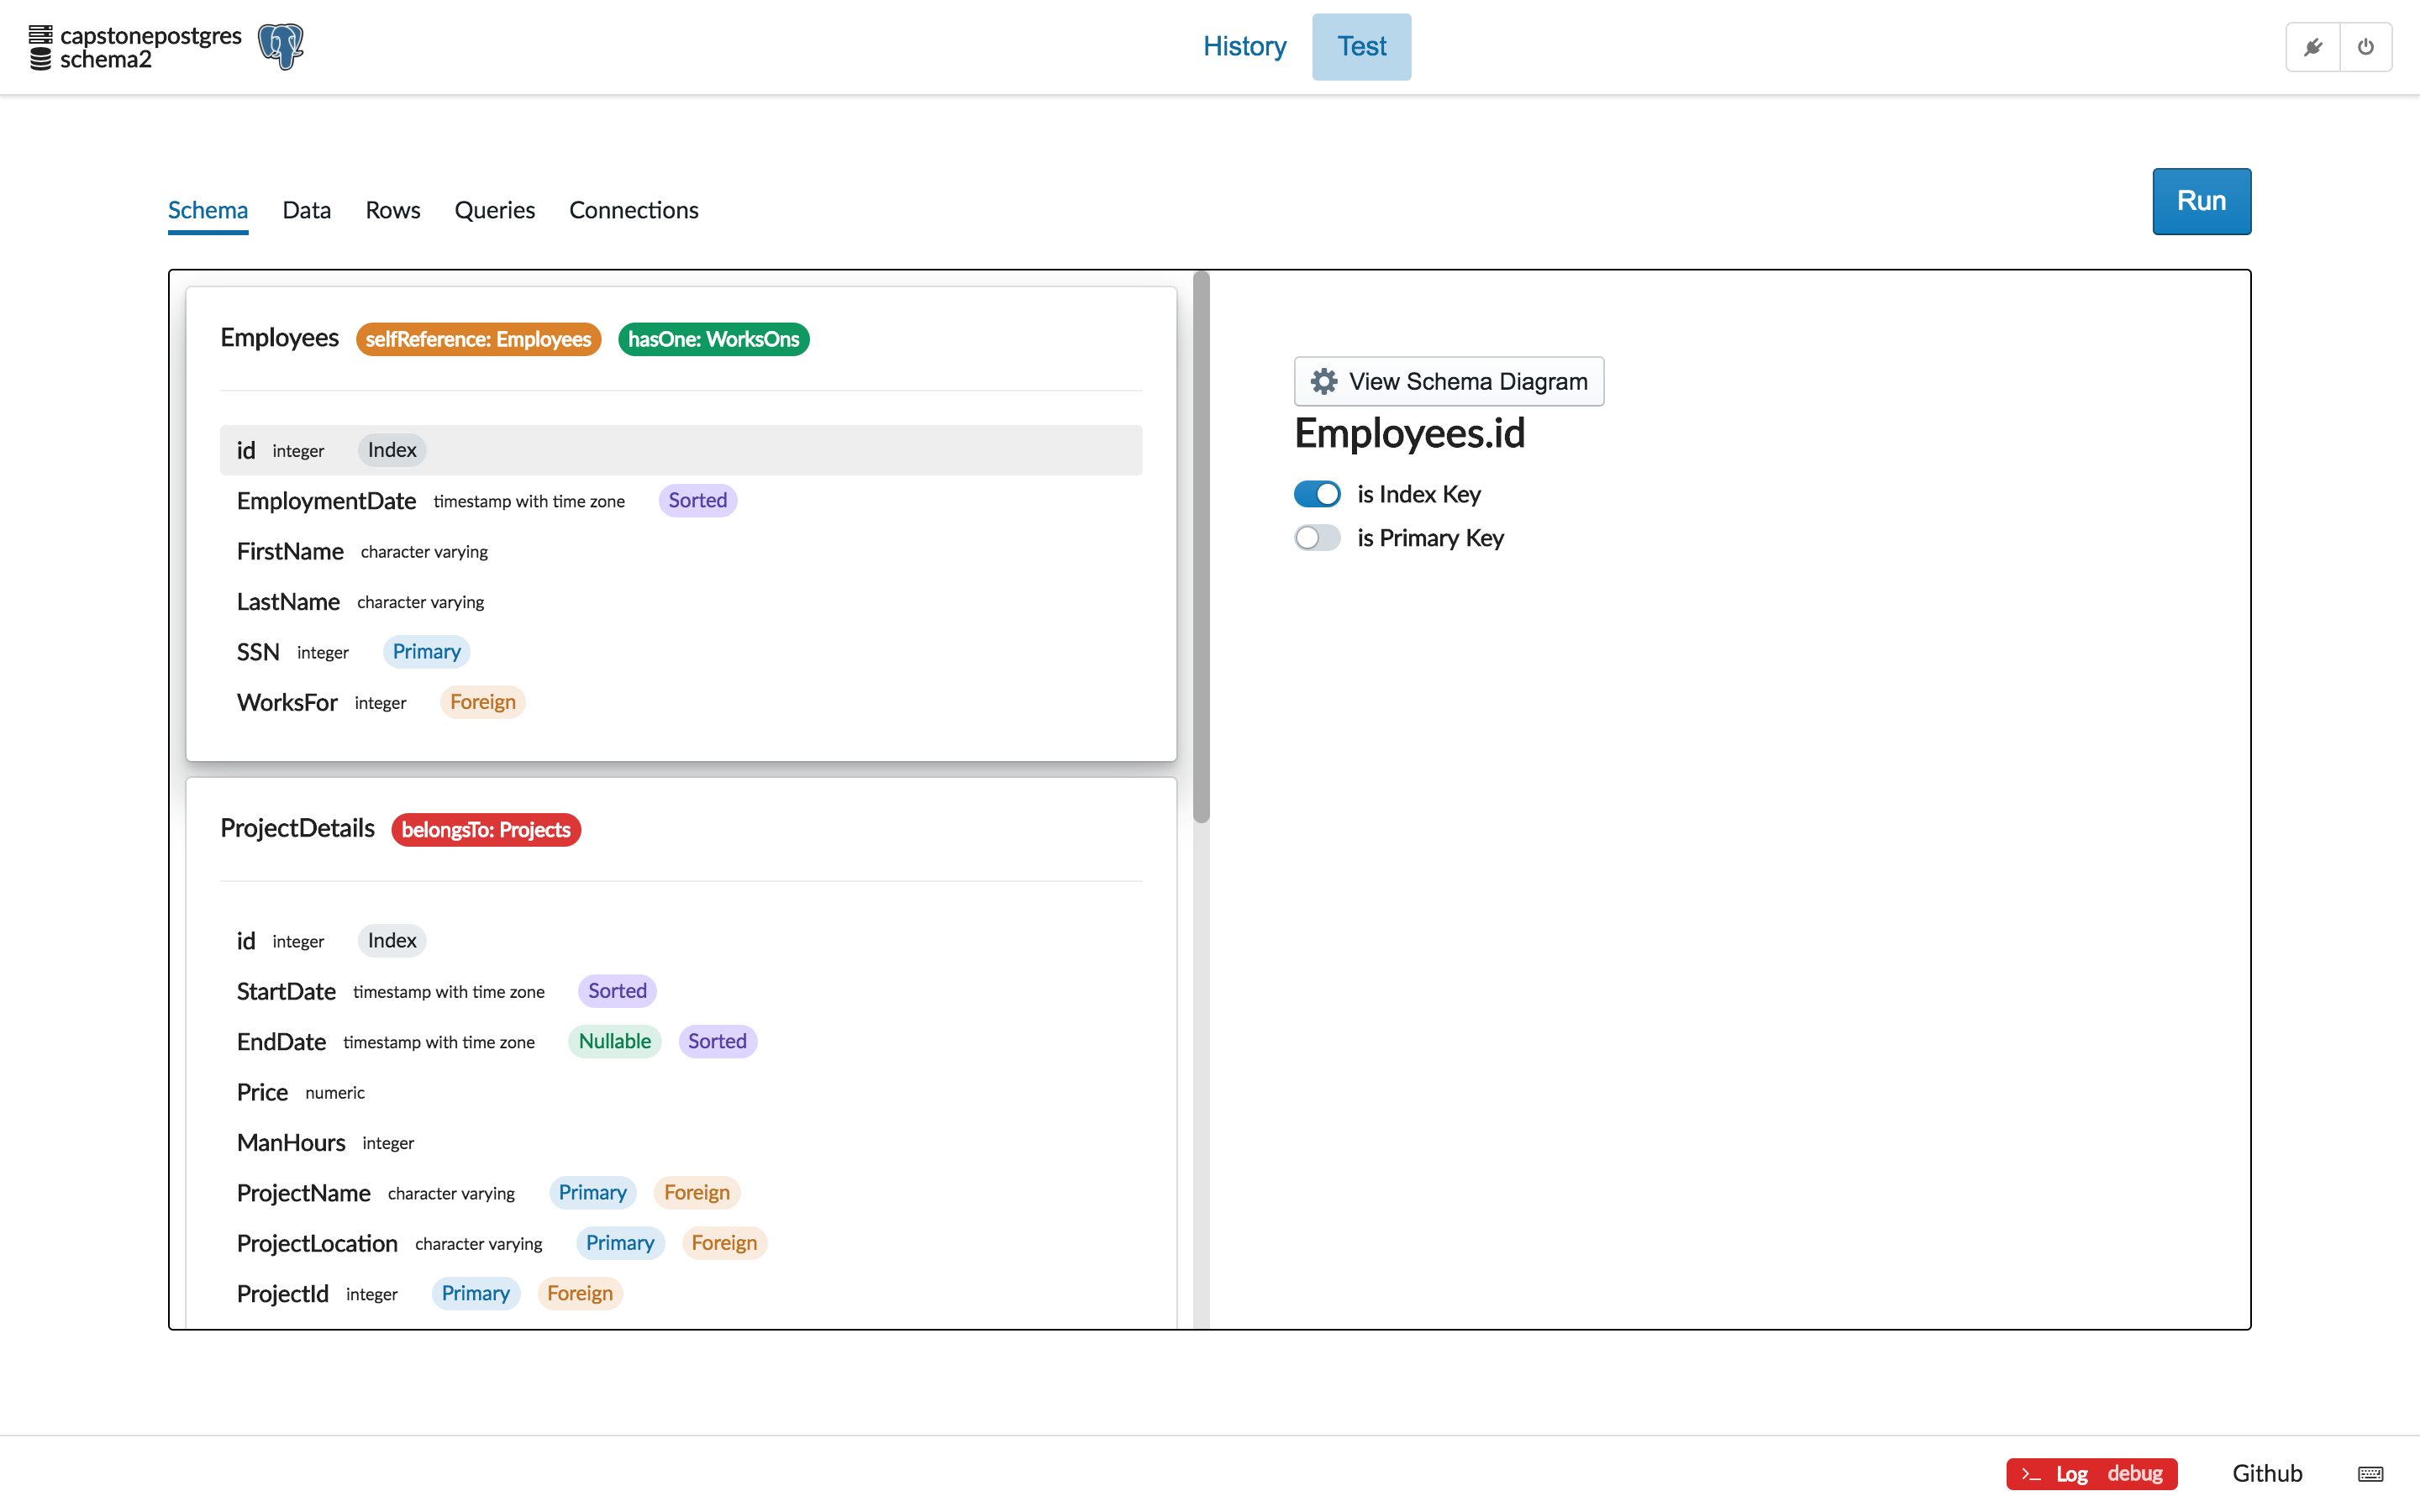
\includegraphics[width=\textwidth]{3-2-1b.png}
			\caption{Selecting upstream constraints disable invalid downstream configurations}
			
		\end{figure}
		
		As developers specify upstream constraints, invalid downstream configurations are disabled.
		
		This behavior is observed in figure 6 where configuring an index field disables developers from specifying other invalid downstream configurations. The rationale is as follows - index fields necessarily cannot be foreign keys, or nullable fields. It is also taken for granted that index fields are unique and sorted.
		
		SQLitmus also limits developers from specifying configurations that are disallowed by databases (eg. specifying an index key on a non-integer field), considered anti-patterns in the developer community (eg. using timestamps as primary or foreign keys), or breaks referential integrity (eg. selecting a non index, primary, or unique key as a foreign key target). 
		
		
		\begin{figure}[H]
			\centering
			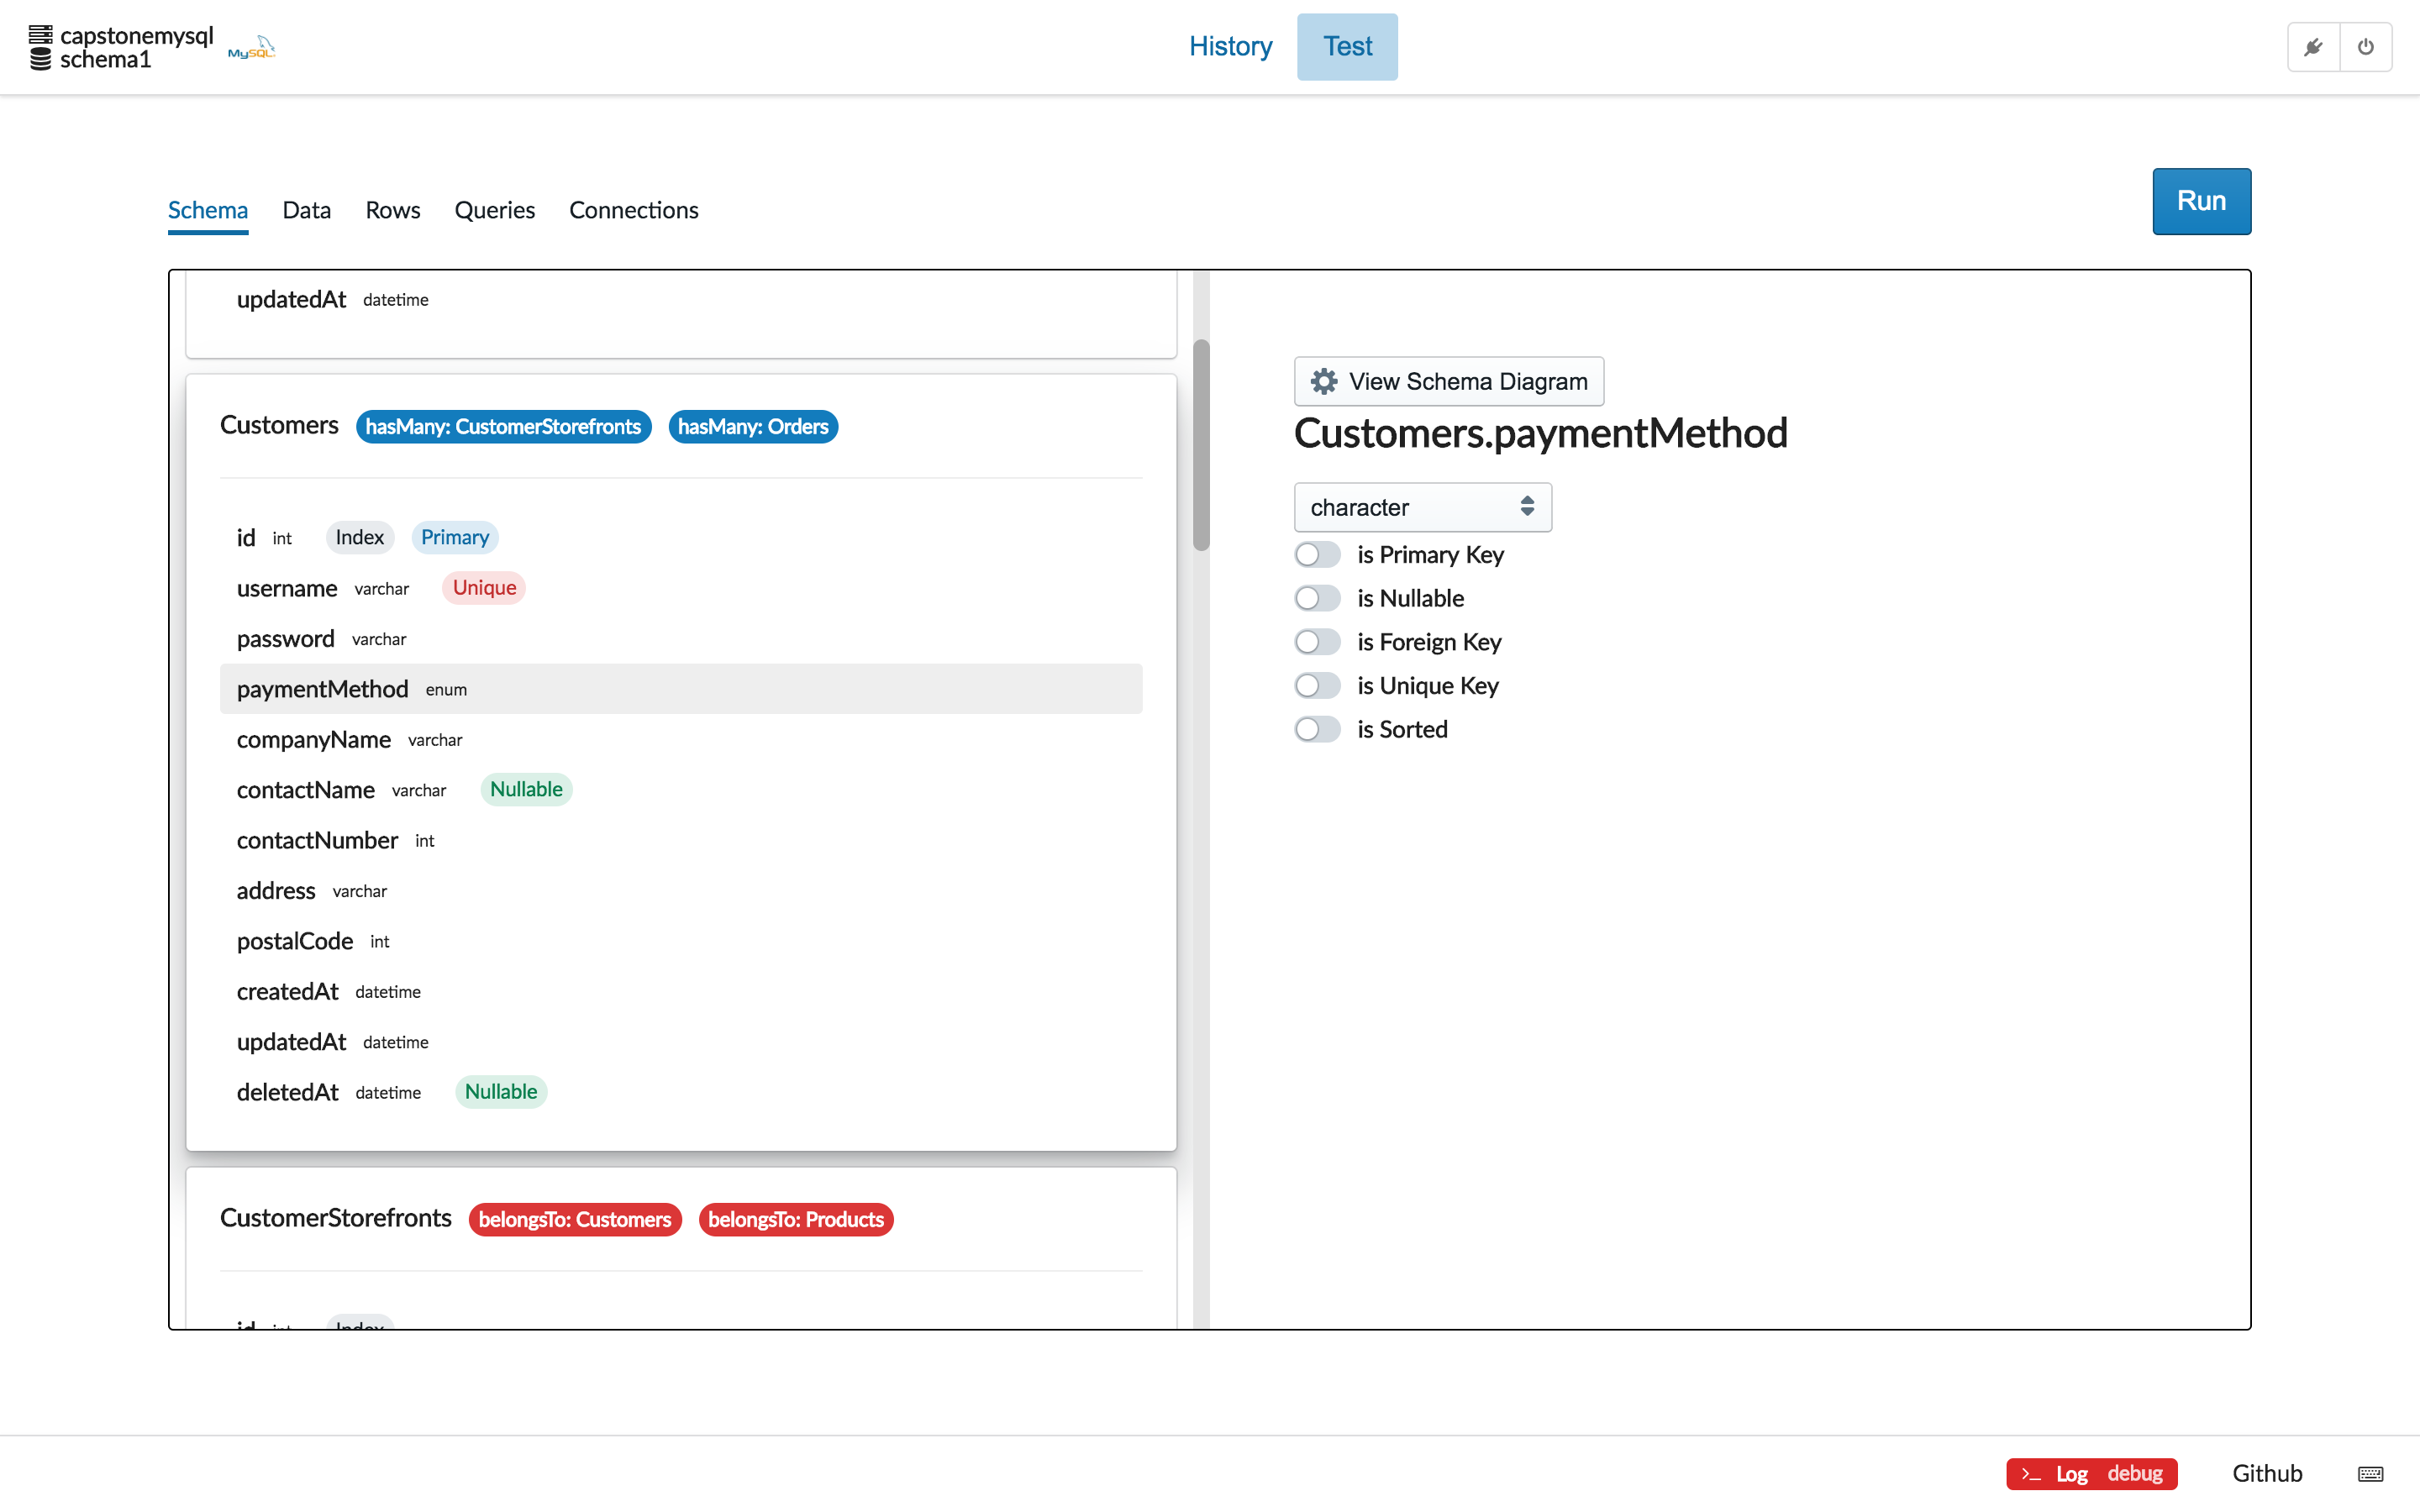
\includegraphics[width=\textwidth]{3-2-1c.png}
			\caption{Unsupported data type configuration}
			
		\end{figure}
		
		For unsupported data types, SQLitmus allows developers to configure the field type according to one of the six supported types: integer, character, numeric, boolean, time, json. For all downstream configurations, SQLitmus will treat the unsupported type as the type configured by the developer. Figure 7 demonstrates how unsupported data types can be configured into one of SQLitmus's supported types.
		
		
		
		
		\begin{figure}[H]
			\centering
			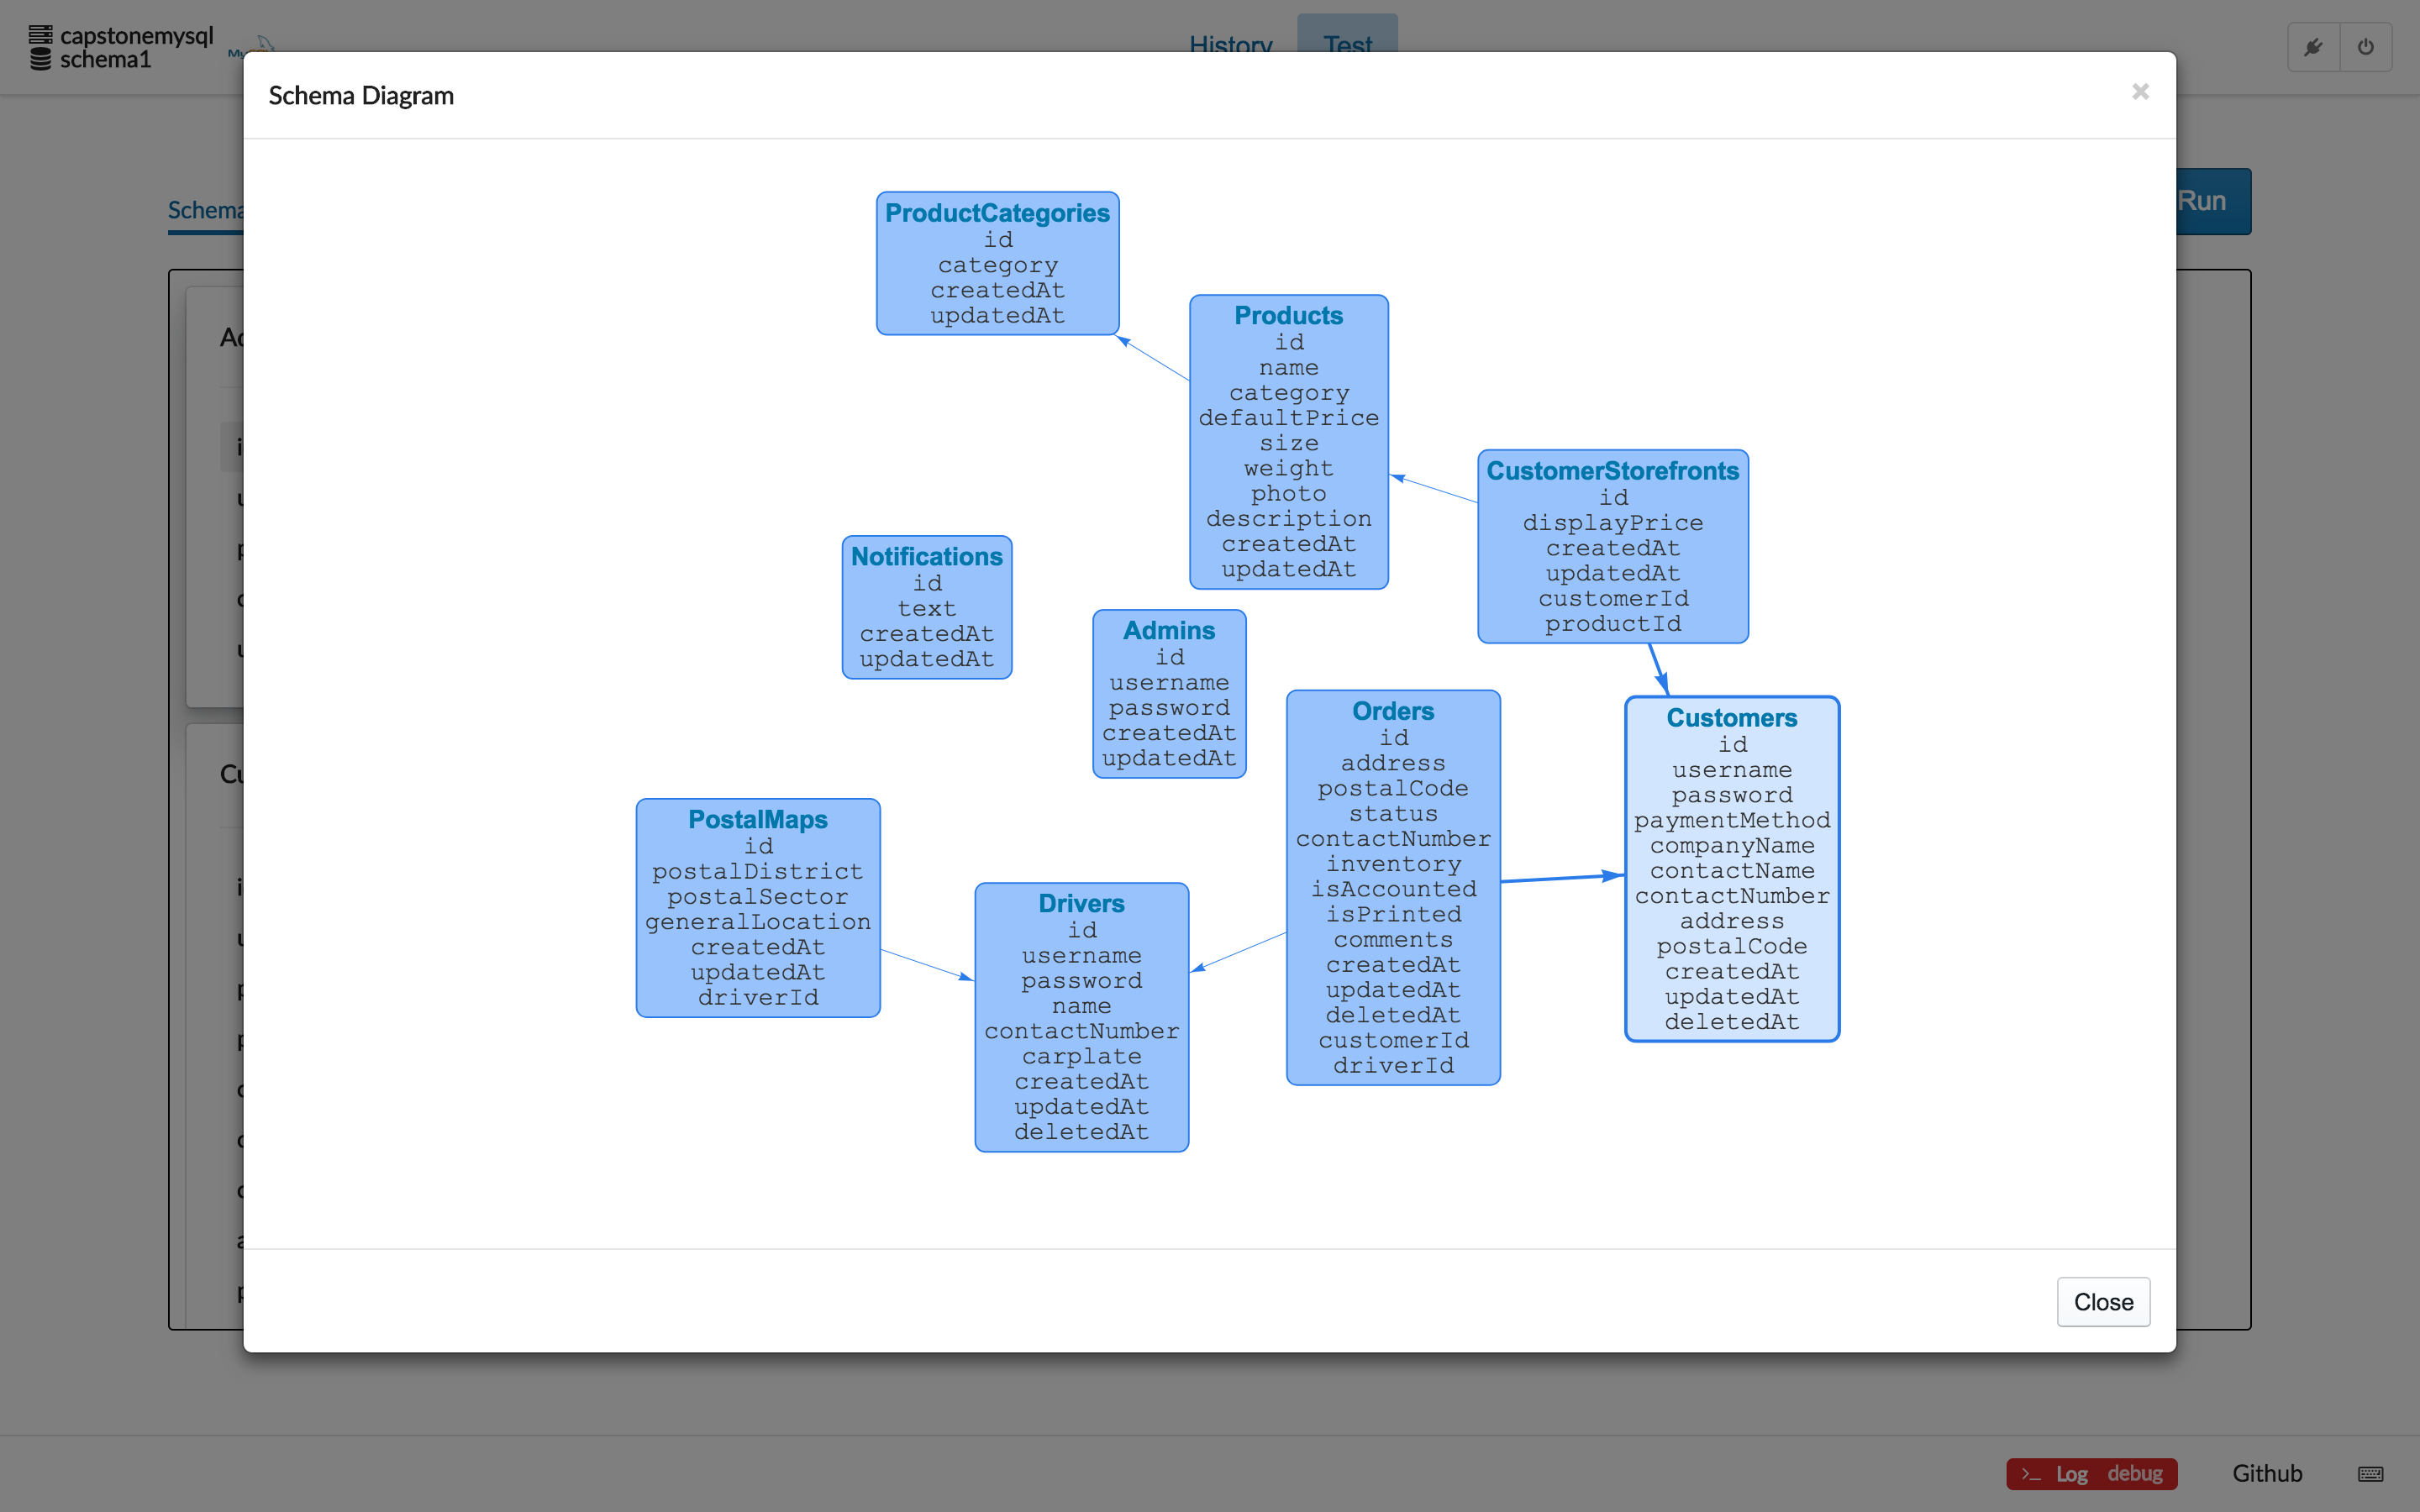
\includegraphics[width=\textwidth]{3-2-1d.png}
			\caption{Visualization of schema diagram }
			
		\end{figure}
		
		Developers are also able to view a diagram of their schema to quickly identify misconfigured foreign key relations. Figure 8 demonstrates one such diagram.
		
		\subsubsection{Configuring Data Generators}
		
		While data generators can be configured at any point of the configuration process, the author recommensd that data generator configurations are performed after field constraints configurations. This allows for a smoother configuration process as some data generators may be invalidated by changes in field constraints.
		
		
		\begin{figure}[H]
			\centering
			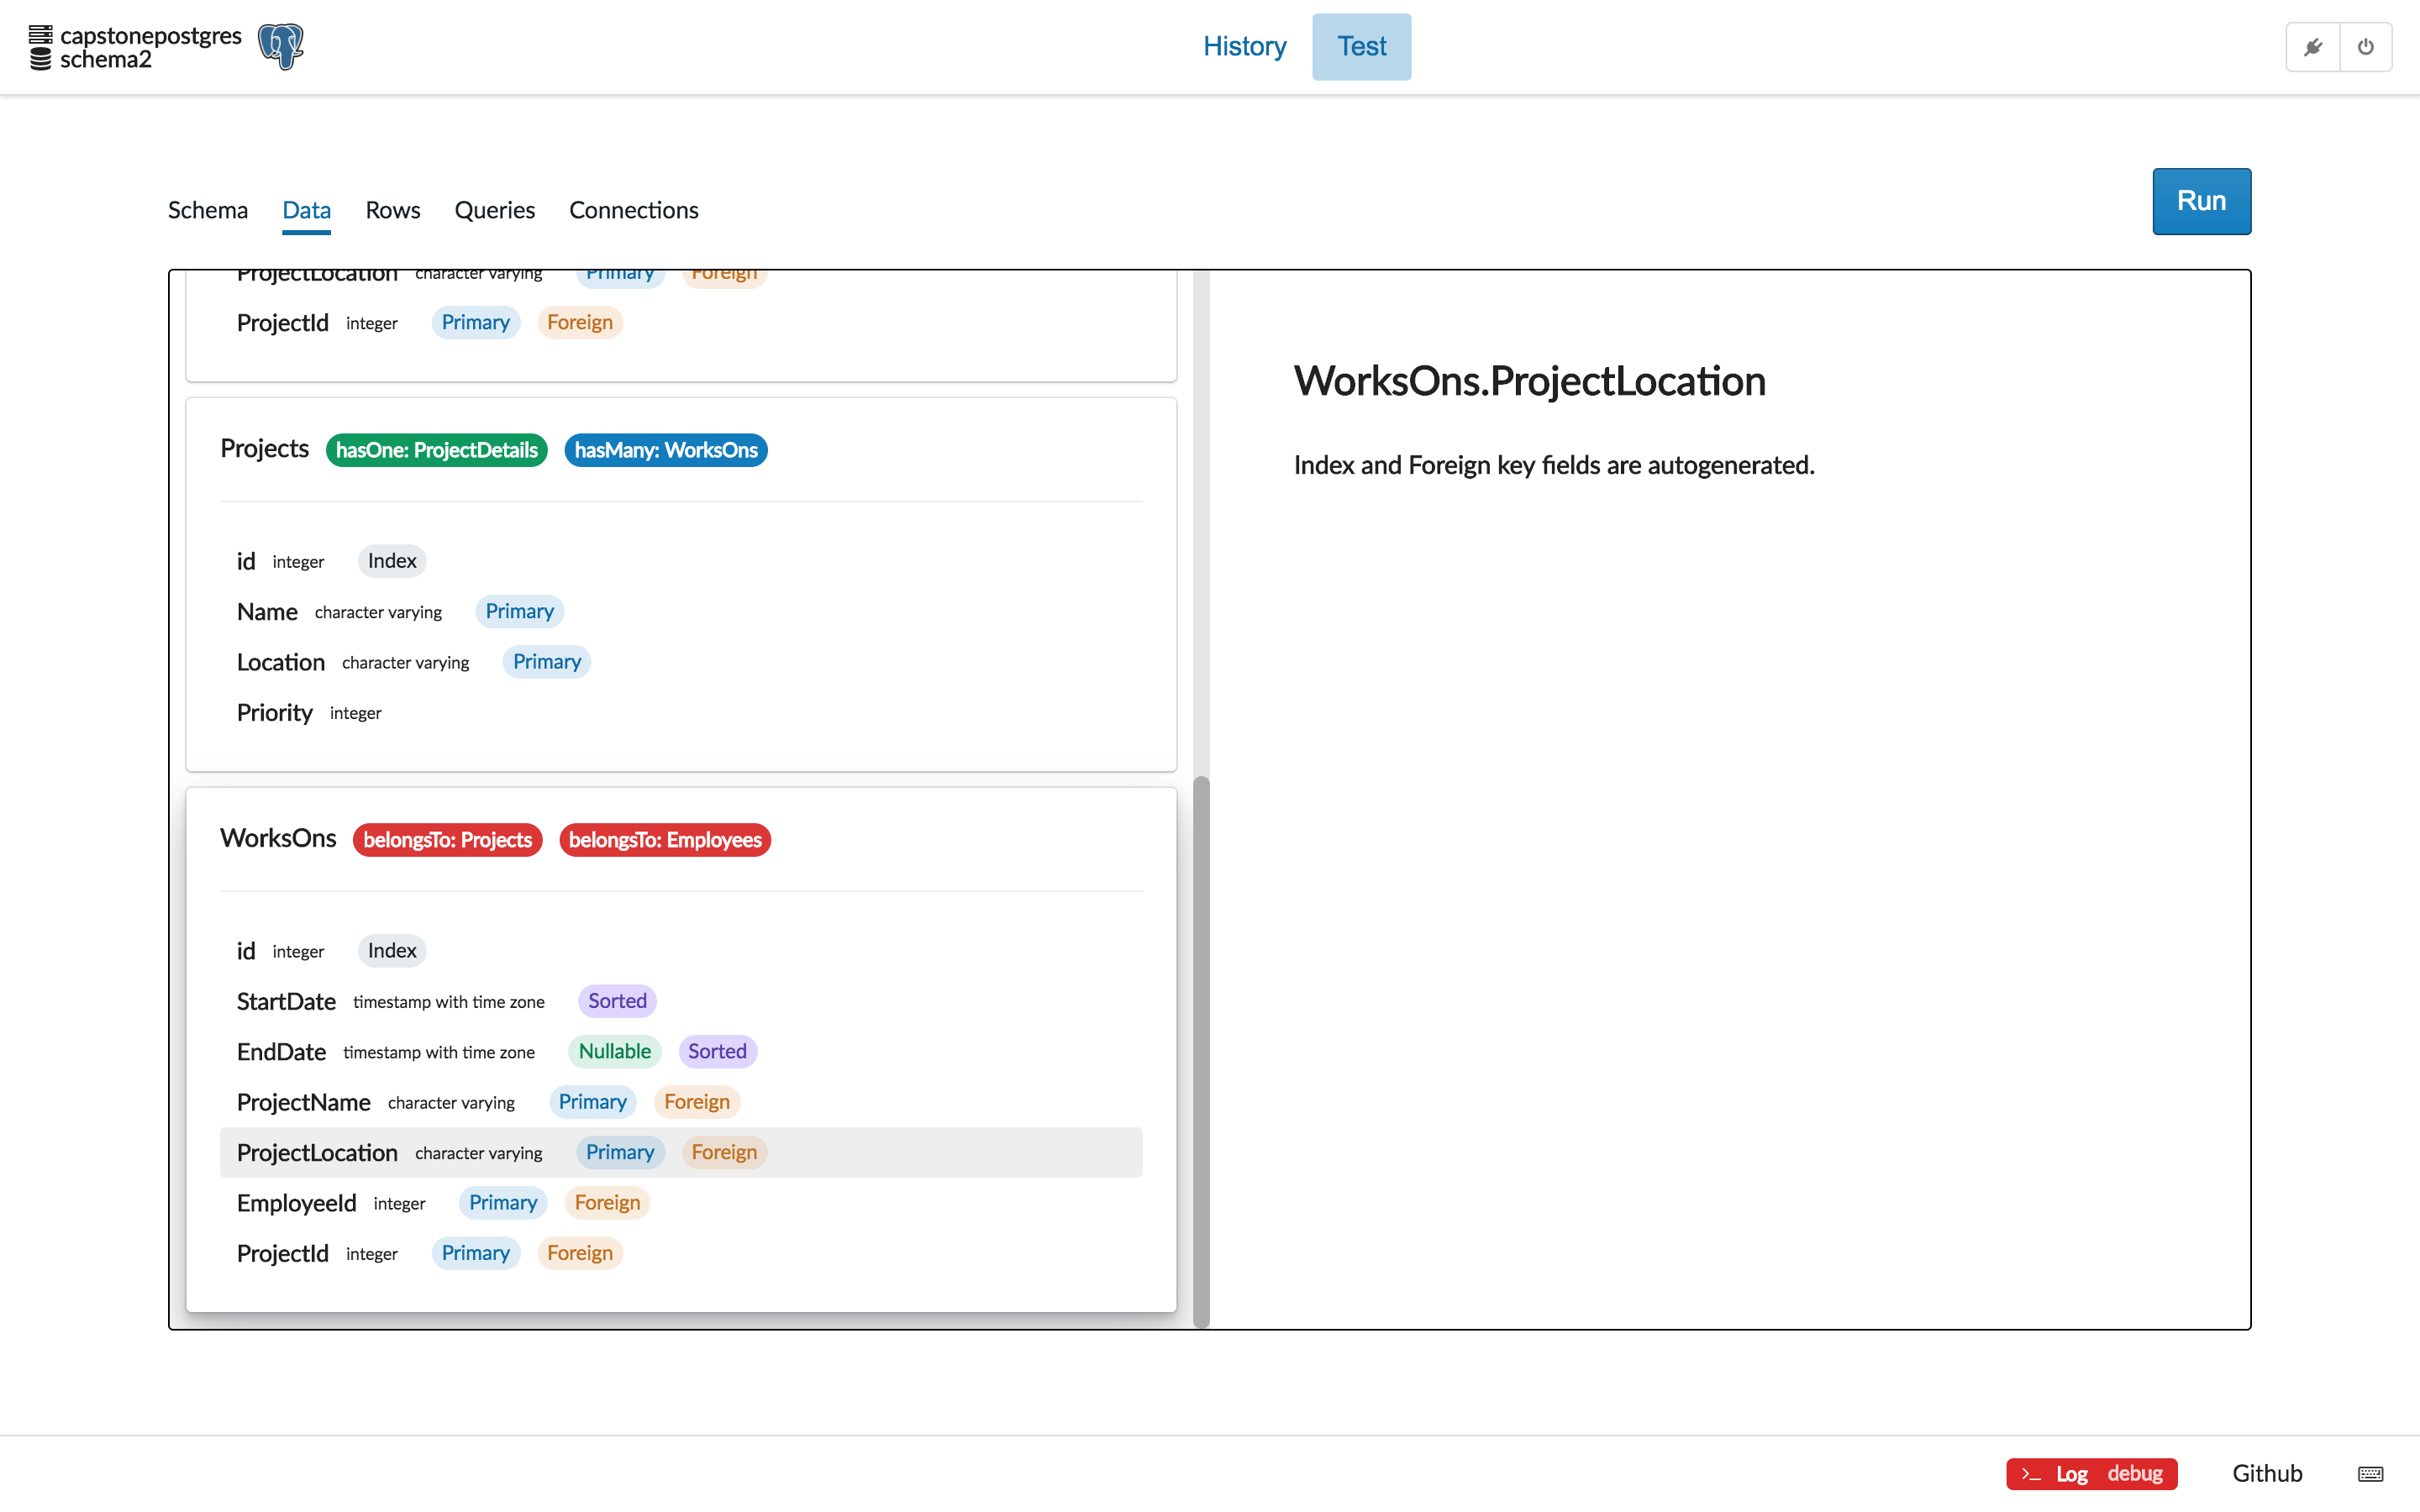
\includegraphics[width=\textwidth]{3-2-2.png}
			\caption{Automatically generated primary and foreign keys }
			
		\end{figure}
		
		In SQLitmus, index and foreign key fields are automatically generated. It is complex to resolve referential constraints, especially for cases where a composite primary key is composed of multiple simple and composite foreign keys (WorkOns table in Figure 9). Thus, such concerns are abstracted away from developers.
		
		
		\begin{figure}[H]
			\centering
			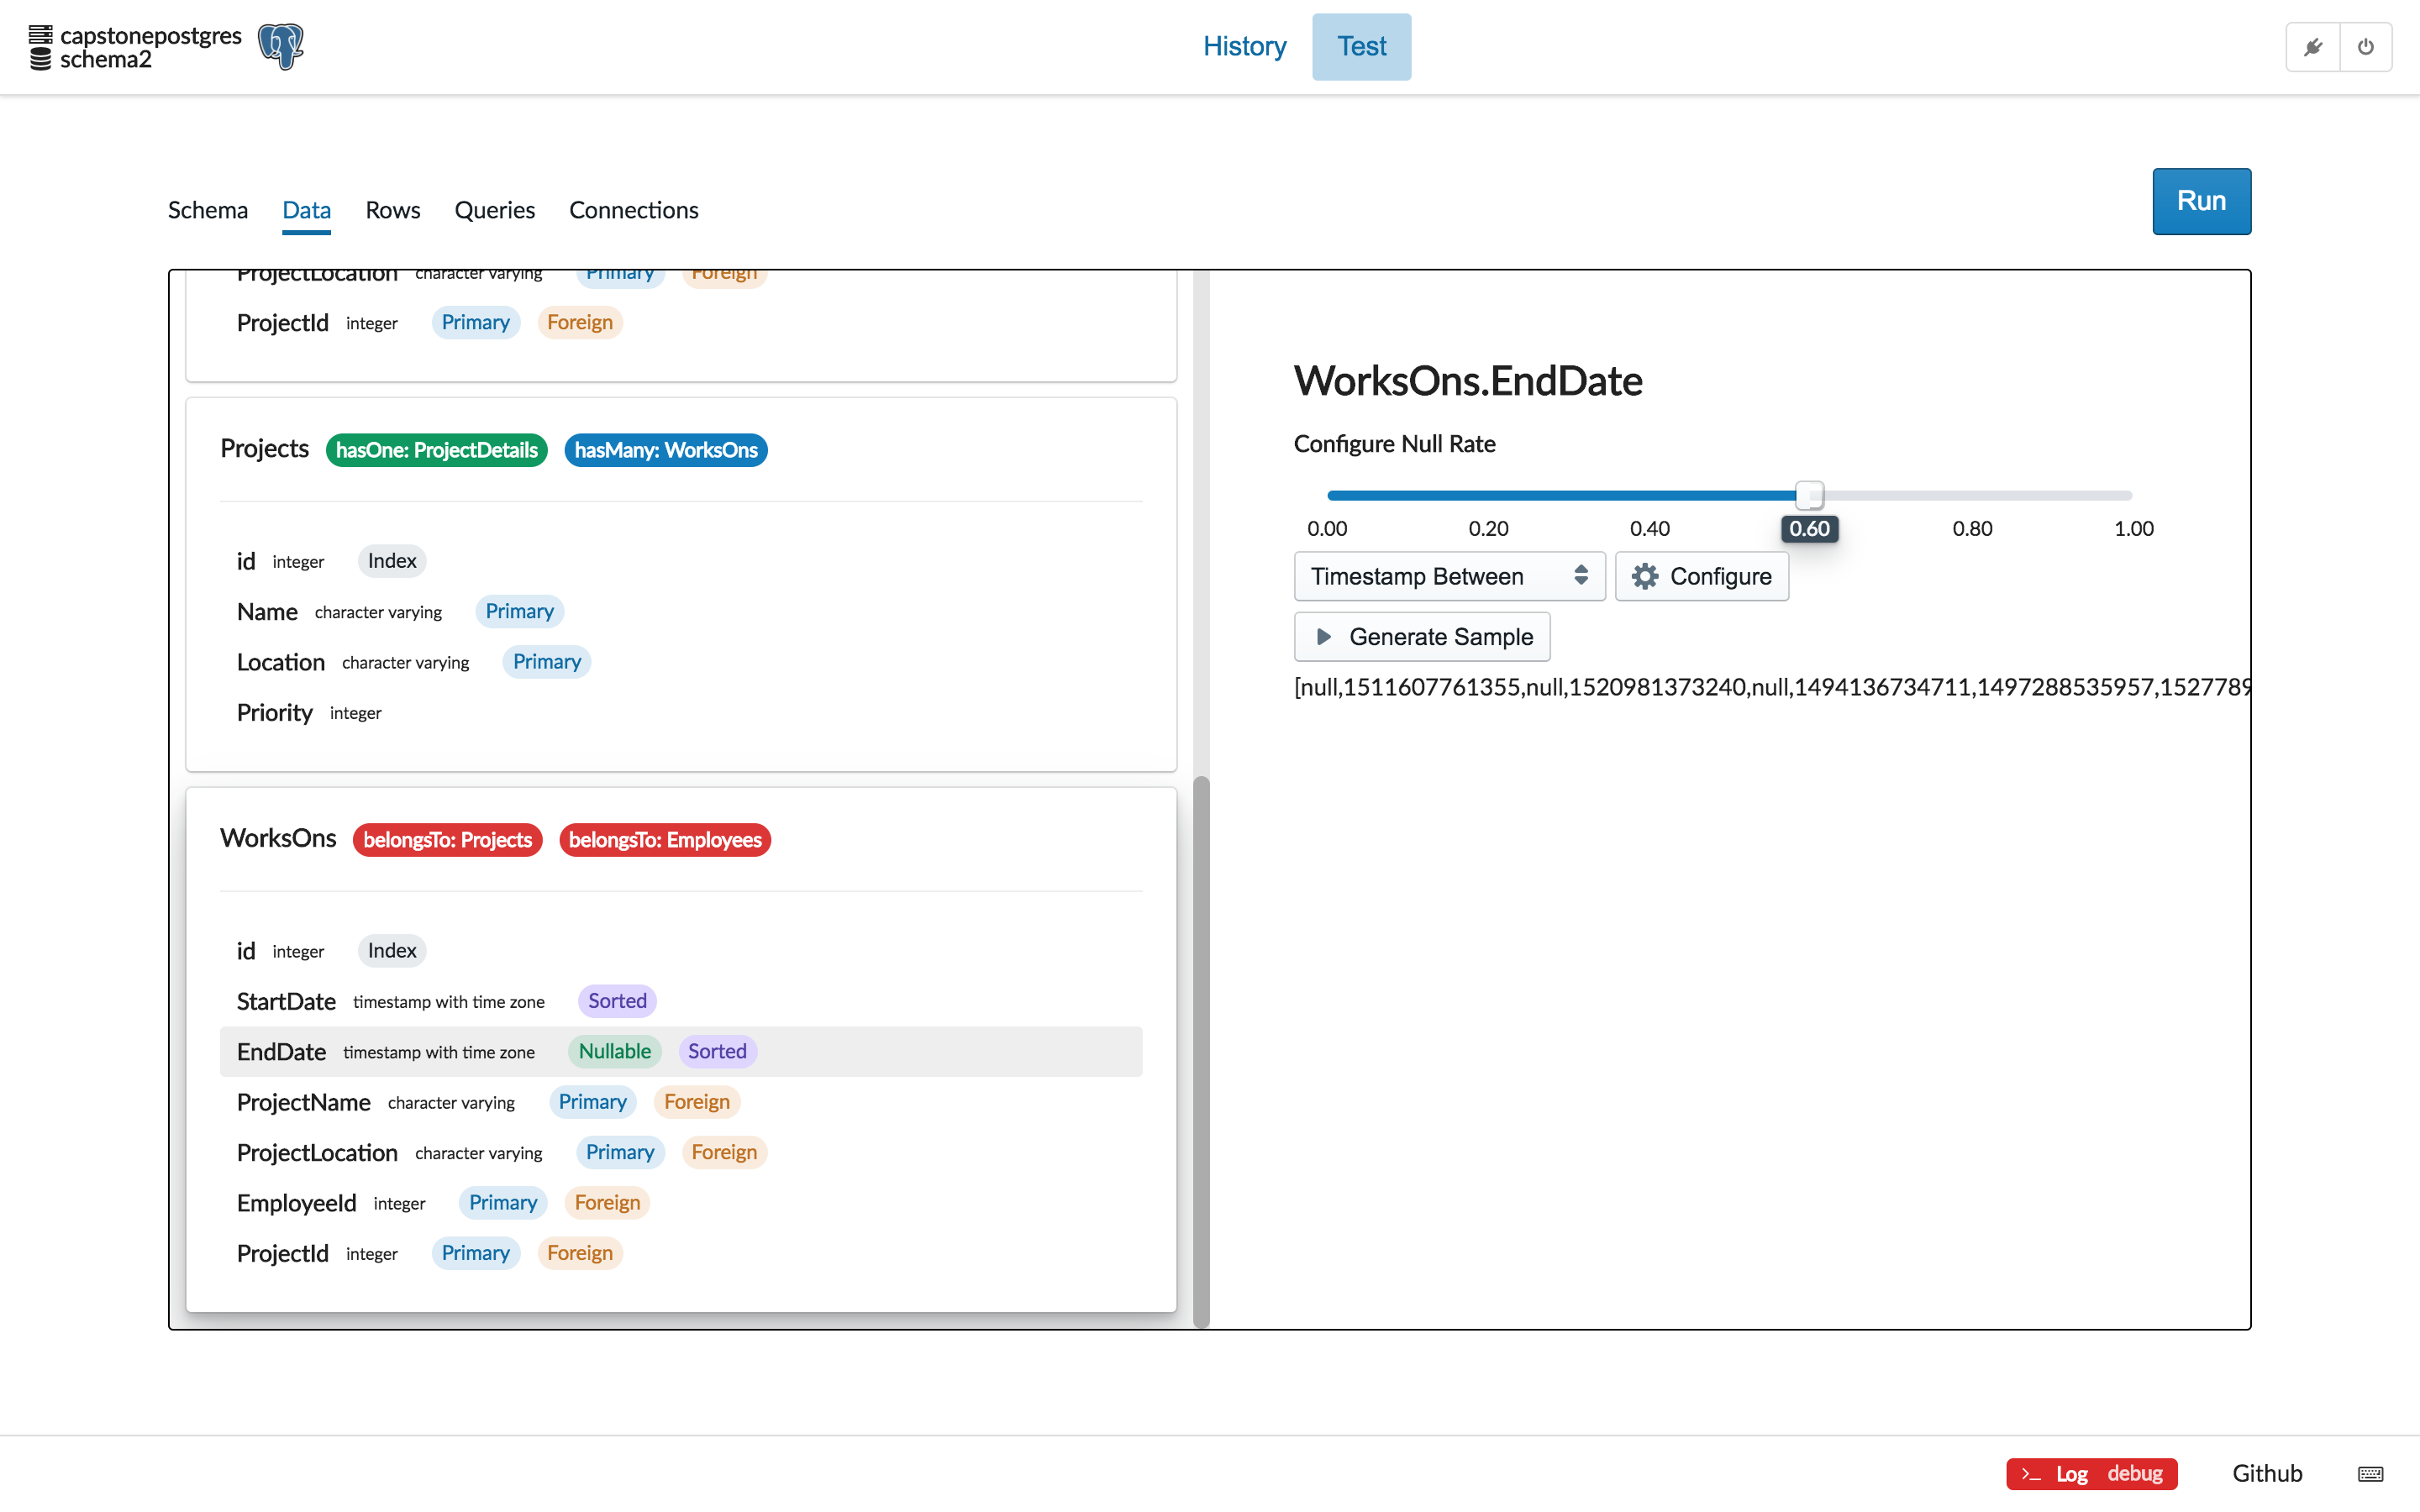
\includegraphics[width=\textwidth]{3-2-2b.png}
			\caption{ Configuring null rates }
			
		\end{figure}
		
		In the case where a nullable field is specified, SQLitmus offers an additional null rate generator that is compatible with all of SQLitmus's 23 built-in and 5 custom data generators. Developers simply has to specify a null rate on top of their chosen data generator. Figure 10 displays the slider in SQLitmus's GUI that configures null rates.
		
		
		\begin{figure}[H]
			\centering
			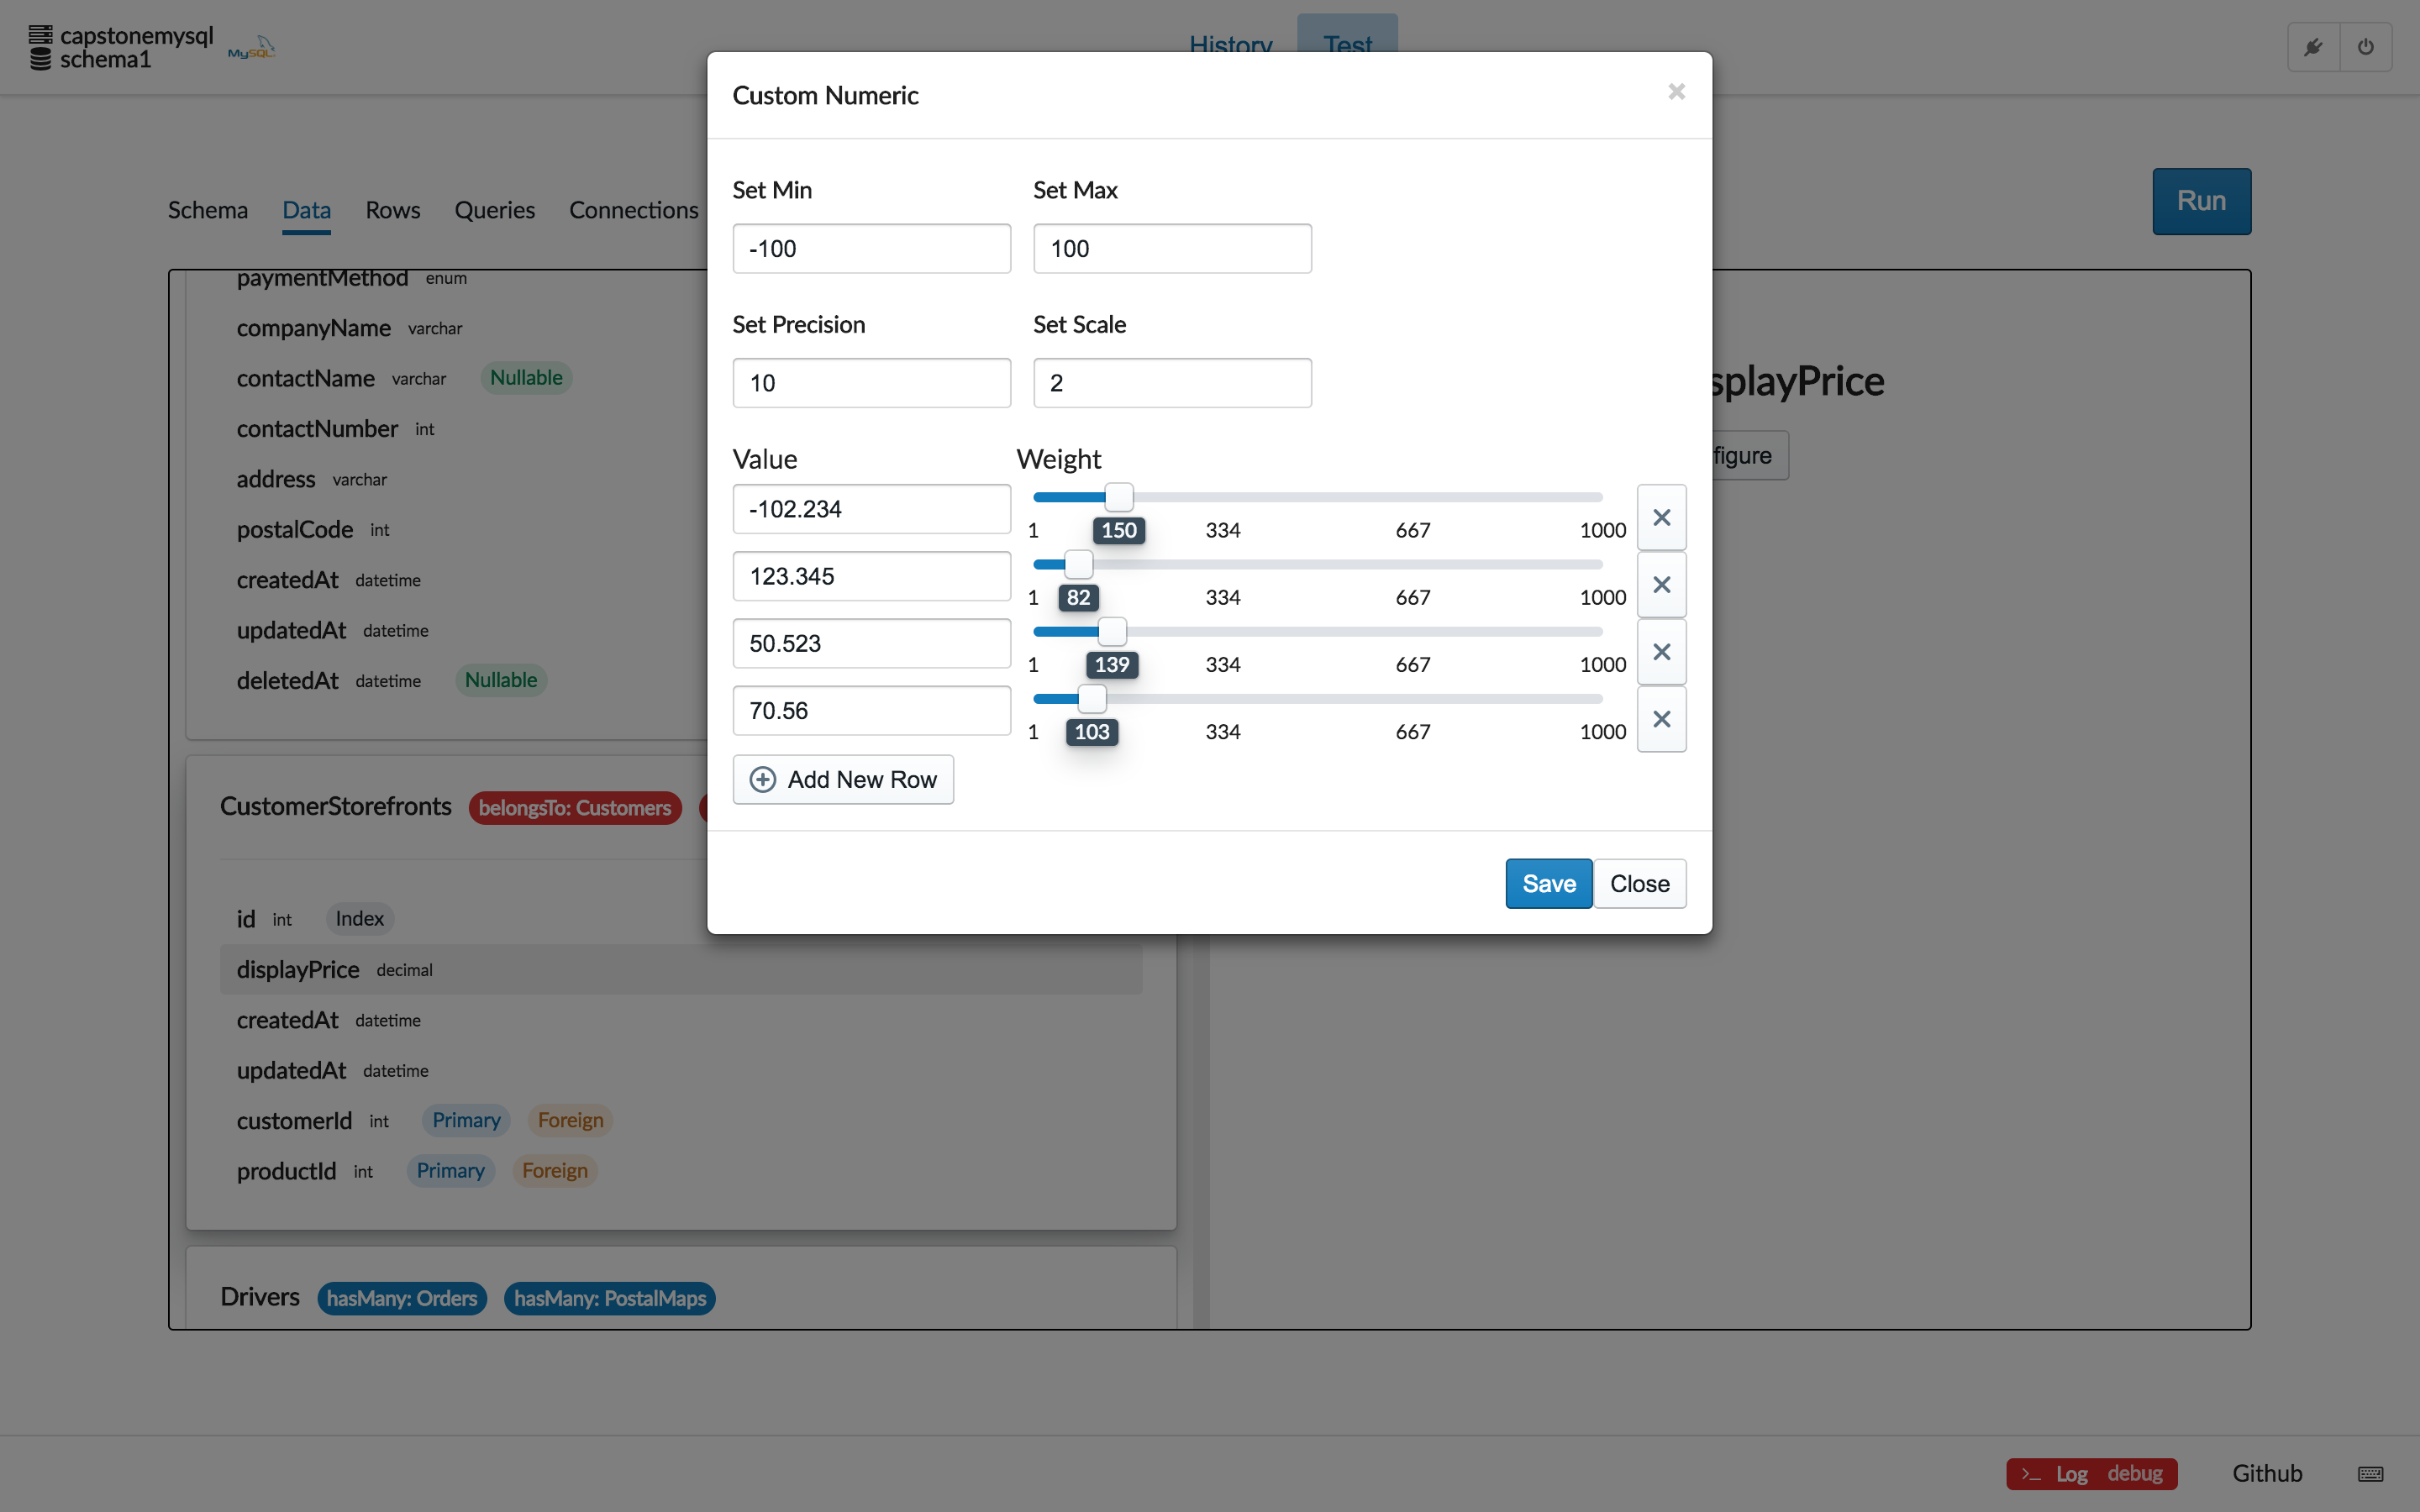
\includegraphics[width=\textwidth]{3-2-2c.png}
			\caption{Data generator configurations }
			
		\end{figure}
		
		Each data generator comes with its own set of configurations which developers are able to access through clicking on the configure button next to the data generator. Some validation rules are common to all generators of a given type (eg. Numerical generators all allow developers to specify min, max, precision\footnote{The number of digits in a number.}, and scale\footnote{The number of digits after the decimal point.} - seen in Figure 11). SQLitmus also ensures that improper validation rules do not affect the integrity of the generated data \footnote{eg. positive scales for integer fields are always considered to be zero}. These validation rules allow developers to generate data that is compatible with the most stringent database settings.
		
		
		\begin{figure}[H]
			\centering
			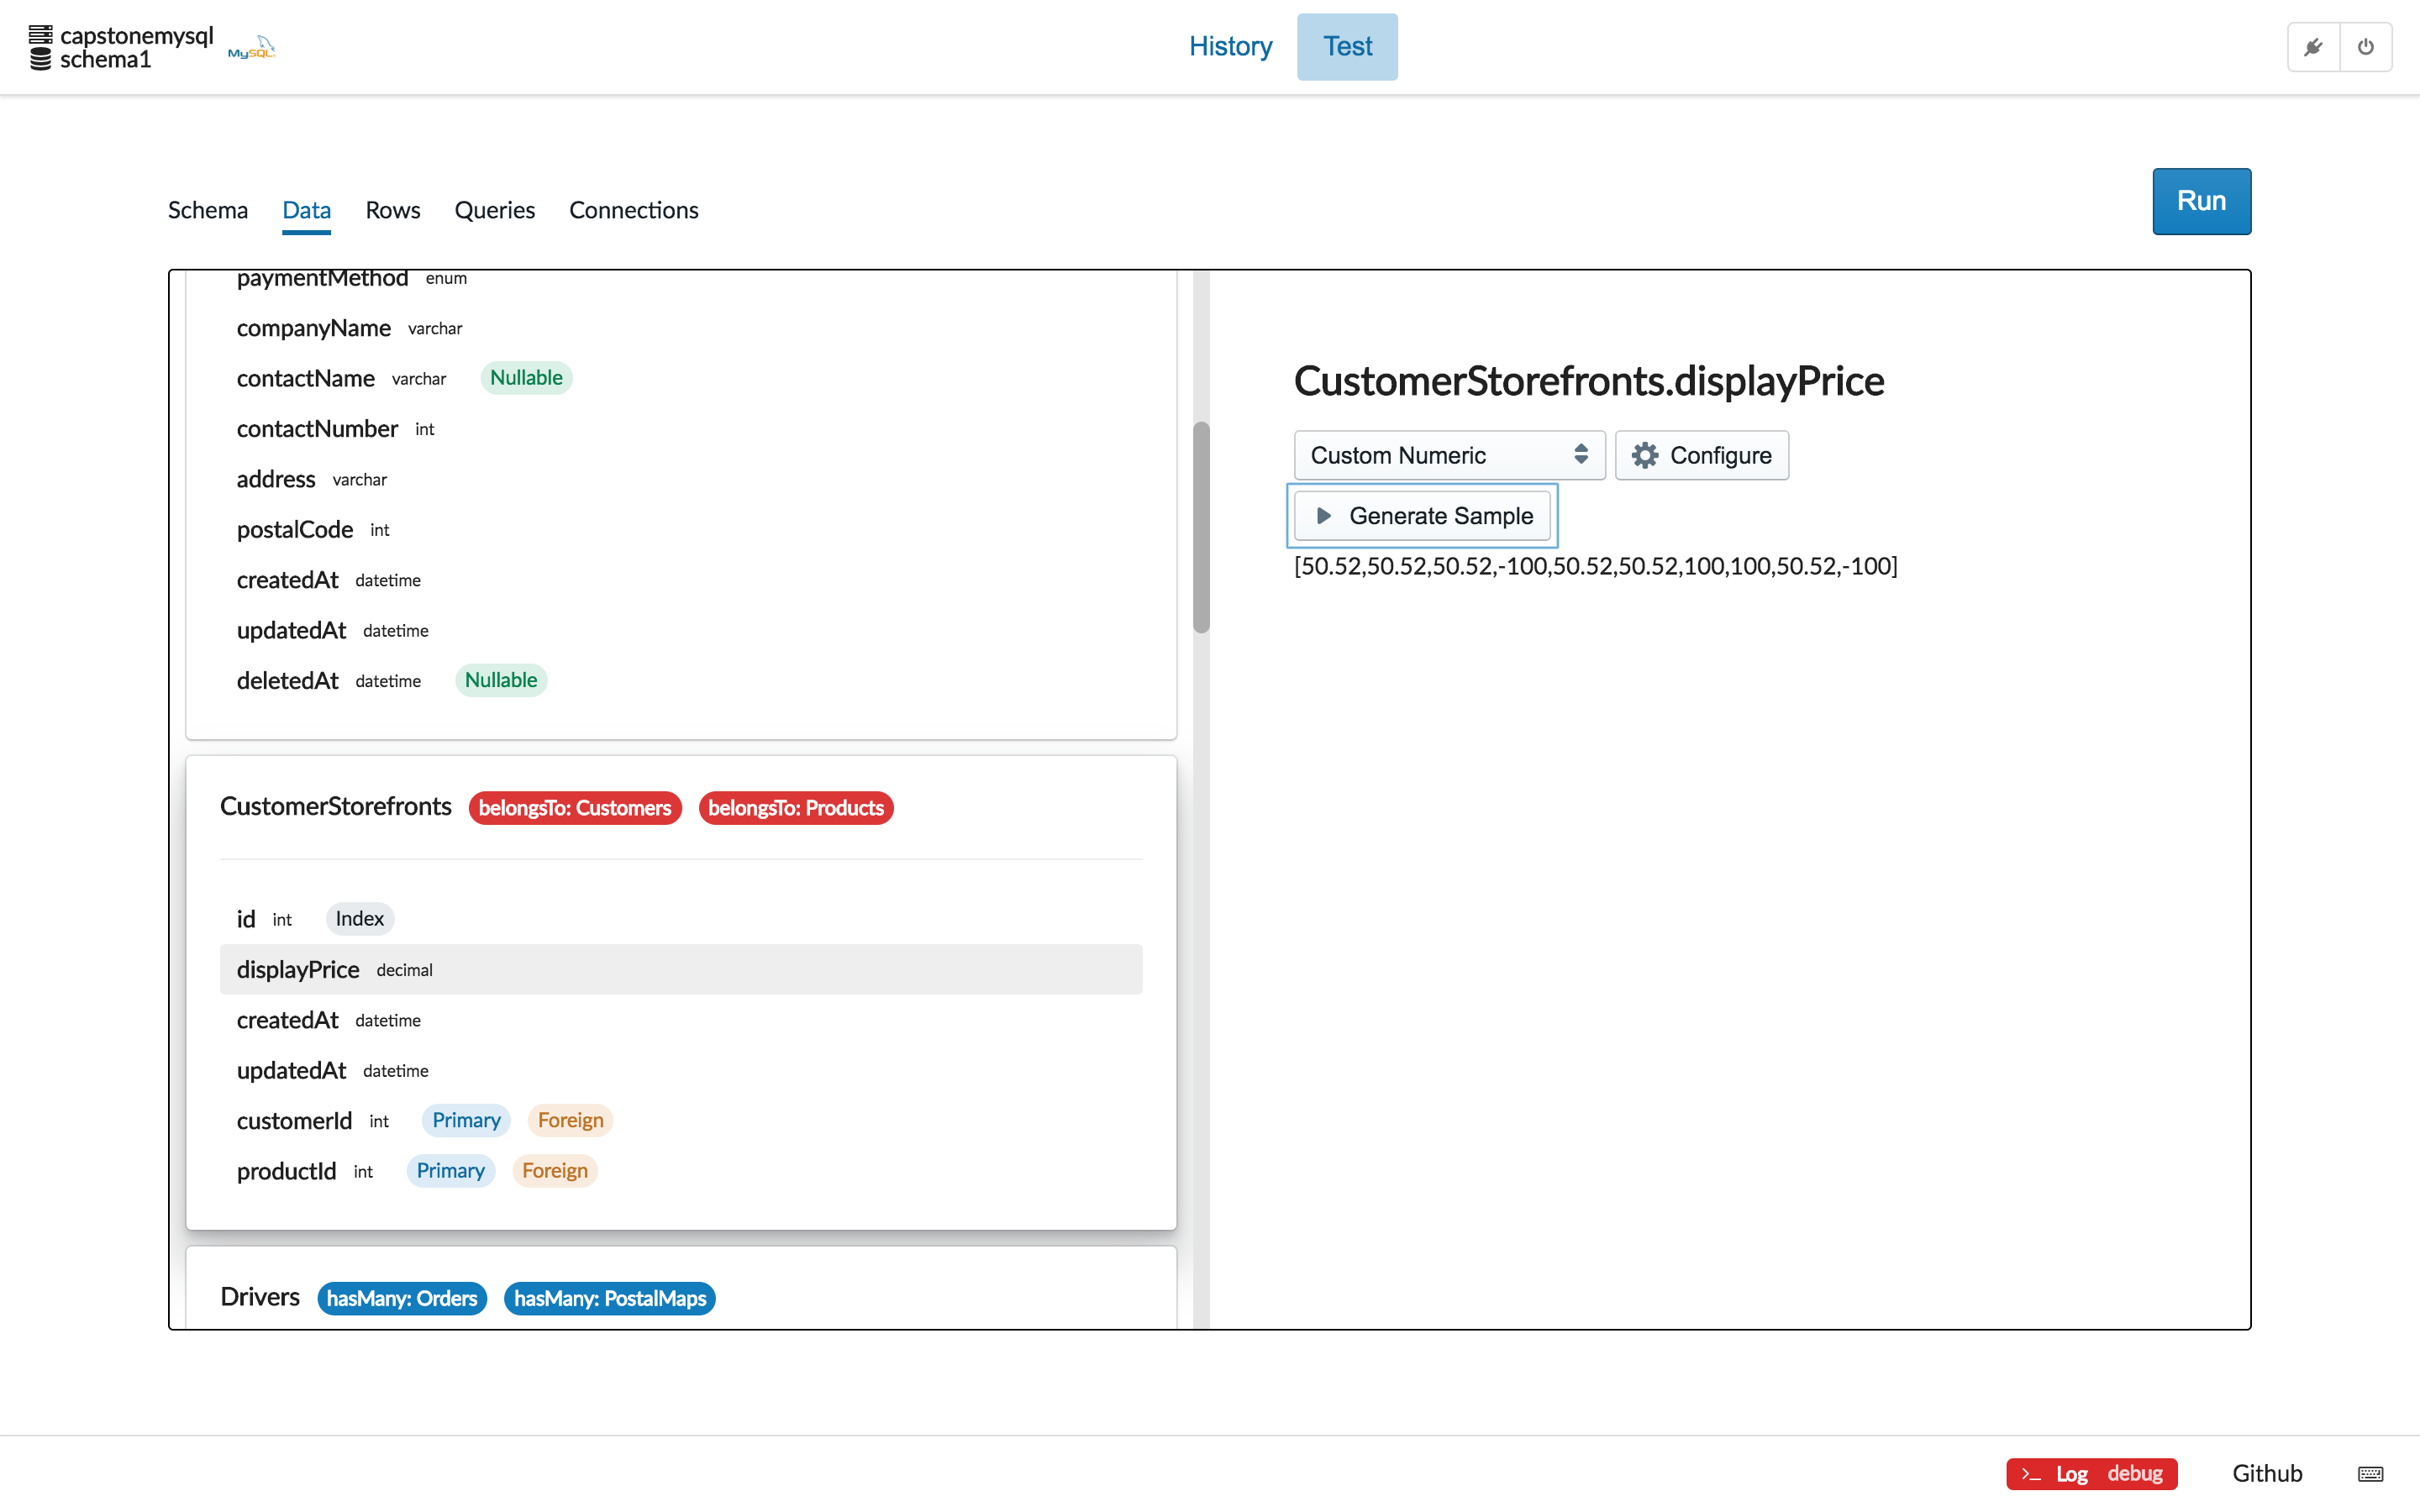
\includegraphics[width=\textwidth]{3-2-2d.png}
			\caption{Sampling data from configured generators }
			
		\end{figure}
		
		Upon successful configuration, developers are able to generate data samples from their customized generator to ensure specification adherence. Figure 12 demonstrates the generation of data samples from a configured generator.
		
		\subsection{Query Generation}
		
		Whereas data generation sets the database up with a valid dataset to prepare it for performance testing, query execution is where performance testing actually occurs. SQLitmus employs the most objective method of performance analysis available: measuring and recording a query's response time.
		
		The query generation feature presented by SQLitmus substantially improves the developer's user experience in configuring test queries. Instead of requiring that developers input an exhaustive list of valid queries, SQLitmus allows developers to specify the types of queries they wish to test their database with. SQLitmus then generates hundreds of randomized valid queries to test the database with for each specified query type. To achieve this end, SQLitmus offers query templating, and a GUI for developers to test the validity of their query templates.
		
		The value of query generation is as follows:
		\begin{itemize}
			\item It is far less rigourous for developers to design a query template as opposed to designing a large set of possible queries to test their database with.
			\item Performance analysis using a static list of queries yields low quality performance data. Databases cache query results, thus identical queries when ran multiple times against the same database, will measure the speed the database takes to deliver a pre-loaded response from its cache rather than the actual time a database takes to process the query.
			\item Since the set of generators used to populate the database is identical to the set of generators used to populate the queries, developers are guaranteed to generate valid queries and benefit from the high likelihood of their queries targetting actual data in the database.
		\end{itemize}
		
		\subsubsection{Query Templating}
		
		Developers are often more interested in finding out the performance of a type of query as compared to the performance of an actual specific query. Developers also do not wish to relearn a new Domain Specific Language to specify their types of queries, and wish to test the exact queries executed in production.
		
		Query templates afford developers the ability to generate multiple queries from a single template . 
		
		
		
		\begin{minted}[bgcolor=light-gray,fontsize=\footnotesize,baselinestretch=1.2,linenos]{sql}
		-- WorksFor targets the index of another row in the Employees table and
		-- specifies a supervisor-subordinate relationship
		SELECT * FROM Employees WHERE WorksFor=${Employees.RANDROW};
		\end{minted}
		
		
		For instance, the above code snippet demonstrates how a simple query template in SQLitmus allows developers to test for their database's ability to retrieve all subordinates of a randomized Employee. Compare this to having the developers specify a static list of queries.
		
		\begin{minted}[bgcolor=light-gray,fontsize=\footnotesize,baselinestretch=1.2,linenos]{mysql}
		SELECT * FROM Employees WHERE WorksFor=1;
		SELECT * FROM Employees WHERE WorksFor=2304;
		SELECT * FROM Employees WHERE WorksFor=3520392;
		\end{minted}
		
		
		Not only is templating much more convenient, it also has a low learning curve. The template above also guarantees that the substituted value belongs to the same domain as the data generated in the WorksFor column.
		
		Expressions nested between a dollar sign and curly braces \mintinline{javascript}{${expression}} are parsed by the query preprocessor and replaced by an appropriate value.
		
		In the above case, SQLitmus will replace the expression with a randomly generated row index from the Employees table. 
		
		Beyond generating substitution rules, SQLitmus's query templates affords developers with the ability to setup their queries (to ensure that an actual workload is being measured) and perform clean-ups (to ensure that INSERT or DELETE queries do not cause a substantial cardinality drift) through the use of special delimiters.
		
		\begin{minted}[bgcolor=light-gray,fontsize=\footnotesize,baselinestretch=1.2,linenos]{mysql}
		-- Insert new employee (MySQL)
		-- Values are (id, EmploymentDate, FirstName, LastName, SSN, WorksFor)
		-- SSN is the primary key
		-- Only queries specified between the begin and end delimiters will
		-- have their response time measured.
		DELETE FROM Employees WHERE SSN = ${Employees.SSN};
		
		${BEGIN.DELIMITER}
		
		INSERT INTO Employees VALUES 
		(null,FROM_UNIXTIME(CEIL(${Employees.EmploymentDate}/1000)),
		${Employees.FirstName},${Employees.LastName}, 
		${Employees.SSN}, ${Employees.RANDROW});
		
		${END.DELIMITER}
		
		DELETE FROM Employees WHERE SSN = ${Employees.SSN};
	\end{minted}
	
	
	For instance, if a developer is interested in testing the time taken to INSERT a new employee record into his/her database, the query response time measurement should ideally reflect the time it takes to INSERT an actual row of employee data into the database. 
	
	SQLitmus's query template allows developers to first DELETE any conflicting employee record/records from the database before testing the time it takes for the database to INSERT an actual row of employee data. This functionality allows SQLitmus to yield a more accurate query response time measurement as compared to QGEN. 
	
	The impact of the INSERT workload on the cardinality drift of the Employees table can also be mitigated through specifying an additional DELETE statement after the INSERT is performed. Cardinality drifts are thus much more well accounted for in SQLitmus as compared to QGEN.
	
	
	\begin{figure}[H]
		\centering
		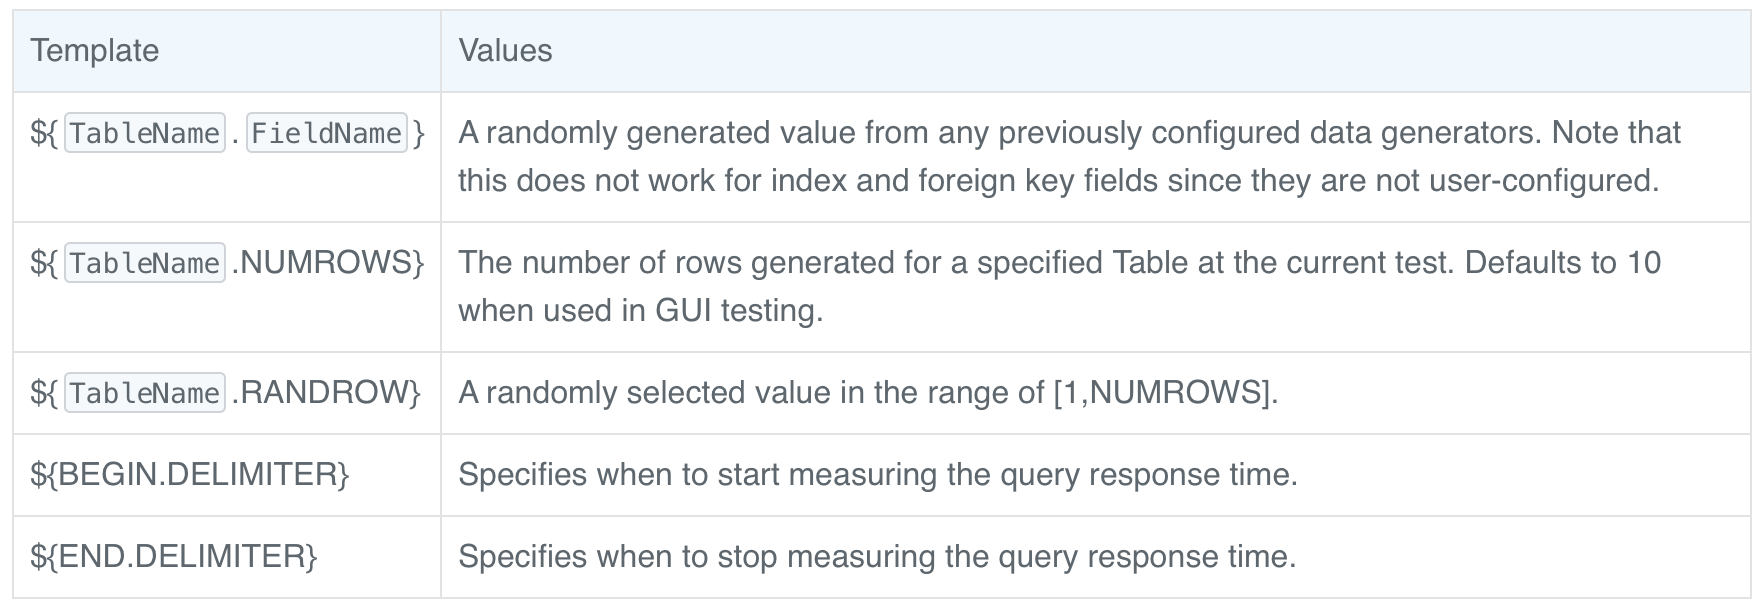
\includegraphics[width=\textwidth]{3-3-1.png}
		\caption{Full set of Query templating options available in SQLitmus }
		
	\end{figure}
	
	Figure 13 displays the full set of Query Templating options available in SQLitmus. This combination of templating options allows developers to populate their query templates with random values that belong to the same domain as any given field of interest.
	
	For index fields, developers can use the \mintinline{javascript}{${TableName.RANDROW}} templating option to generate a random index of the same domain as the generated data-set.
	
	For non-index and foreign key fields, the \mintinline{javascript}{${TableName.FieldName}} option is available.
	
	All foreign key fields necessarily references a root non-foreign key target. For instance, if Table1.Field1 references Table2.Field2, developers can simply use the \mintinline{javascript}{${Table2.Field2}} generator to generate values for Table1.Field1. \footnote{ Use \mintinline{javascript}{${Table2.RANDROW}} instead if Field2 is an index key}
	
	The following scenario demonstrates how the various query templating options can be used together to insert a new row of employee data of the same domain as the generated data-set.
	
	
	\begin{minted}[bgcolor=light-gray,fontsize=\footnotesize,baselinestretch=1.2,linenos]{mysql}
	-- Staffing an employee on a project (PostgreSQL)
	-- (id, StartDate, EndDate, ProjectName, ProjectLocation, EmployeeId, ProjectId)
	-- ProjectName, ProjectLocation, and ProjectId addresses the 
	-- Name, Location, and id fields of the Projects table respectively.
	-- EmployeeId addresses the id field of the Employees table.
	INSERT INTO "WorksOns" VALUES (DEFAULT, 
	to_timestamp(CEIL(${WorksOns.StartDate}/1000)), 
	to_timestamp(CEIL(${WorksOns.EndDate}/1000)),
	${Projects.Name},${Projects.Location},
	${Employees.RANDROW},${Projects.RANDROW});
	\end{minted}
	
	\begin{itemize}
		\item StartDate and EndDate has directly accessible generators \mintinline{javascript}{${WorksOns.StartDate}} and \mintinline{javascript}{${WorksOns.EndDate}} so we supply them accordingly.
		\item ProjectName and ProjectLocation references non-index fields Projects.Name and Projects.Location so we supply \mintinline{javascript}{${Projects.Name}} and \mintinline{javascript}{${Projects.Location}} accordingly.
		\item EmployeeId and ProjectId references the indexes of the Employees and Projects tables so we supply \mintinline{javascript}{${Employees.RANDROW}} and \mintinline{javascript}{${Projects.RANDROW}} accordingly.
	\end{itemize}
	
	
	All queries generated are deteministically random, so developers are able to execute the same set of randomly generated queries across different databases and different trials of the same test.
	
	
	
	\subsection{ Query Template GUI}
	
	Regardless of how simple it is to use the query templating system, developers need a way of testing the validity of their query templates ahead of running any performance analyses. Developers also need a way to persist the list of already configured query templates in the software so that they do not have to spend time re-configuring the list of queries templates that they have used in a previous test.
	
	Similar to the database connection management module, the query template GUI has also been forked from SQLectron. The SQLectron query browser natively supports tabs, query execution, and query auto-completion.
	
	\begin{figure}[H]
		\centering
		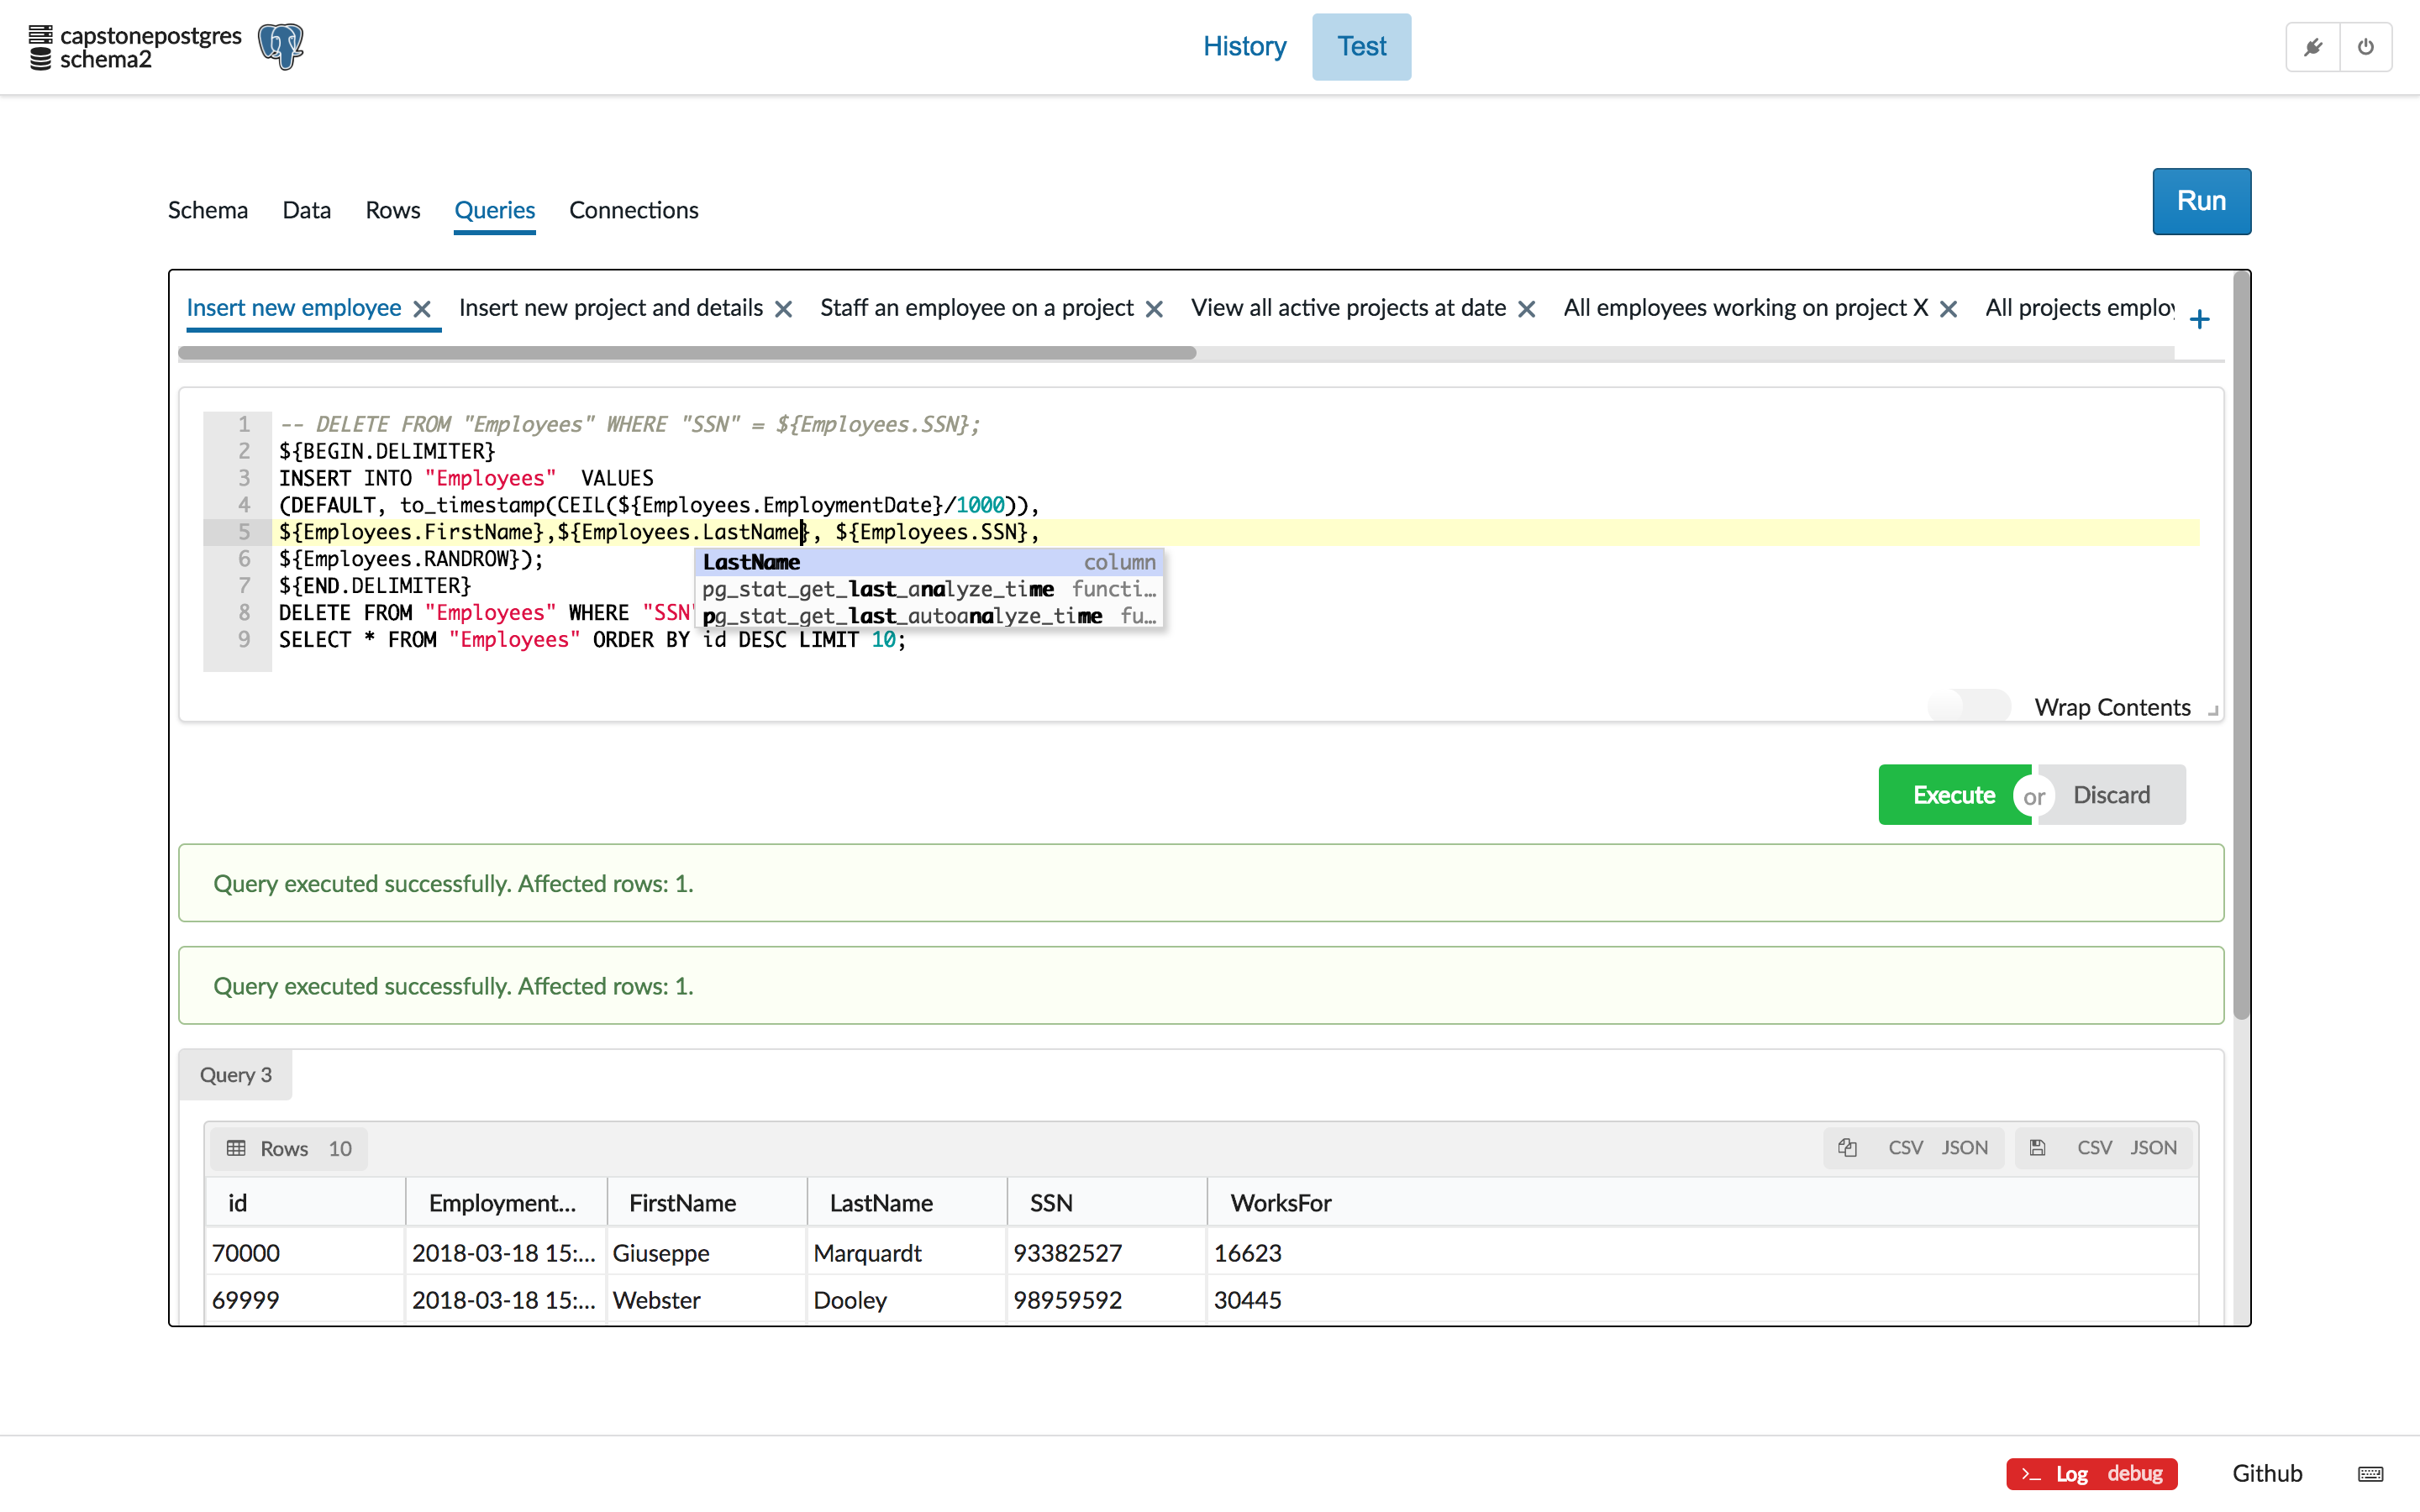
\includegraphics[width=\textwidth]{3-3-2.png}
		\caption{Query Template GUI }
		
	\end{figure}
	
	SQLitmus extends the query browser of SQLectron by offering tab persistence, query template preprocessing, autocompletion of SQLitmus templating options, and a modified GUI that fits SQLitmus's overall design better. While the GUI (as shown in Figure 14) is densely packed, it still offers a good user experience for developers working on the SQLitmus platform.
	
	Developers are able to test all available SQLitmus templating options within the GUI itself. Without any additional configurations, the query template preprocessor populates the query templates with values generated from the already configured data generators. All test queries executed also target the same database that the developer is currently connected to.
	
	
	\subsection{Test Configurations}
	
	Developers do not simply wish to test the performance of their SQL database in a single environment. They wish to test their database under multiple environments so that they are able to identify trends that are important to them such as:
	\begin{itemize}
		\item How well their SQL database's performance scales with the amount of data it holds.
		\item How well their SQL database's performance scales with the number of concurrent requests it serves.
	\end{itemize}
	
	
	The following test configurations allow developers to specify up to 25 different environments to test their SQL database under in a single run.
	
	\subsubsection{Row Configurations}
	
	\begin{figure}[H]
		\centering
		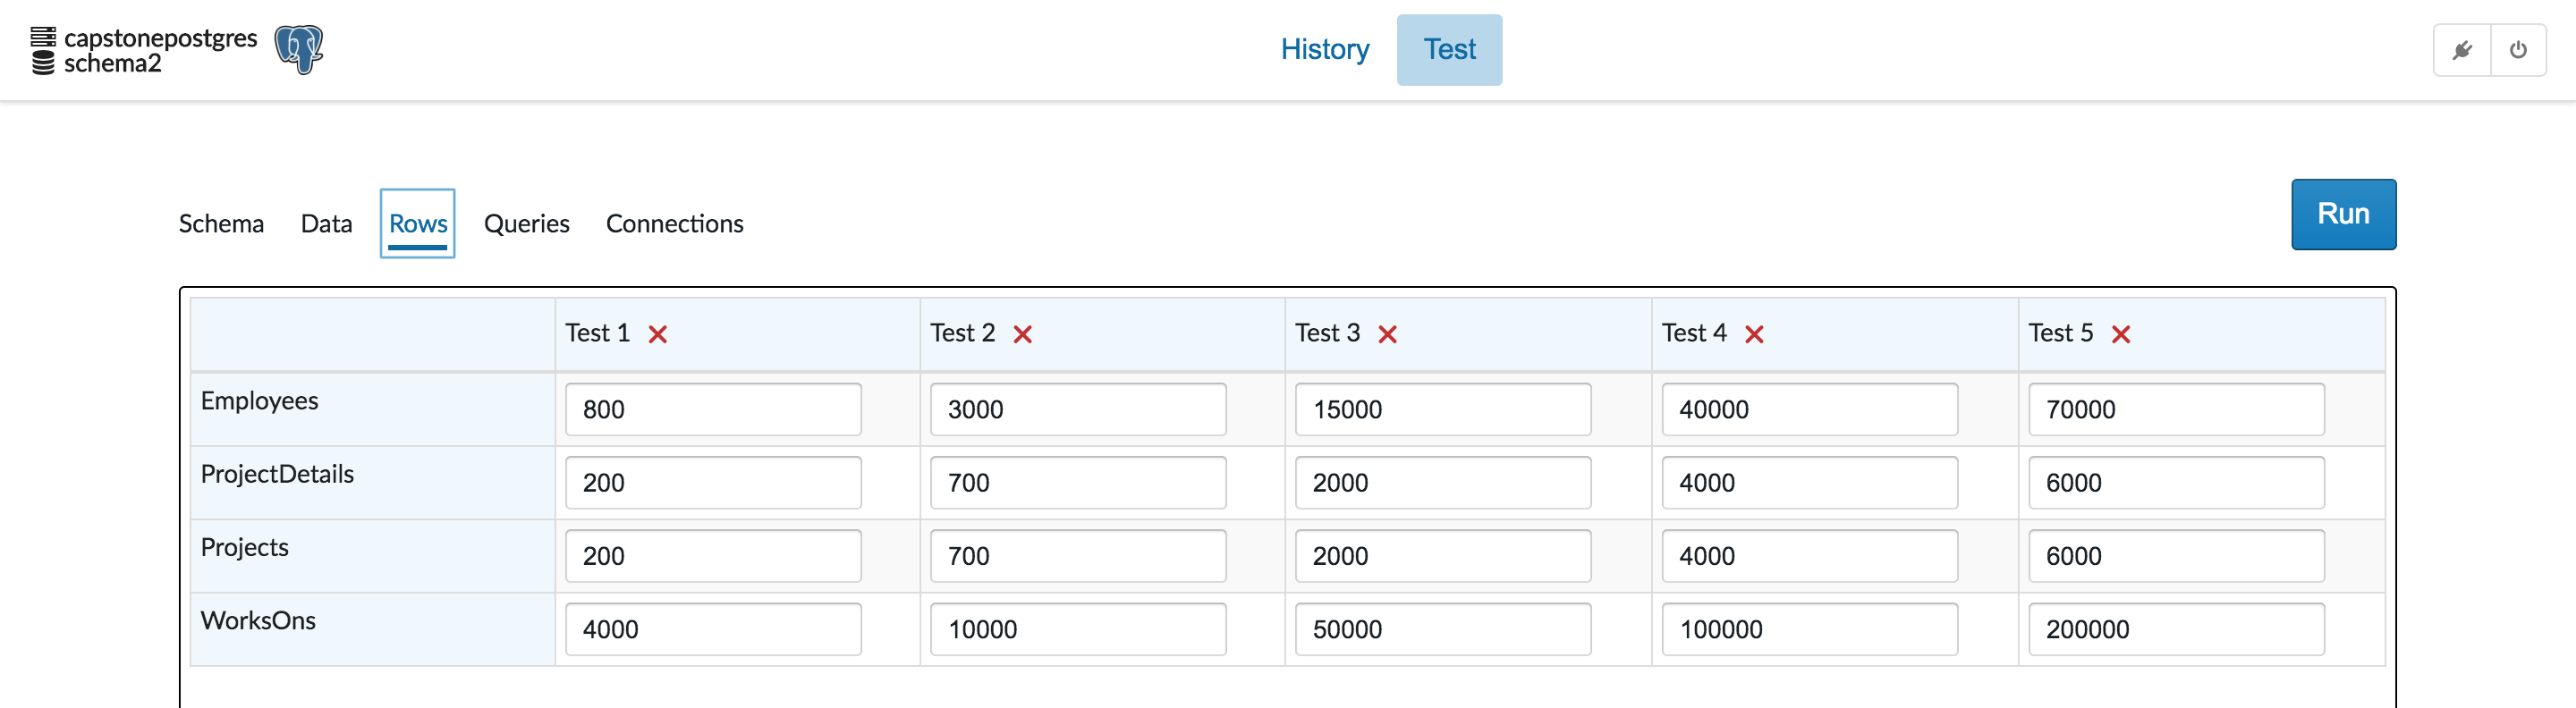
\includegraphics[width=\textwidth]{3-4-1.png}
		\caption{Row Configuration GUI }
		
	\end{figure}
	
	The row configurations tab (as shown in Figure 15) allows developers to specify the number of rows of data they wish to generate on a tabular level. Developers are allowed to specify up to five test trials in a single run of performance analysis.
	
	As the data generated in the last specified test persists in the database, developers who are not concerned with SQL performance testing can still use SQLitmus as a pure test data generation tool. This allows them to re-purpose SQLitmus for API performance testing, and user interface development testing.
	
	\begin{figure}[H]
		\centering
		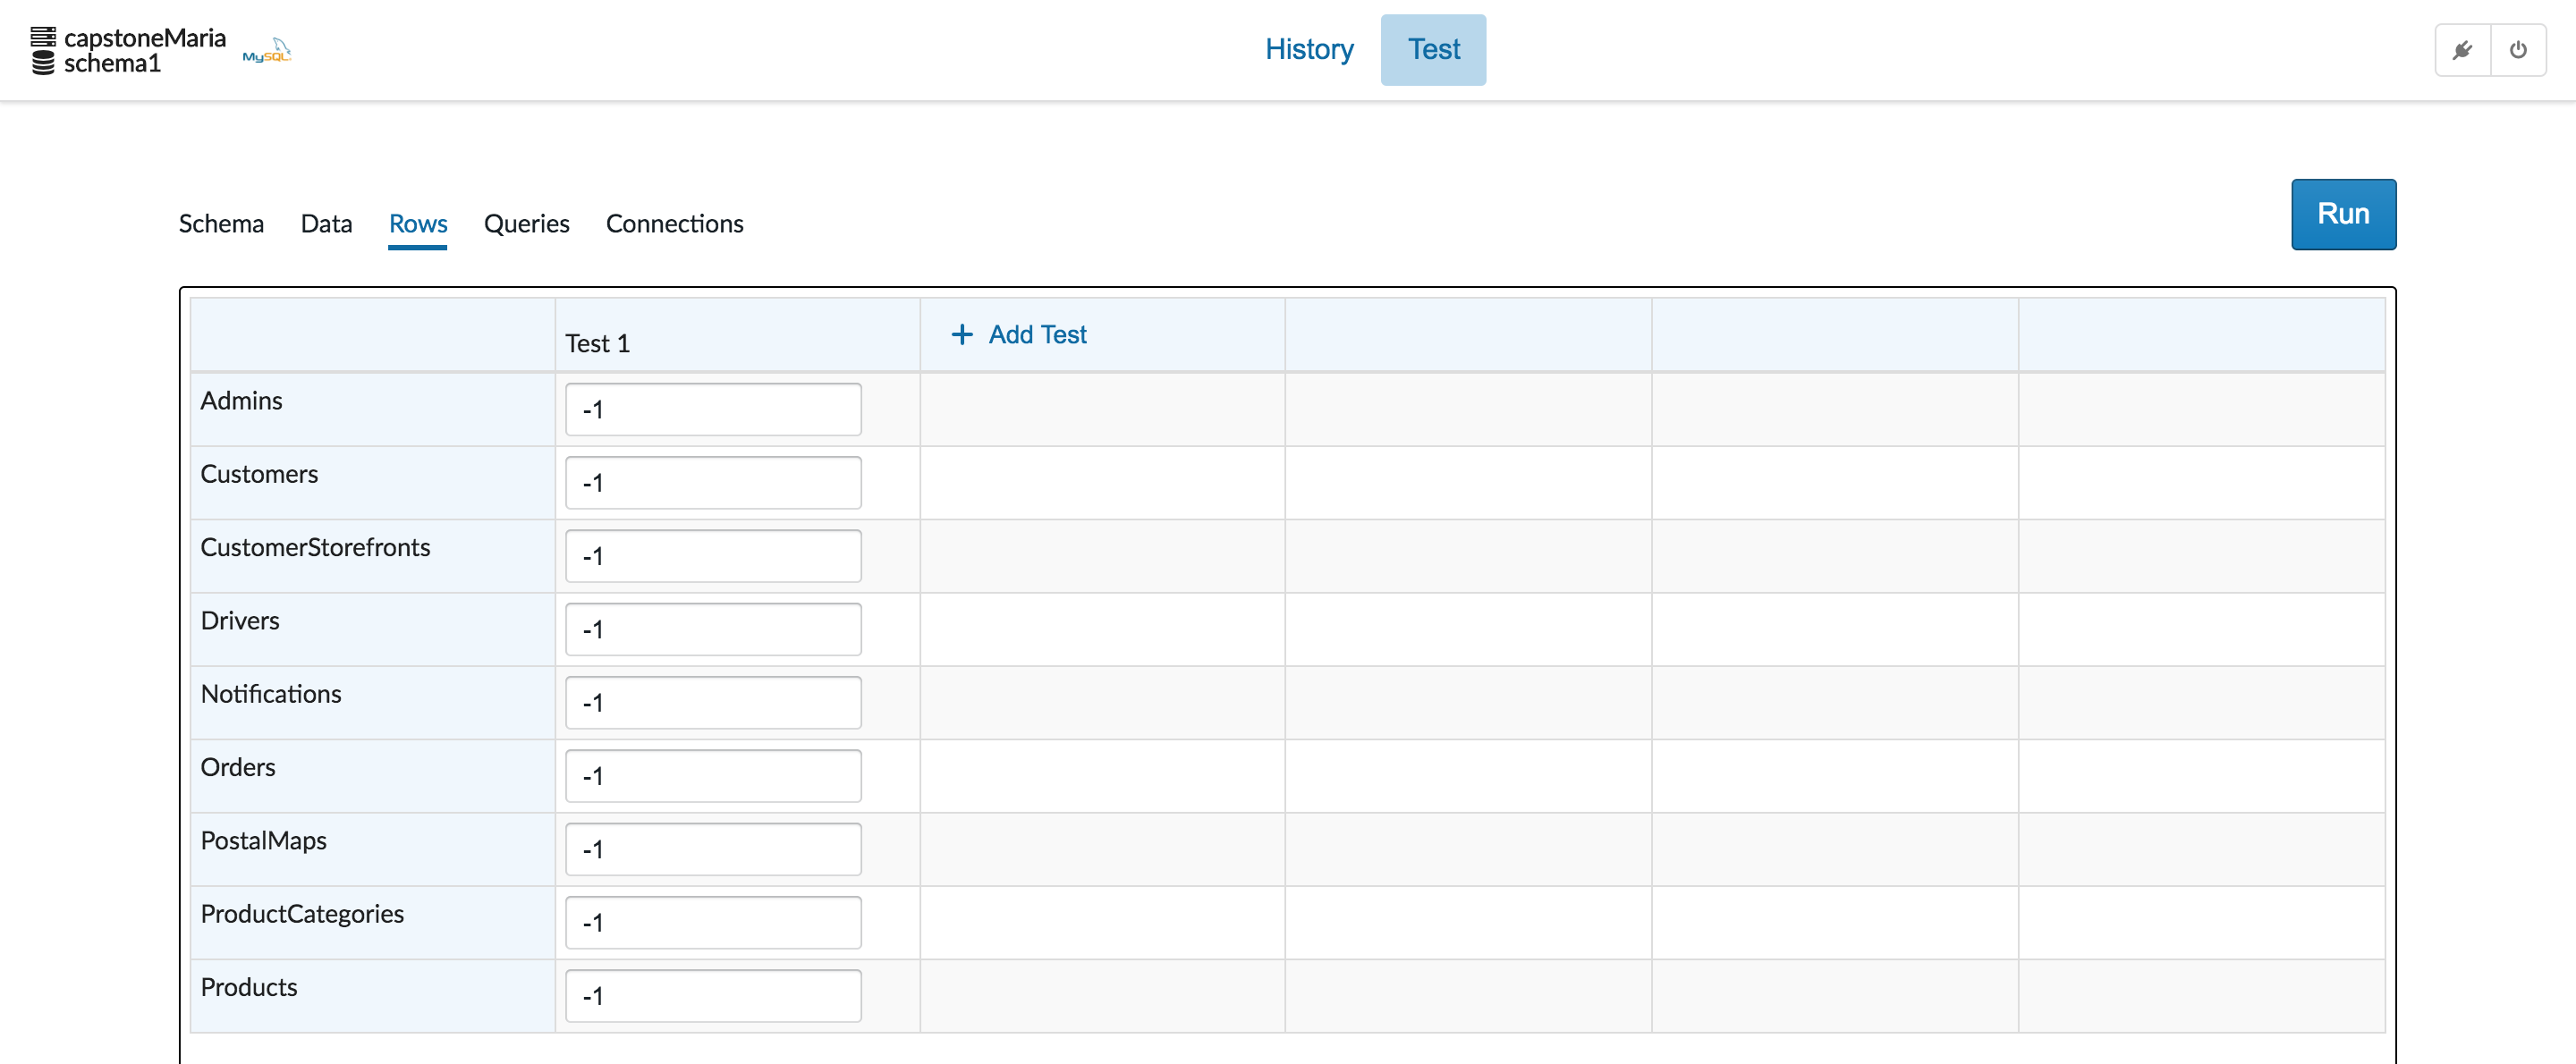
\includegraphics[width=\textwidth]{3-4-1b.png}
		\caption{Bypassing data generation through invalid row configurations }
		
	\end{figure}
	
	The author of SQLitmus also recognizes that SQLitmus is neither the fastest, most robust, nor most expressive test data generator available in the market. As such, SQLitmus provides a way for developers using other test data generation tools to bypass SQLitmus's data generation process to solely capitalize on SQLitmus's query templating and performance testing engine to measure their database's performance. Figure 16 shows an example of bypassing data generation in SQLitmus.
	
	If at least one input is configured with an invalid number of rows - being any negative integer - SQLitmus will skip the data generation process and proceed directly to executing the performance test. 
	
	If all rows are supplied with zero, SQLitmus wipes the database clean of any test data and resets all automatically incrementing counters present on the database to their default values.
	
	\subsubsection{ Max Connection Pool Configurations}
	
	\begin{figure}[H]
		\centering
		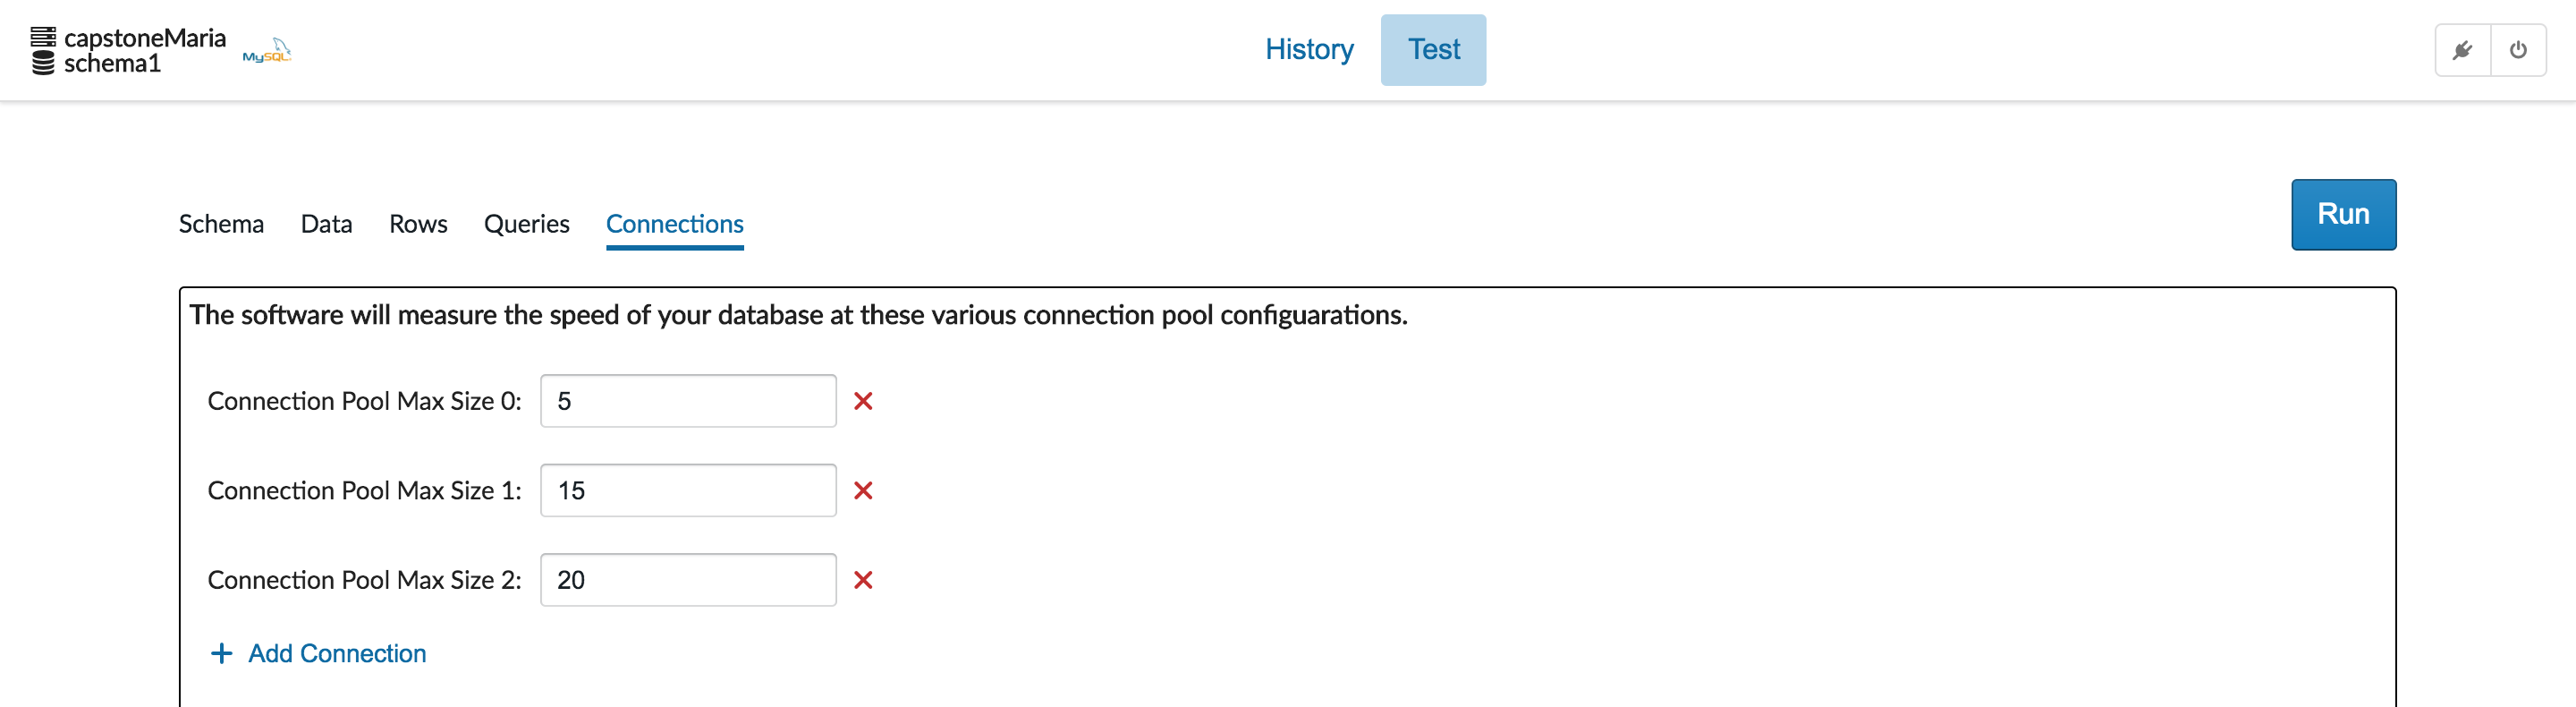
\includegraphics[width=\textwidth]{3-4-2.png}
		\caption{Max connection pool GUI }
		
	\end{figure}
	
	The max connection pool size simulates the ability for the database to handle multiple concurrent requests from a single server. Developers can specify up to five max connection pool configurations to test their SQL databases at. Figure 17 demonstrates SQLitmus's max connection pool configurations GUI.
	
	\subsection{ Running a test}
	
	\begin{figure}[H]
		\centering
		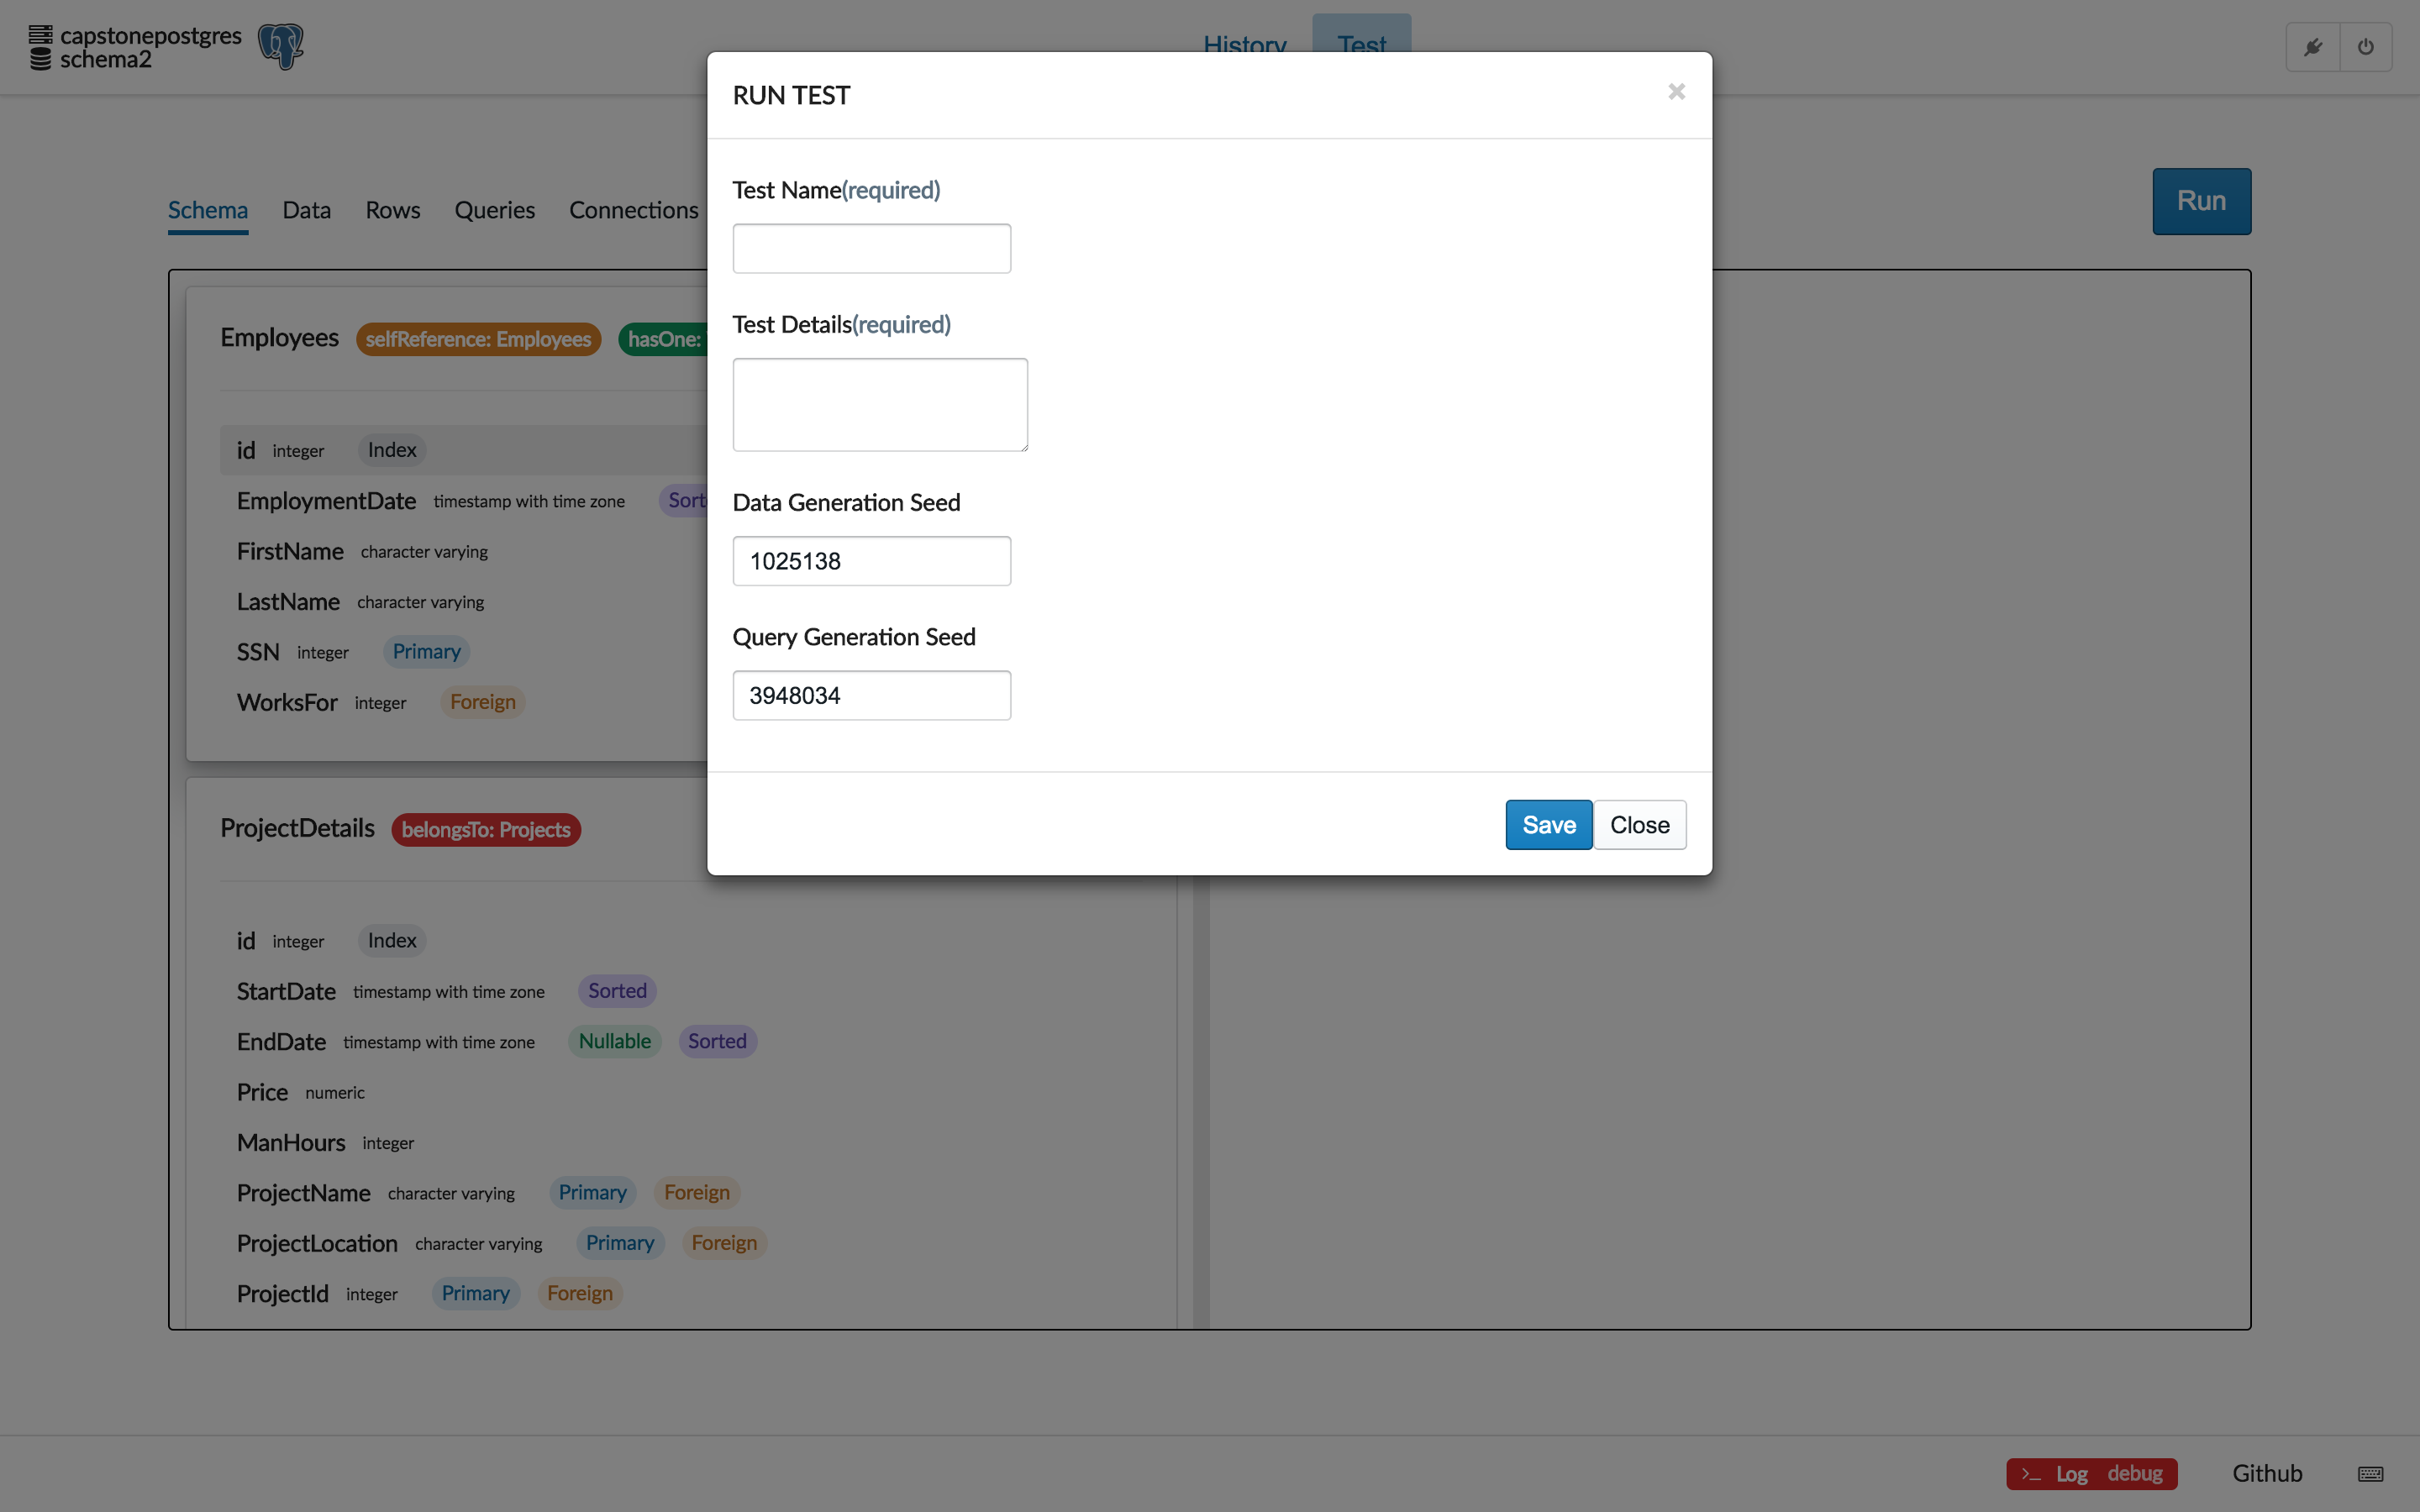
\includegraphics[width=\textwidth]{3-5.png}
		\caption{ Test running modal and its available parameters }
		
	\end{figure}
	
	After the configurations are complete, SQLitmus allows developers to specify separate Data and Query Generation seeds. Each seed deterministically generates the type of data and queries used in the test. This affords developers the option to test multiple databases, or repeat the same test on the same database using the exact same set of data and queries. The seeds are also separated so that developers are able to generate the exact same set of data but test the data-set using a different set of randomly generated queries to account for the chance that the randomly selected queries were "lucky".
	
	Figure 18 displays the how test parameters can be configured on the test running modal.
	
	\subsection{ Data Management}
	
	After all the performance testing is complete, developers still require a simple and effective way of managing their performance analysis results. While the data can simply be exported to other tools for data visualization purposes, the author of SQLitmus believes that a full feature data management solution optimized for visualizing query response time trends should still be made available within SQLitmus itself. This provides an additional layer of convenience for developers.
	
	\subsubsection{History of test records}
	
	\begin{figure}[H]
		\centering
		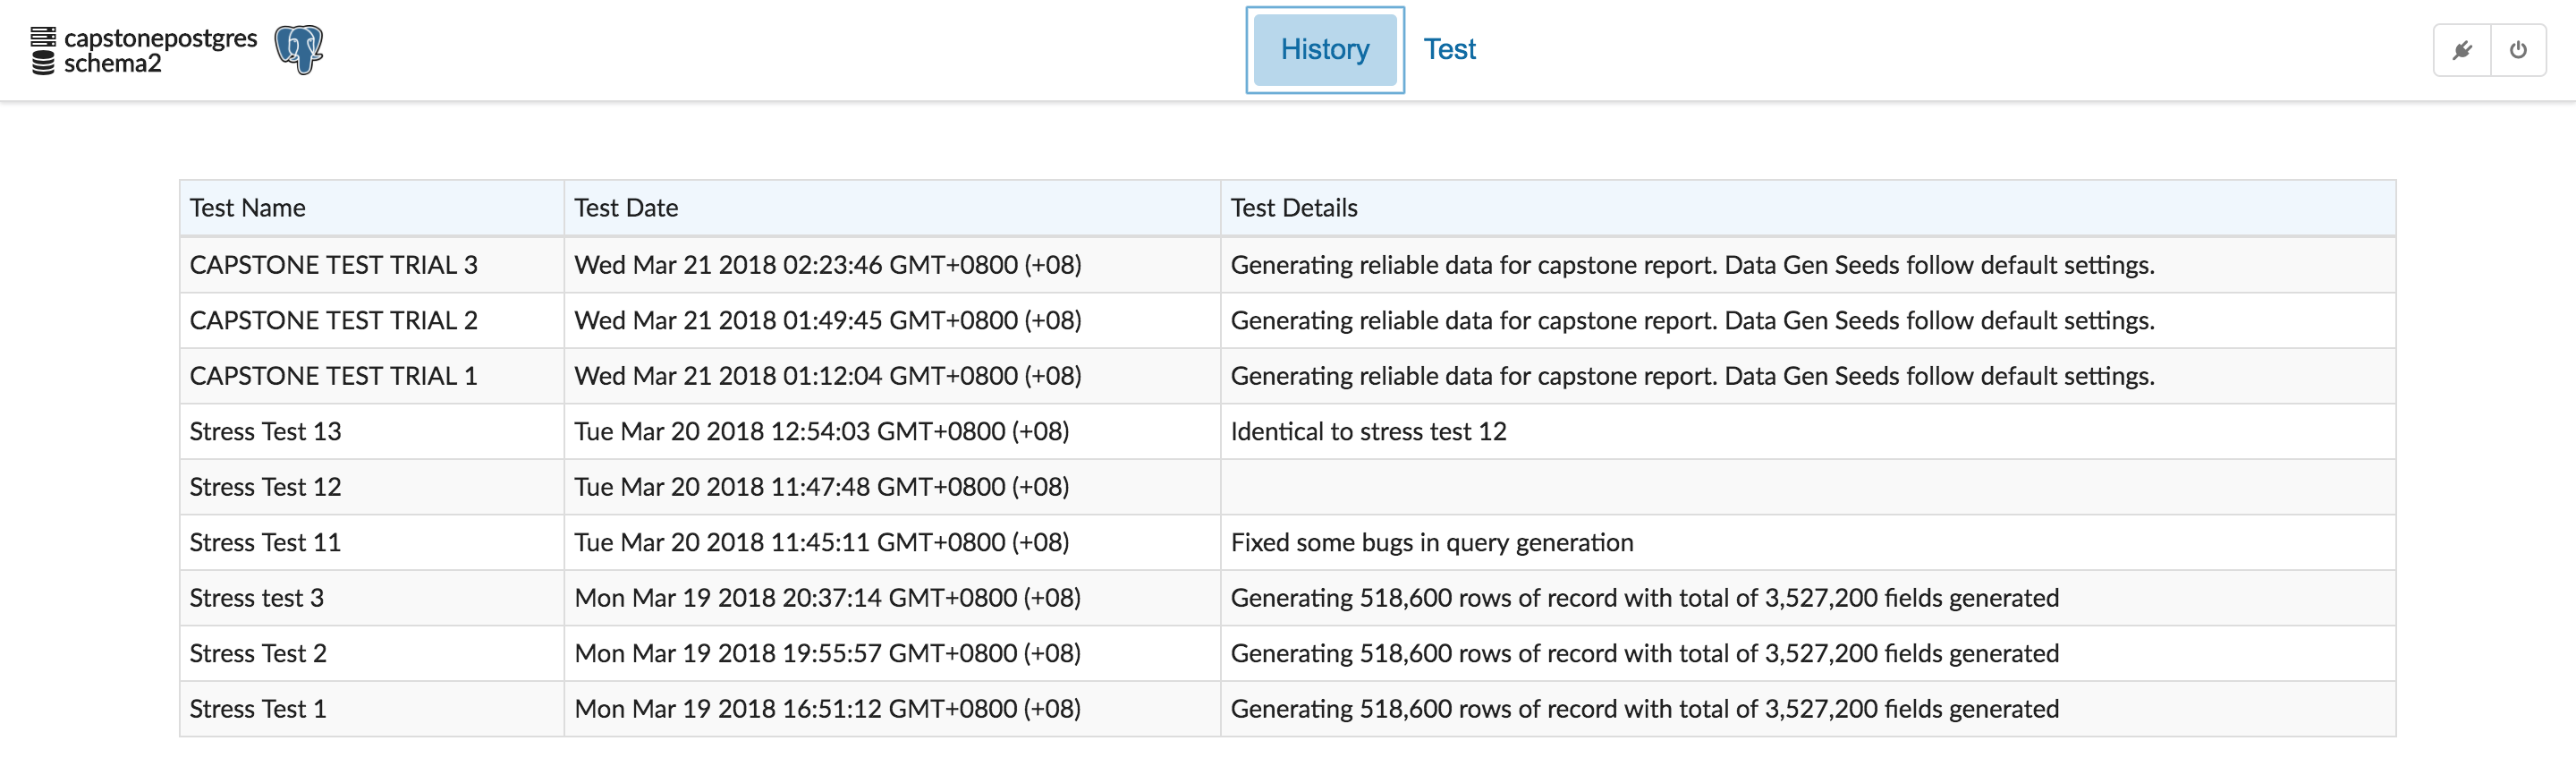
\includegraphics[width=\textwidth]{3-6-1.png}
		\caption{History of test records }
		
	\end{figure}
	
	SQLitmus stores a history of all performance analysis records that users have conducted on a database level. The history is sorted in reverse chronological order as seen in Figure 19 above.
	
	\subsubsection{ Data Visualization}
	
	\begin{figure}[H]
		\centering
		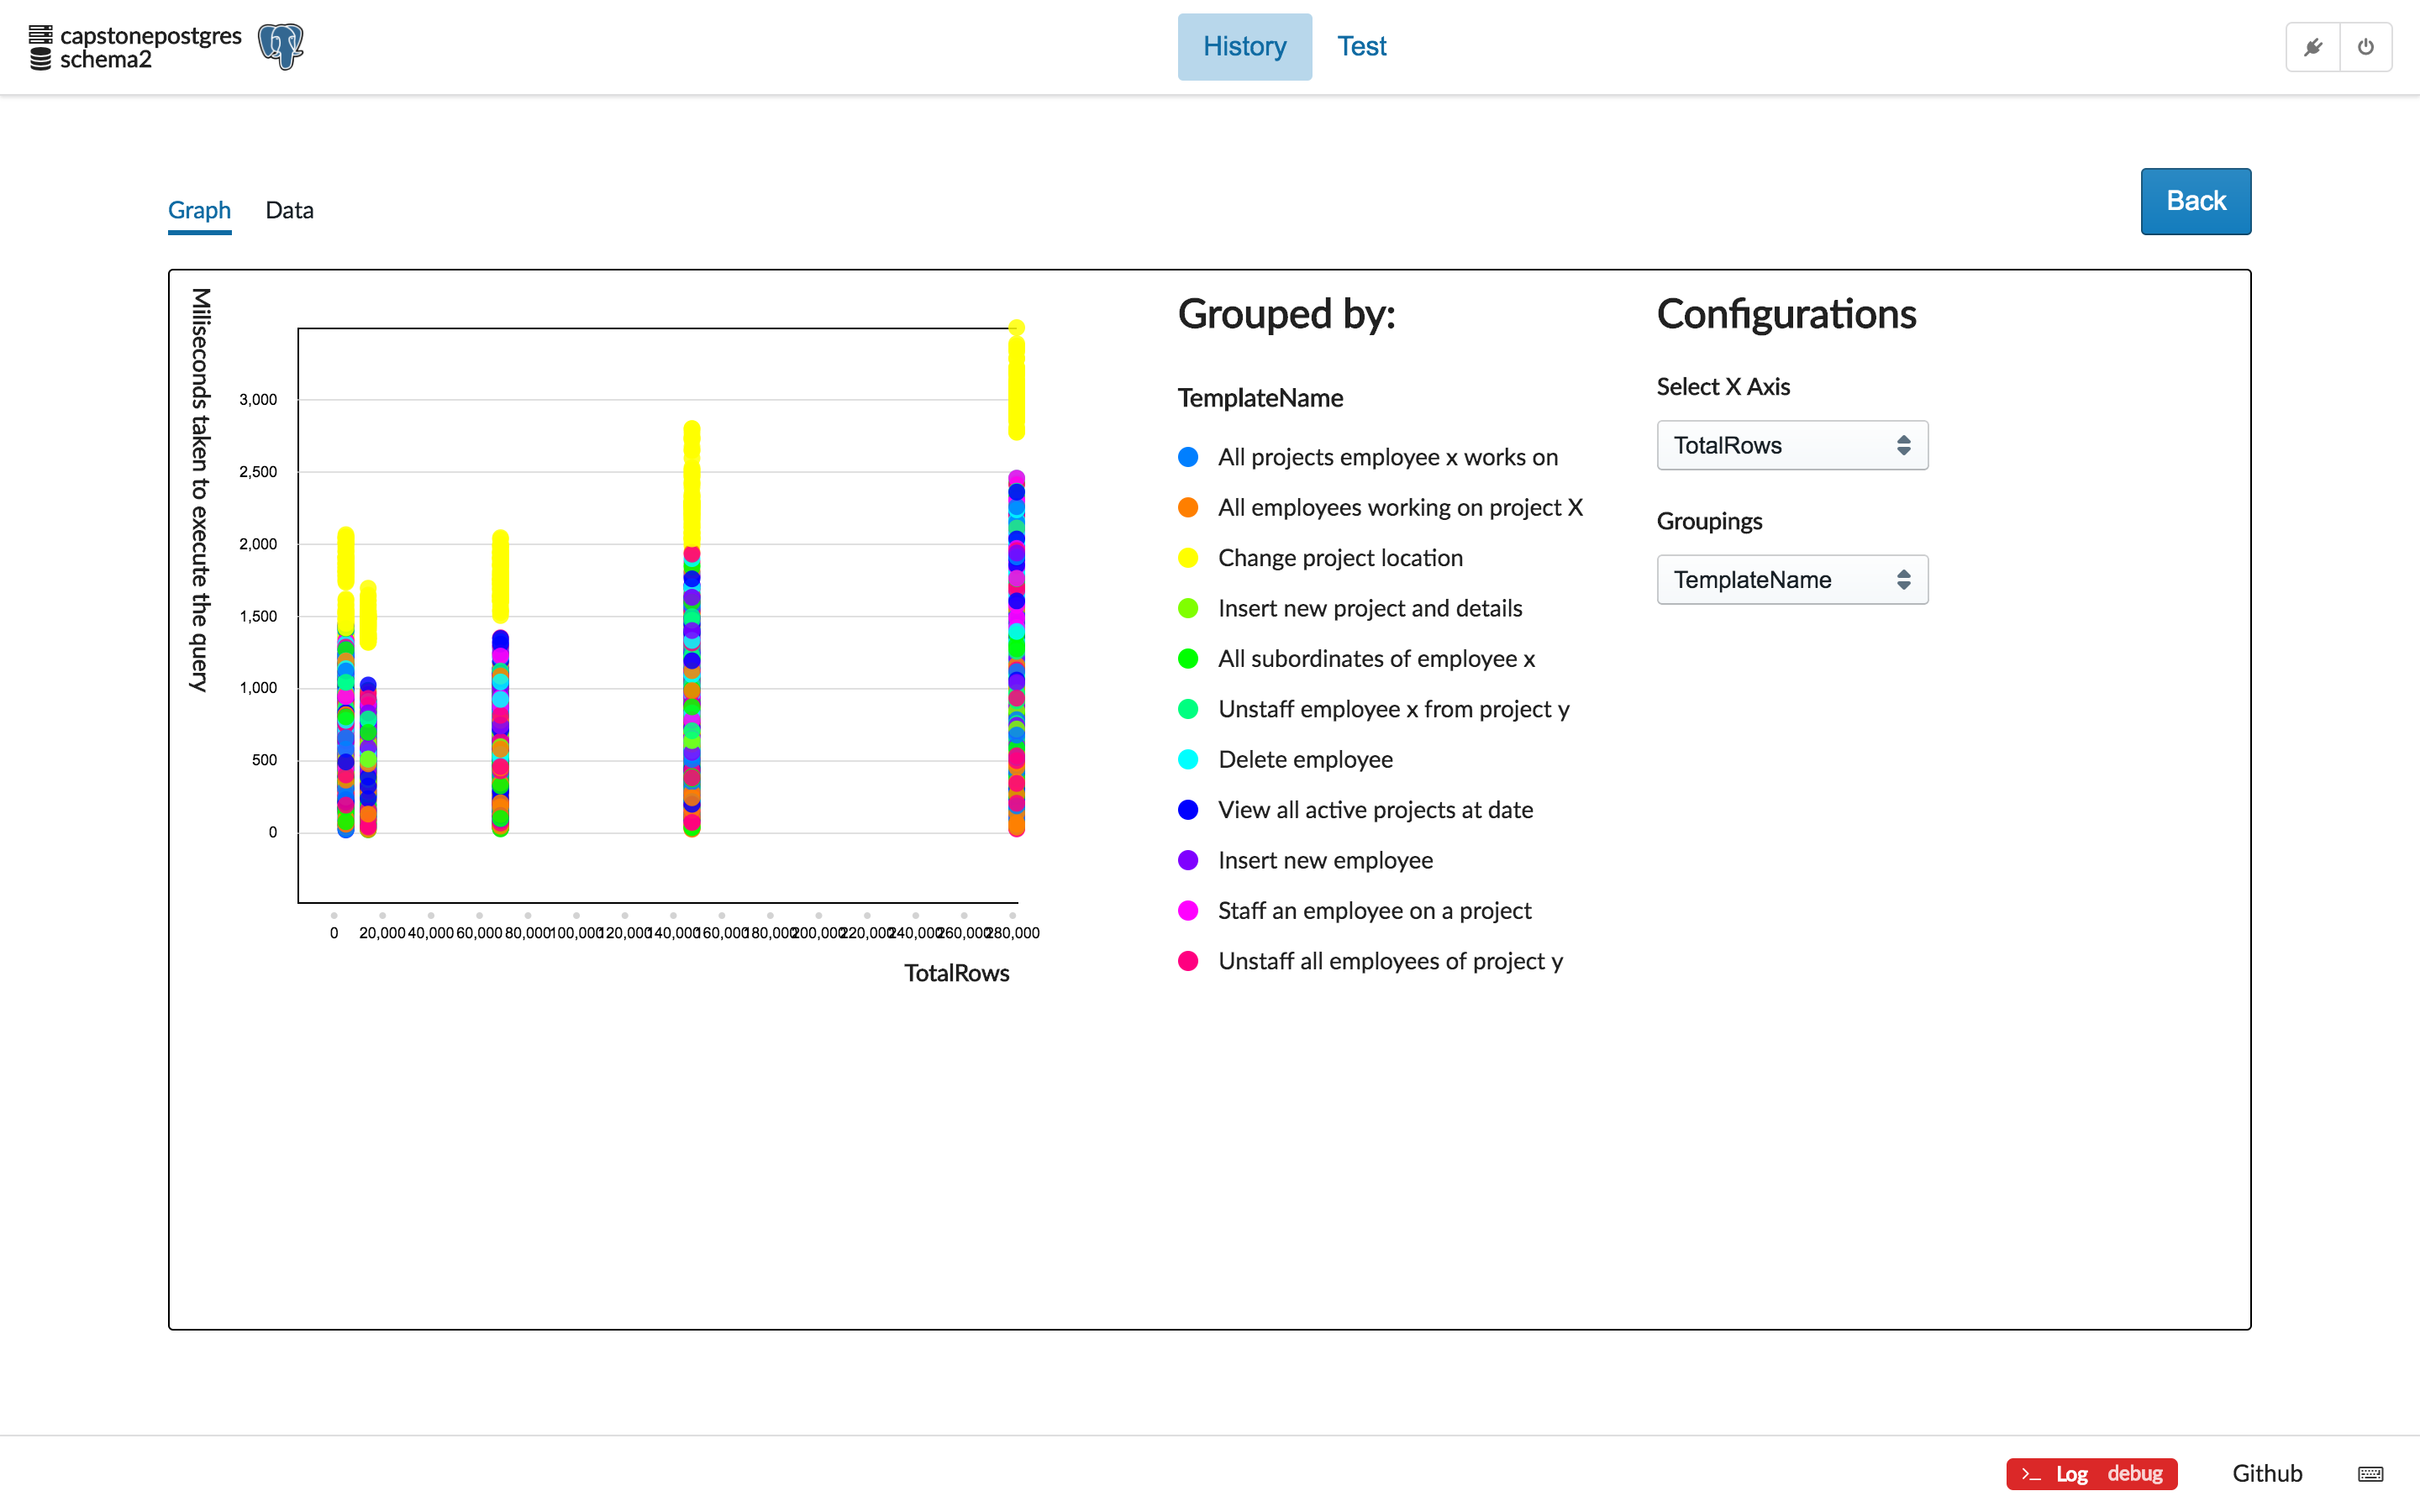
\includegraphics[width=\textwidth]{3-6-2.png}
		\caption{Data visualization module }
		
	\end{figure}
	
	The data visualization component allows developers to identify trends of their database's performance quickly without having to clean or process their data.
	
	Developers are able to investigate their data with a high level of flexibility as the data visualization component allows developers to choose any recorded numerical data for its x-axis and group the data-points using any recorded numerical or string data. Figure 20 demonstrates how the data visualization module can be used to investigate trends.
	
	The color palette was selected using Hue Separation Lightness (HSL) values to ensure that they are visibly distinct from one another. The graph axes were selected to be the minimum range capable of fitting all recorded values.
	
	The graph and legend was developed through using the react-easy-graph library and the colour selection algorithm was taken from Stack Overflow \footnote{https://stackoverflow.com/questions/10014271/generate-random-color-distinguishable-to-humans}.
	
	\subsubsection{ Data filtering}
	
	\begin{figure}[H]
		\centering
		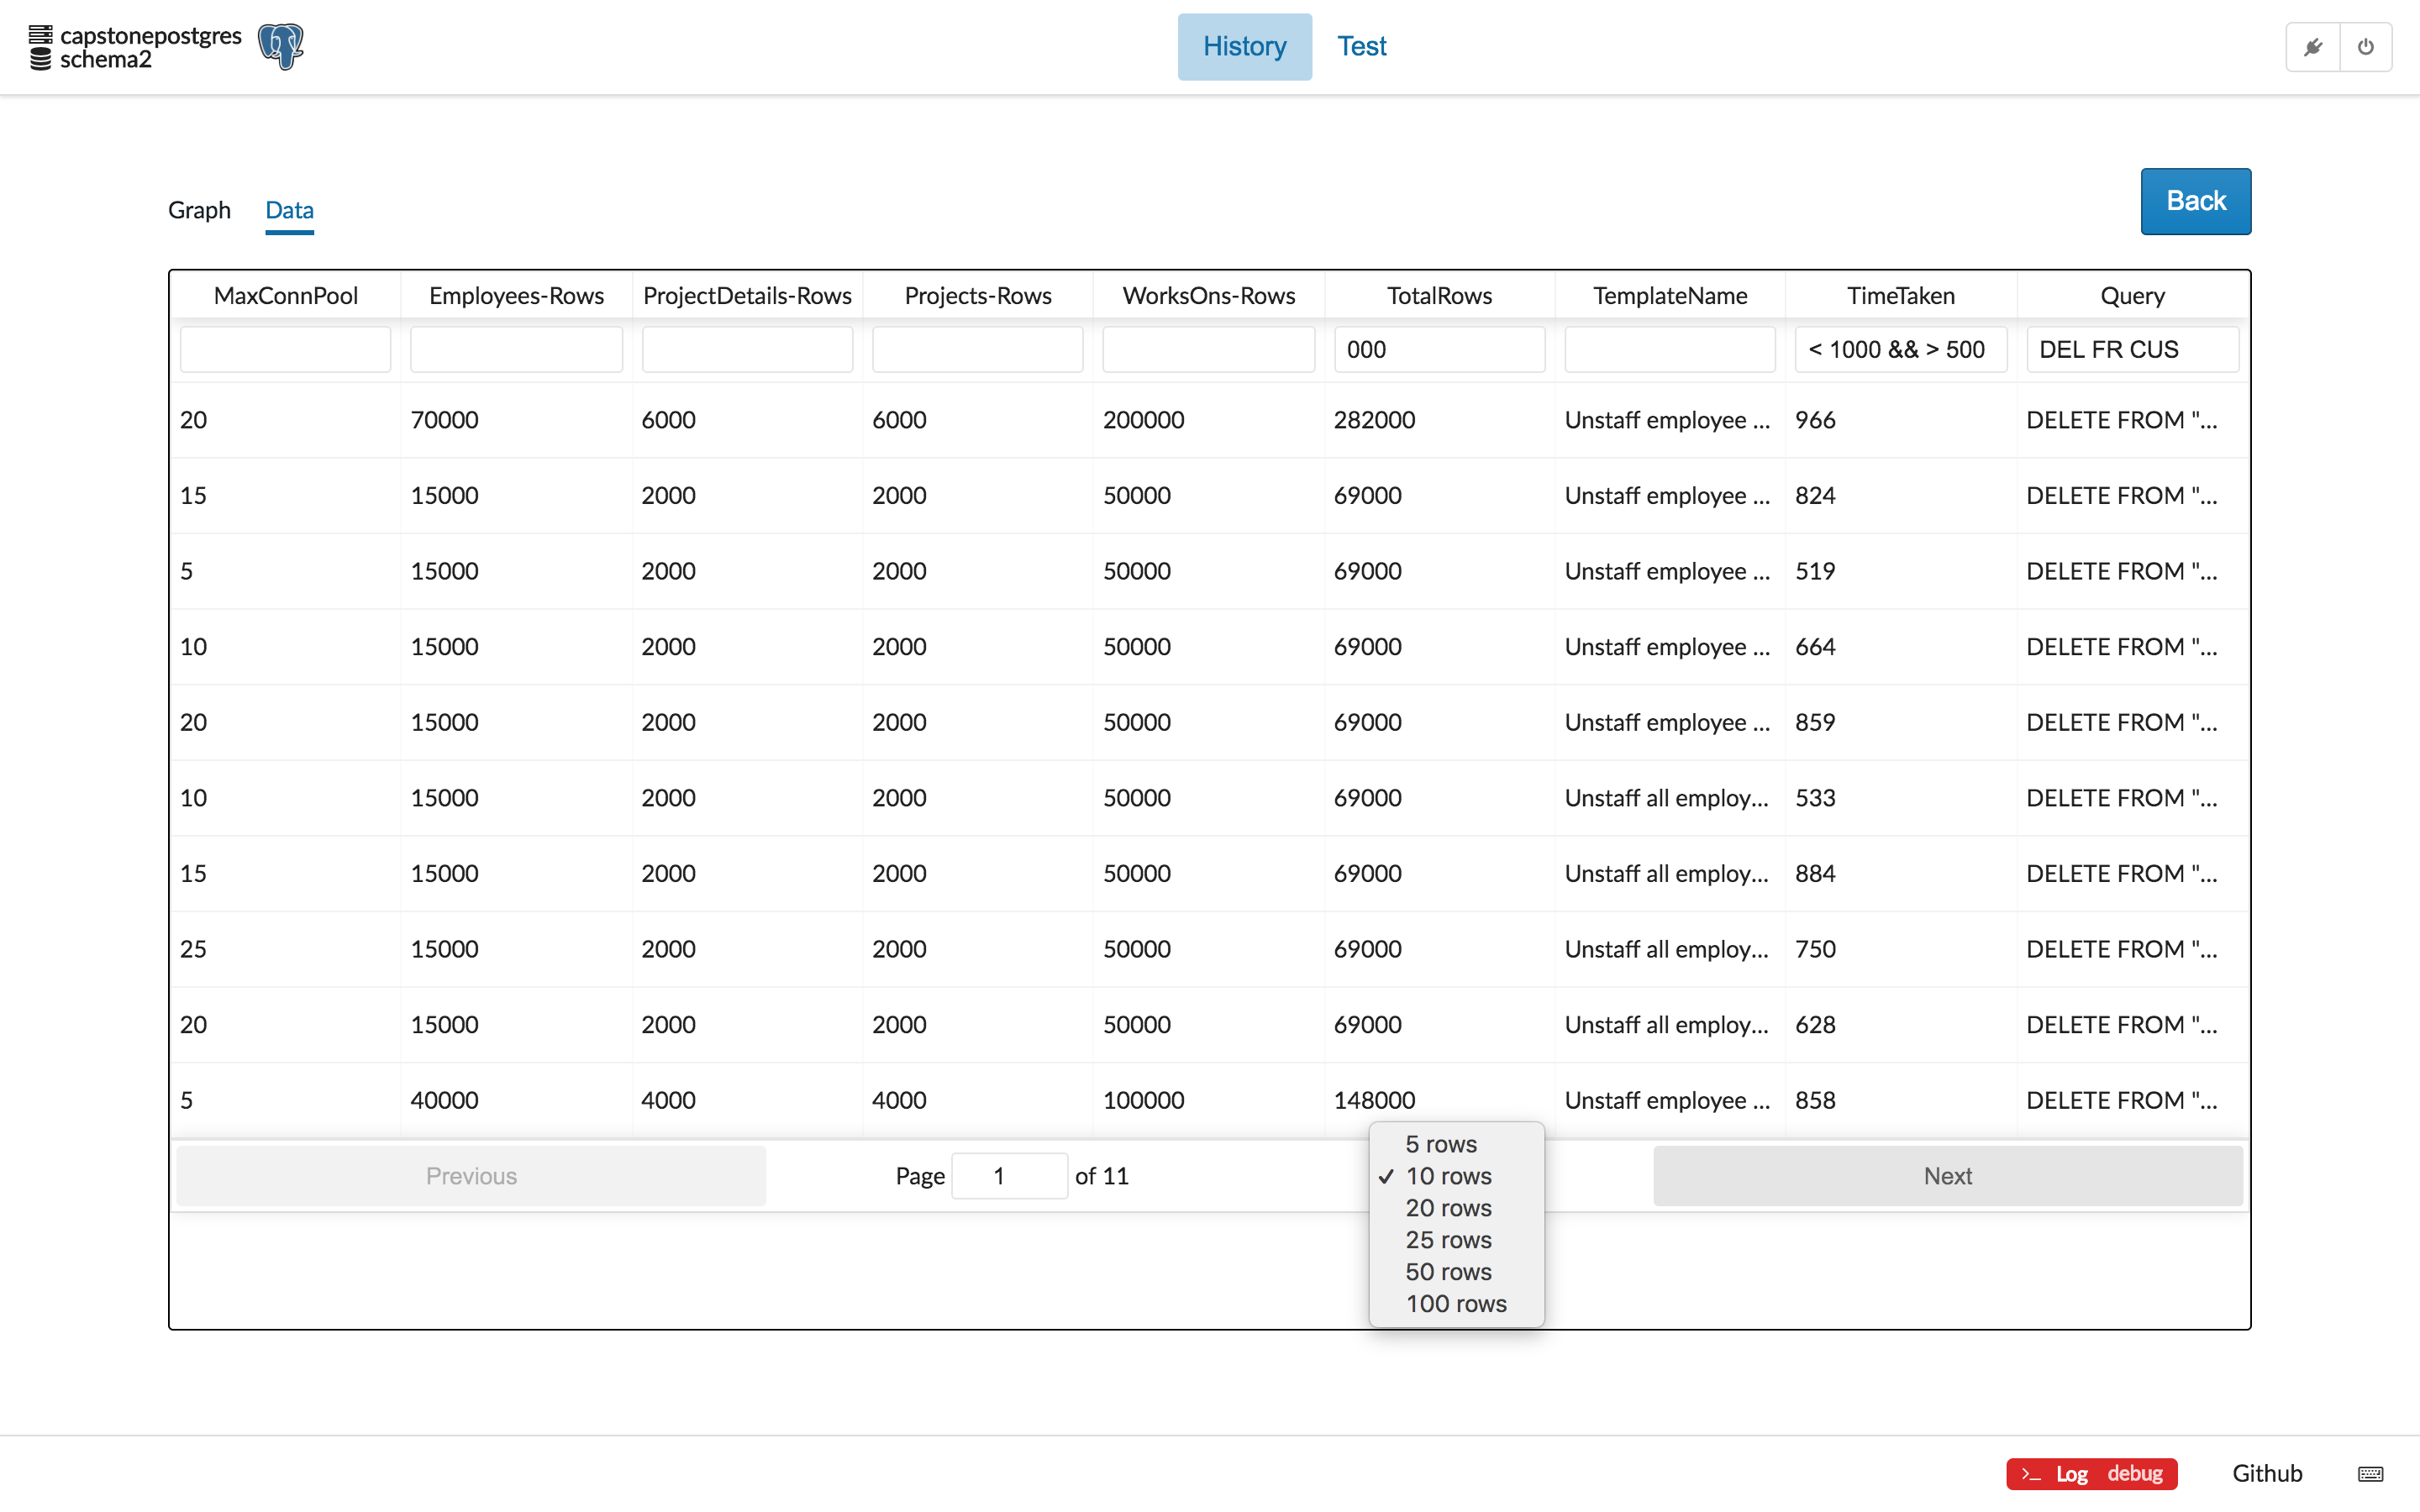
\includegraphics[width=\textwidth]{3-6-3.png}
		\caption{Data filtering module }
		
	\end{figure}
	
	The data filtering component (displayed in Figure 21) provides a way for developers to filter down the the large data-set that they are working with to dig deep into trends of interest.
	
	It allows developers to filter the graphed data-set using a combination of filtering rules specified at a column level. It also uses a powerful filtering engine to afford developers more flexibility.
	
	The word filtering mechanism allows developers to search the string data-sets using intuitive search values. It does not require developers to use complex reg-ex expressions but provides an almost identical level of expressive capability for this intended purpose. It was developed using the help of the match-sorter\footnote{https://github.com/kentcdodds/match-sorter} library.
	
	The number filtering mechanism allows developers to use a combination of intuitive search rules to find their data. The operators supported are:
	\[>=, <=, >, <, =, \&\&, ||\]
	
	\pagebreak
	\section{ Designing a robust test for SQLitmus }
	
	To demonstrate the capabilities of SQLitmus, a robust pilot study was devised.
	
	\subsection{ Test Schema}
	
	\begin{figure}[H]
		\centering
		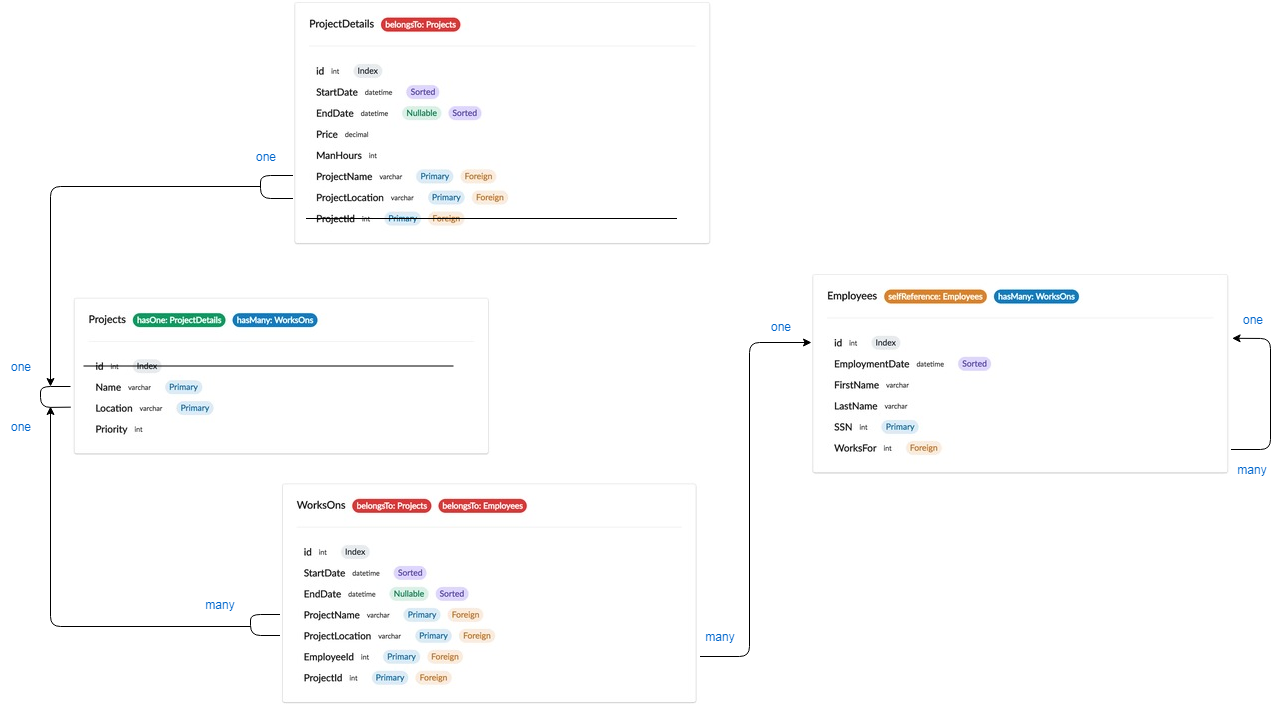
\includegraphics[width=\textwidth]{4-1.png}
		\caption{Test Schema for pilot study }
		
	\end{figure}
	
	The selected test schema was adapted from a similar study conducted by Houkjaer \cite{Houkjaer:2006}.
	
	The schema proposed by Houkjaer tests SQLitmus for the following capabilities:
	
	\begin{itemize}
		
		\item Generating simple primary keys (Employees.id)
		\item Generating composite primary keys (Projects.Name \& Projects.Location)
		\item Generating self-referential foreign keys (Employees.WorksFor $\xrightarrow{}$ Employees.id)
		\item Generating simple many-to-one foreign keys (WorksOns.EmployeeId $\xrightarrow{}$ Employees.id)
		\item Generating composite one-to-one foreign keys (ProjectDetails $\xrightarrow{}$ Projects)
		\item Generating composite many-to-one foreign keys (WorksOns $\xrightarrow{}$ Projects)
		\item Generating many-to-many relationships (Employees \& Projects through WorksOns)
	\end{itemize}
	While Houkjaer's schema allowed us to conduct a robust pilot study on SQLitmus, minor modifications were made to Houkjaer's schema for various reasons. Figure 23 below detail the modifications made to Houkjaer's schema in our pilot study and their related rationale:
	
	
	\begin{figure}[H]
		\centering
		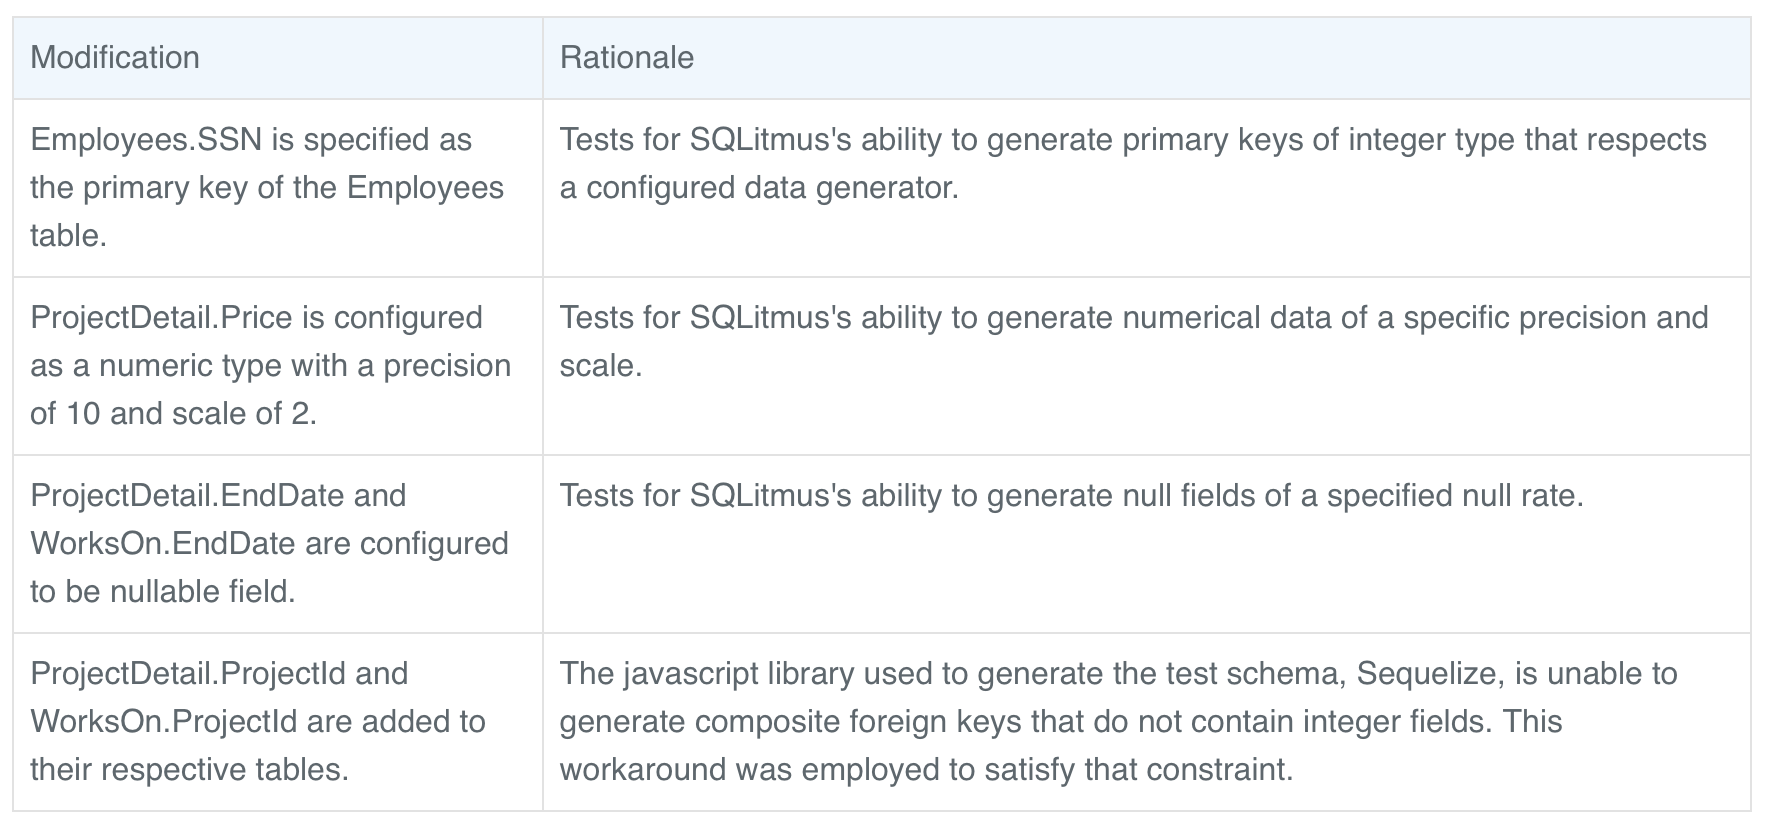
\includegraphics[width=\textwidth]{4-1b.png}
		\caption{Table of modifications and rationale }
		
	\end{figure}
	
	
	
	\pagebreak
	
	\subsection{ Test Queries}
	
	Based on the test schema, a list of query templates were tested for their performance. The list was selected based on transactional workloads that the test schema was likely to face in a production environment.
	
	The following list of workloads were tested for:
	\begin{itemize}
		
		\item Hire a new Employee (Insert new Employee record)
		\item Starting a new Project (Insert new Project record and associated ProjectDetail record)
		\item Staff an employee on a project (Insert WorksOn record)
		\item View all active projects at a specified date
		\item View all employees working on a specific project
		\item View all projects a specific employee is working on
		\item View all direct subordinates of a specific employee
		\item Changing a specified Project record's location (Update a Project record and all associated ProjectDetail and WorksOn records)
		\item Firing an Employee (Delete Employee record)
		\item Unstaff an Employee from a project (Delete WorksOn record)
		\item Ending a project (Delete multiple WorksOn records)
	\end{itemize}
	
	The respective query templates for PostgreSQL and MySQL databases can be found in appendix 1. Despite the differences in the SQL dialects used by both databases, attempts have been made to test both dialects with nearly identical query formats.
	
	\subsection{ Test Configurations}
	
	Figure 24 below specify the row and connection configurations for the test.
	
	\begin{figure}[H]
		\centering
		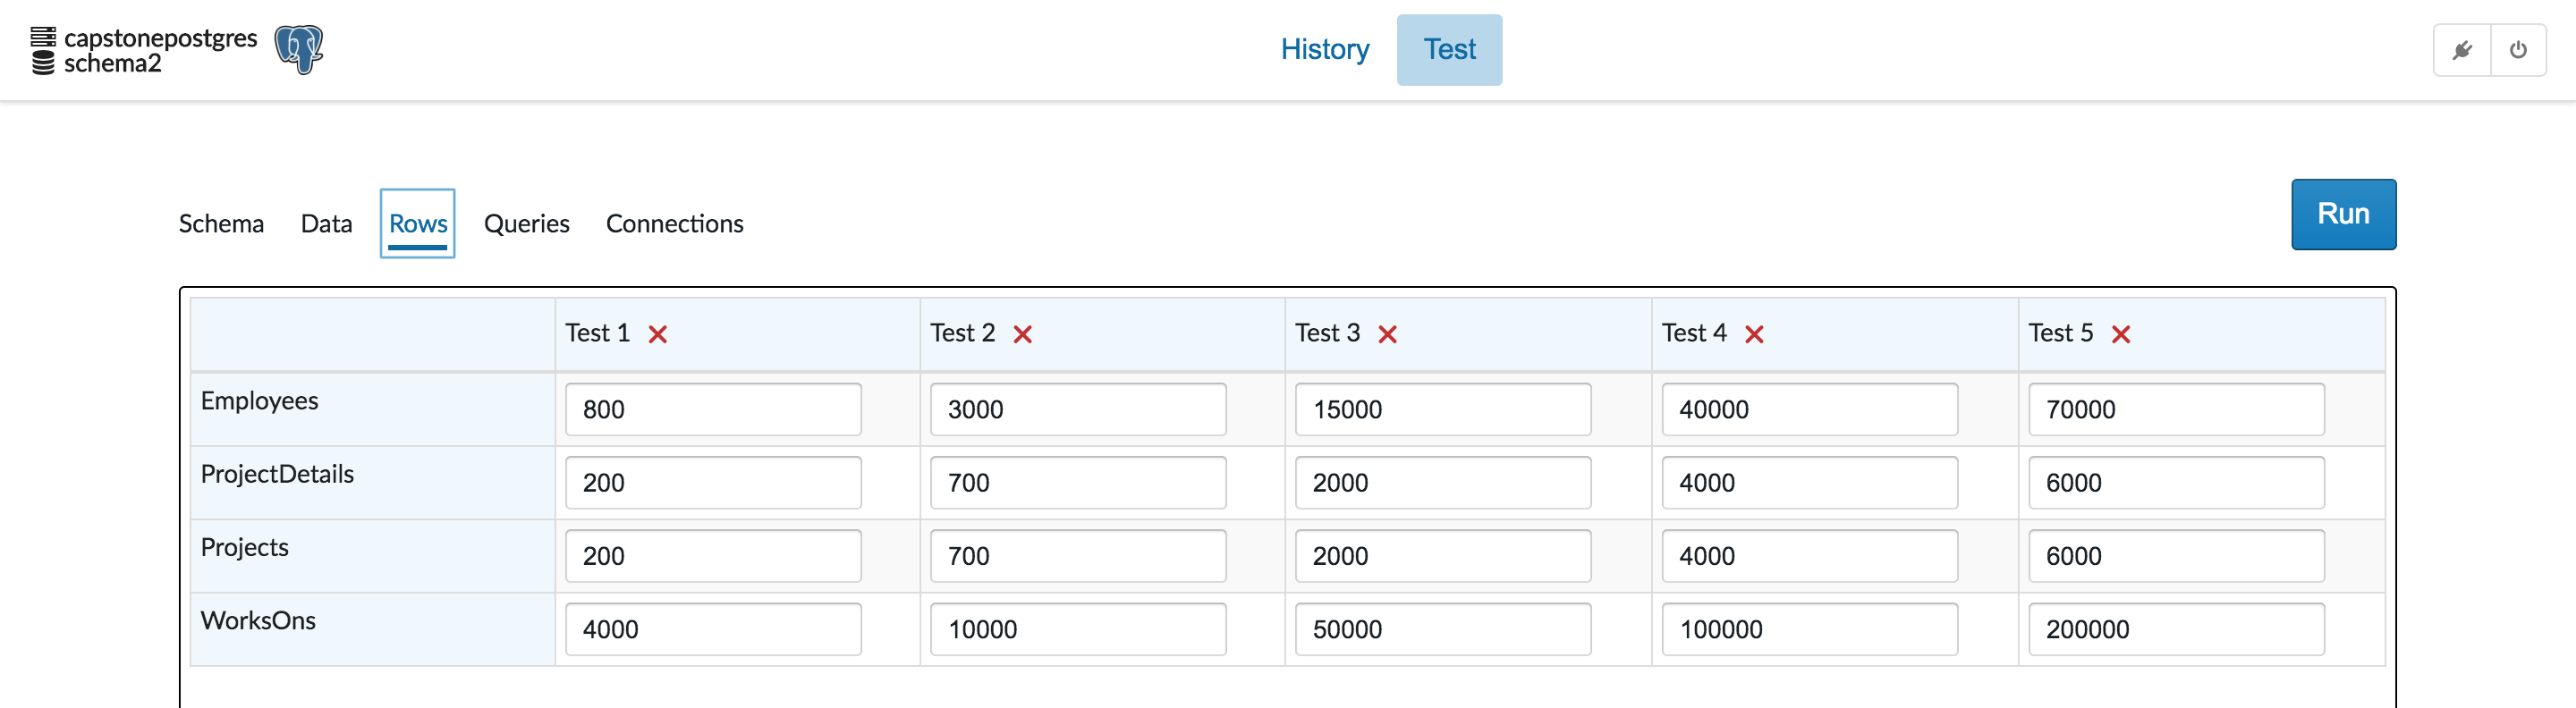
\includegraphics[width=\textwidth]{4-3.png}
		\caption{Test Schema for pilot study }
		
	\end{figure}
	
	The rows selected for the test does not reflect the size of typical company records. Rather, they were selected for to test a typical test data generation workload that the target users of SQLitmus are likely to generate. The above specifications generates a total of 518,600 rows and 3,527,200 fields of data.
	
	\begin{figure}[H]
		\centering
		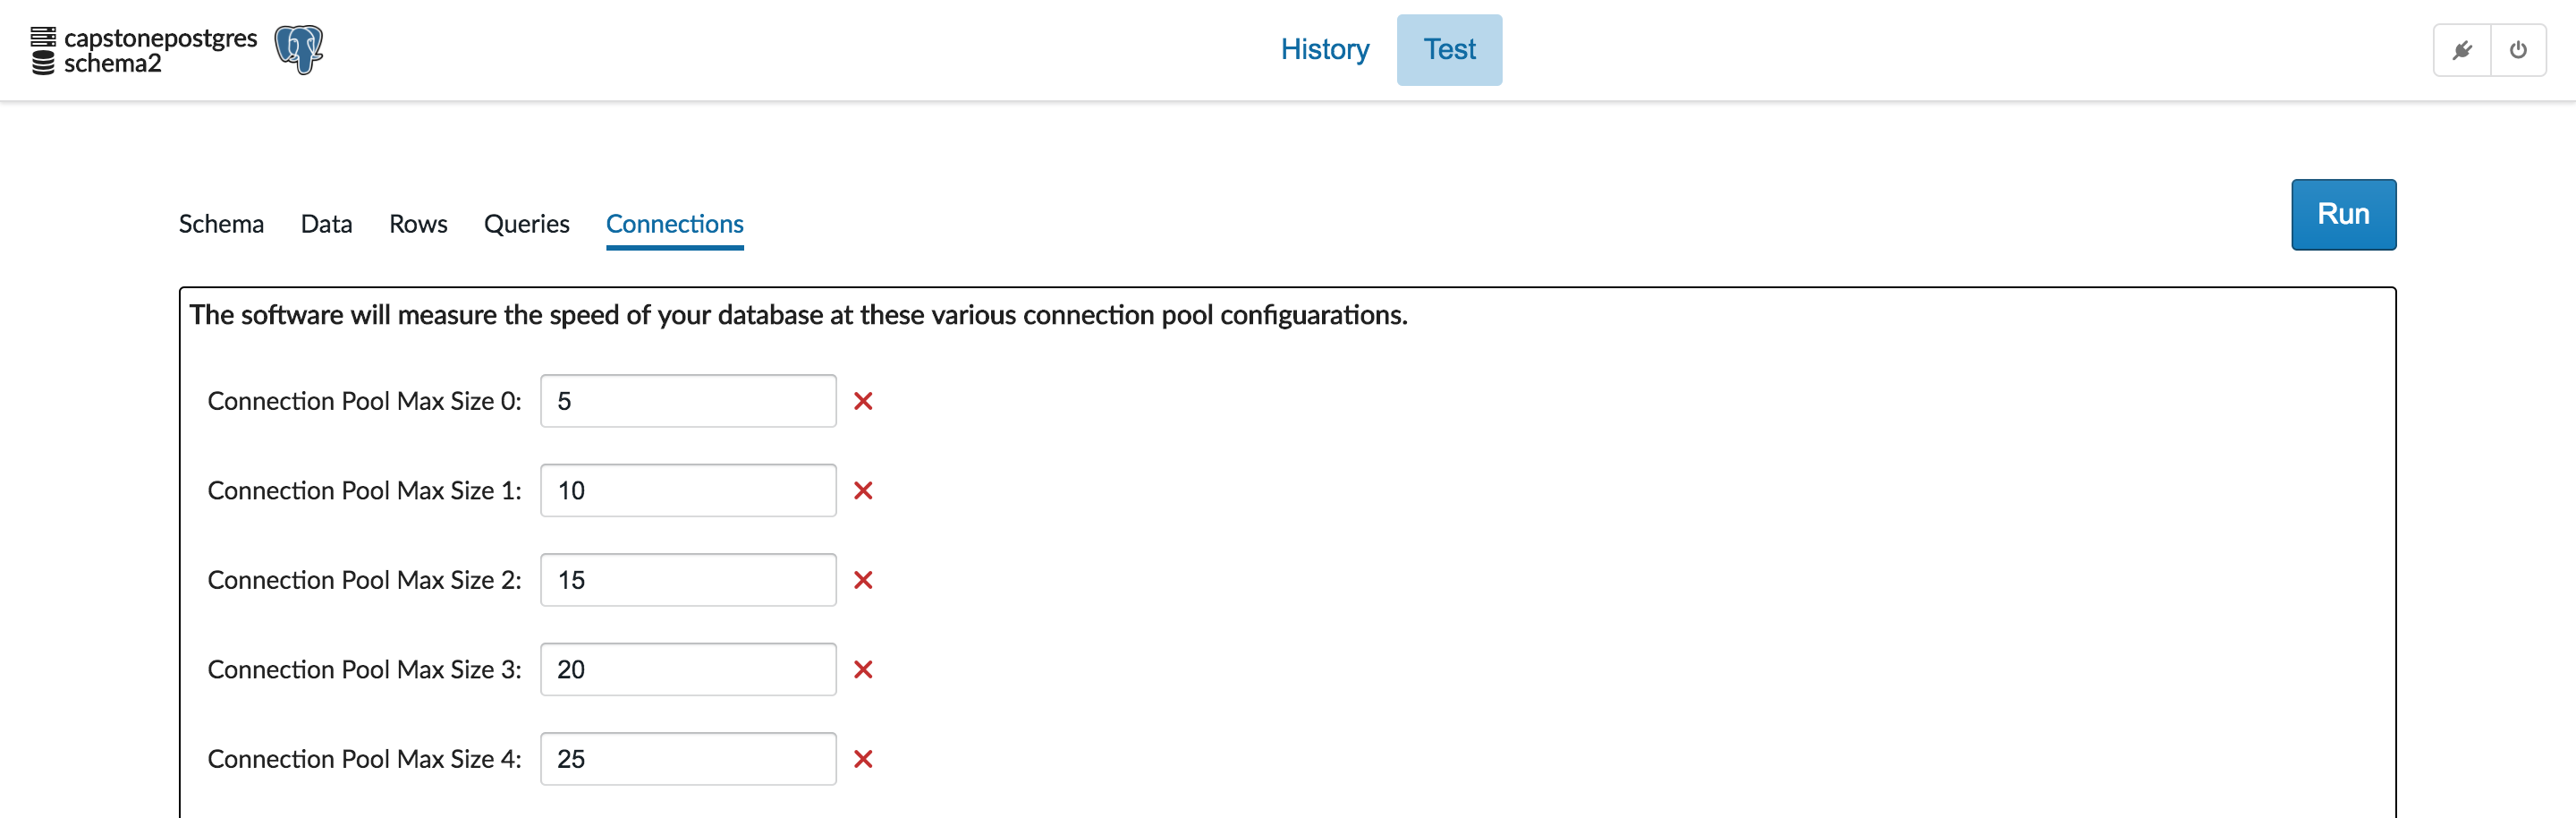
\includegraphics[width=\textwidth]{4-3b.png}
		\caption{Test Schema for pilot study }
		
	\end{figure}
	
	Similar to the row configurations, the max connection pool configurations displayed in Figure 25 were also selected to represent a typical connection pool workload that an average SQLitmus user is likely to test for. 
	
	\section{ Pilot Study}
	
	The pilot study ran SQLitmus against three databases: MySQL, PostgreSQL, and MariaDB. All of which were db.t2.micro instances \footnote{with one virtual CPU, 1GB of RAM, and 20 GB of storage} provisioned by Amazon Web Service's Relational Database Service (AWS RDS) . 
	
	Each of the three databases were tested over three trials to test for the reliability of SQLitmus's performance analyses.
	
	
	\clearpage
	\subsection{ Results}
	\begin{figure}[H]
		\centering
		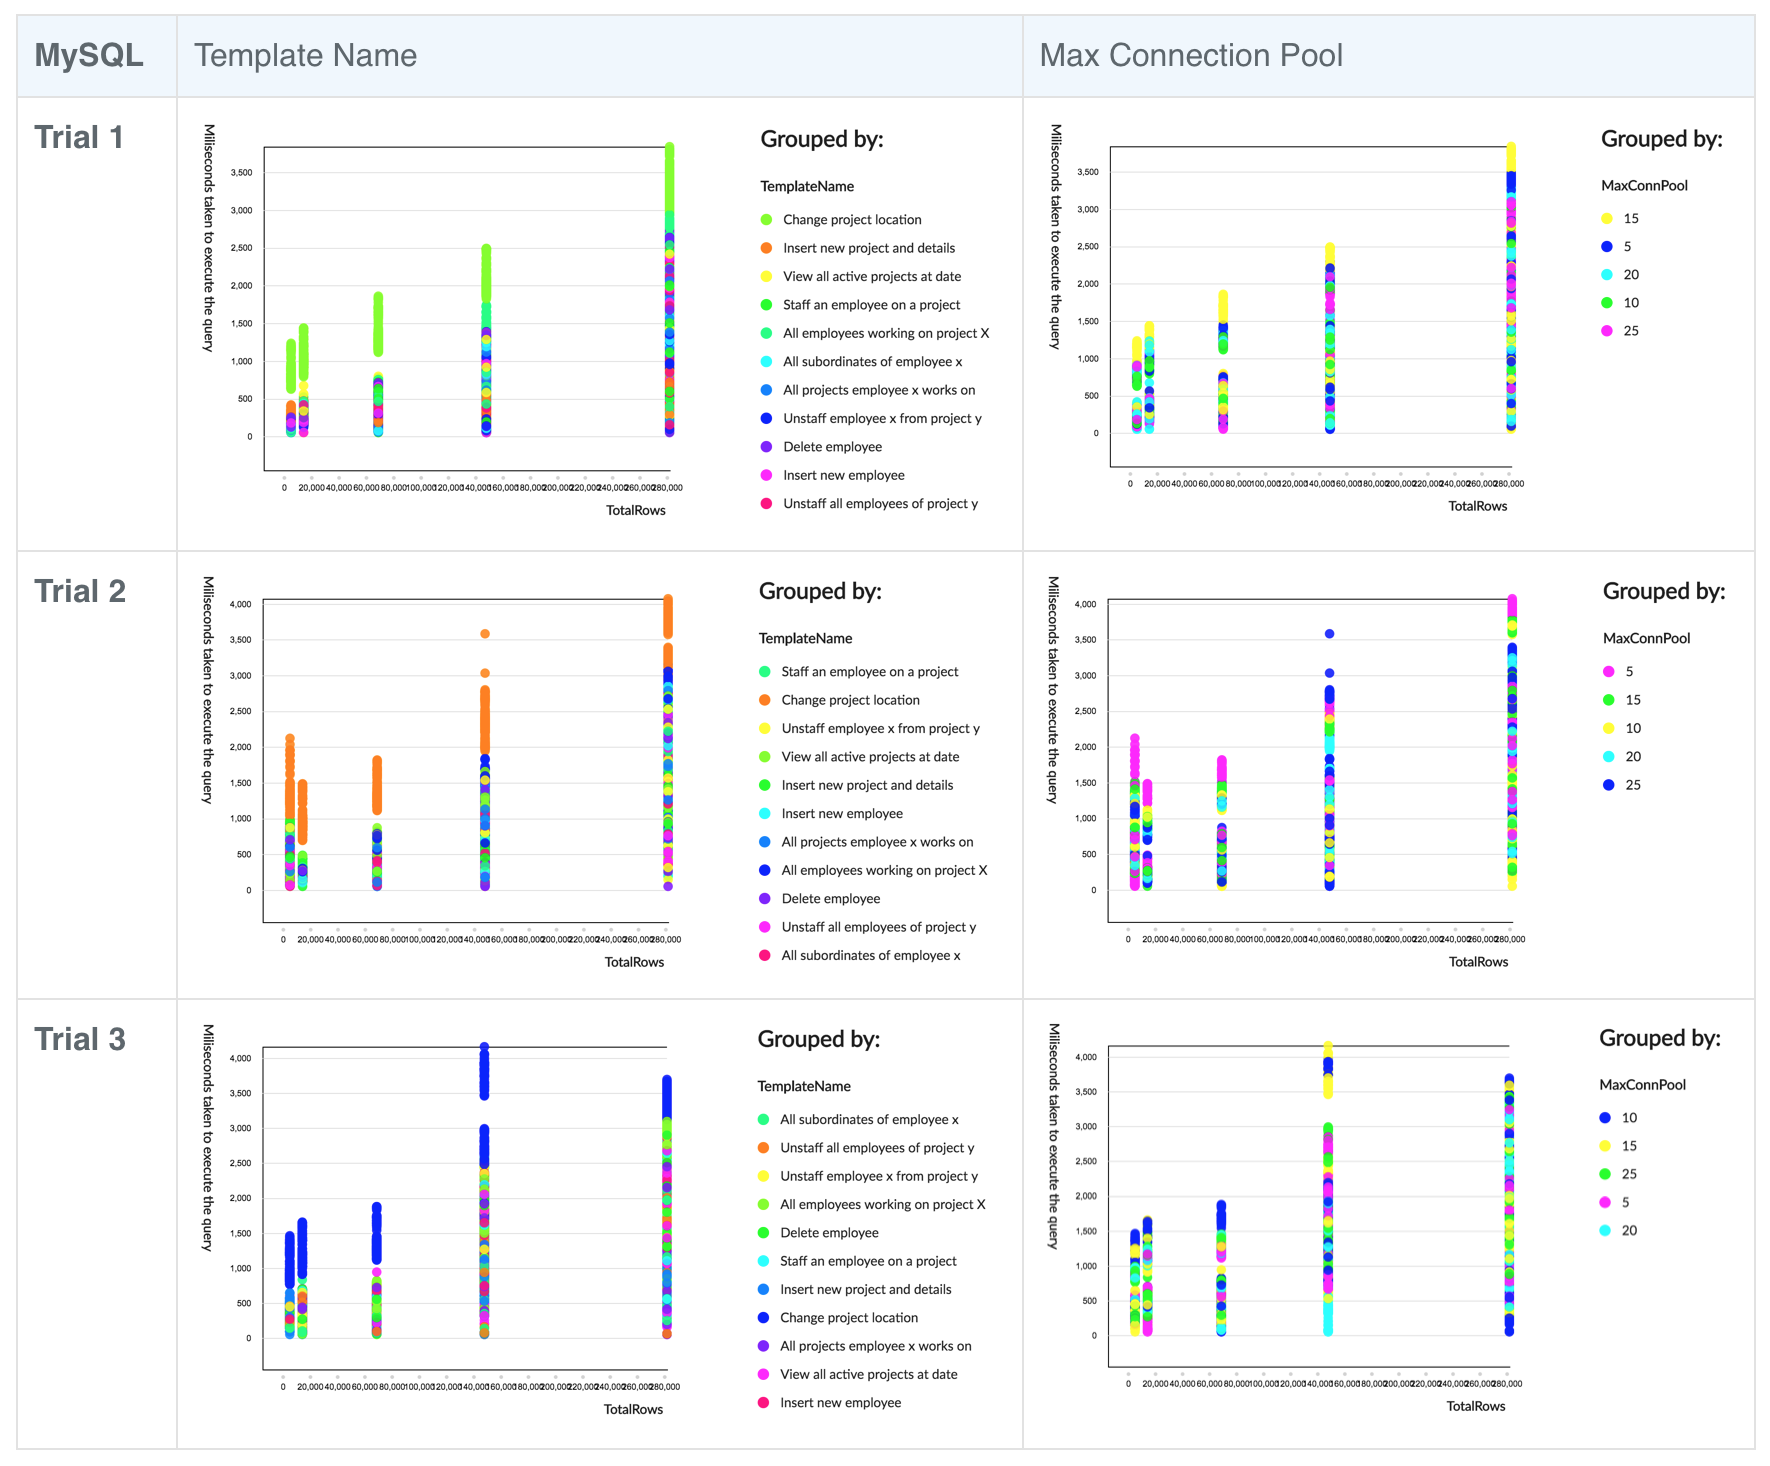
\includegraphics[width=\textwidth]{MySQL.png}
		\caption{Performance results for MySQL }
		
	\end{figure}
	
	\begin{figure}[H]
		\centering
		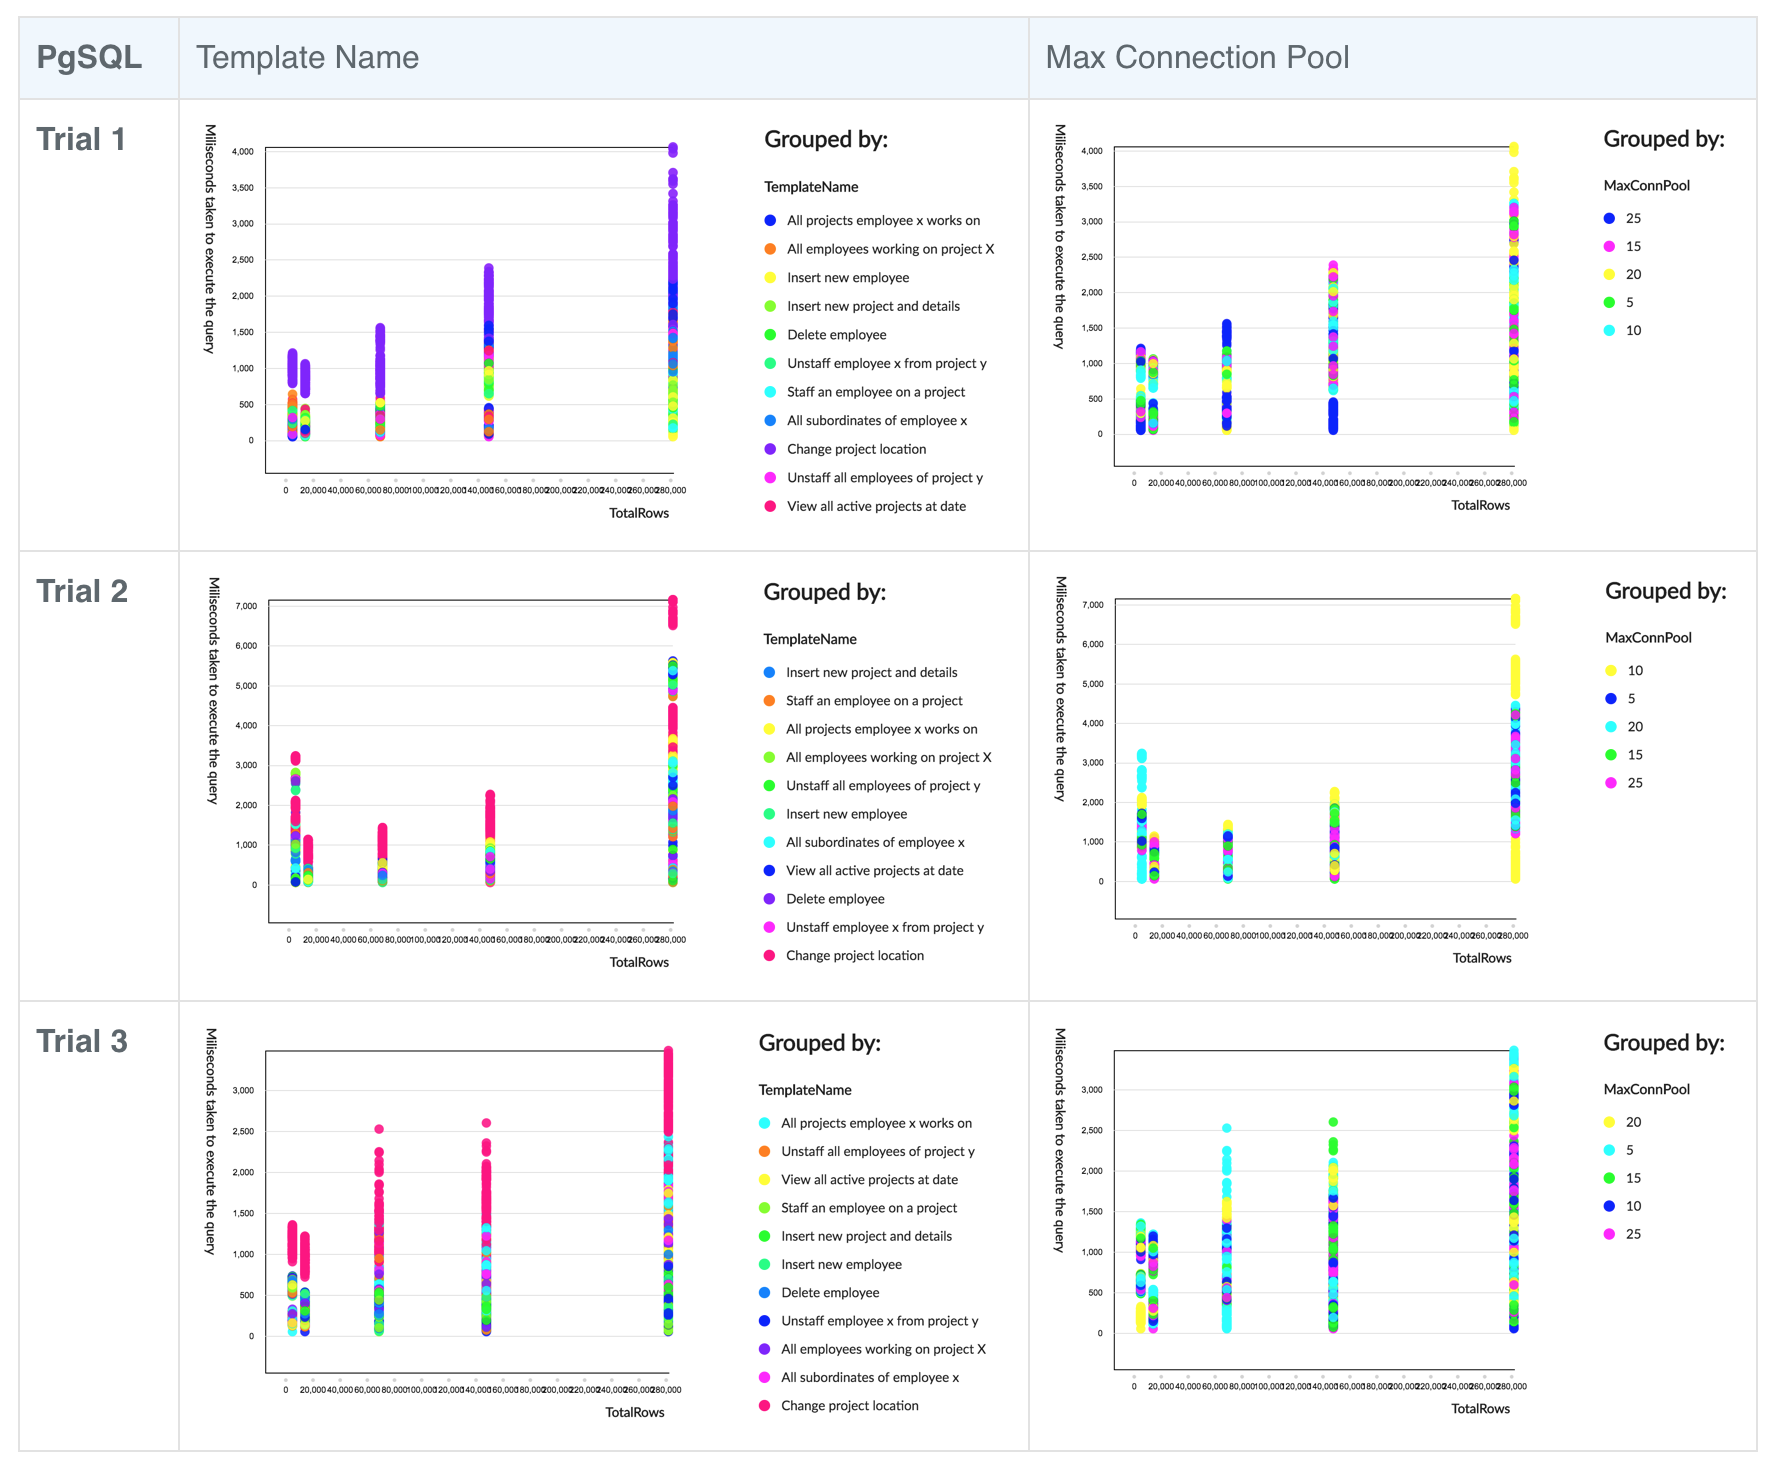
\includegraphics[width=\textwidth]{PgSQL.png}
		\caption{Performance results for PostgreSQL  }
		
	\end{figure}
	
	\begin{figure}[H]
		\centering
		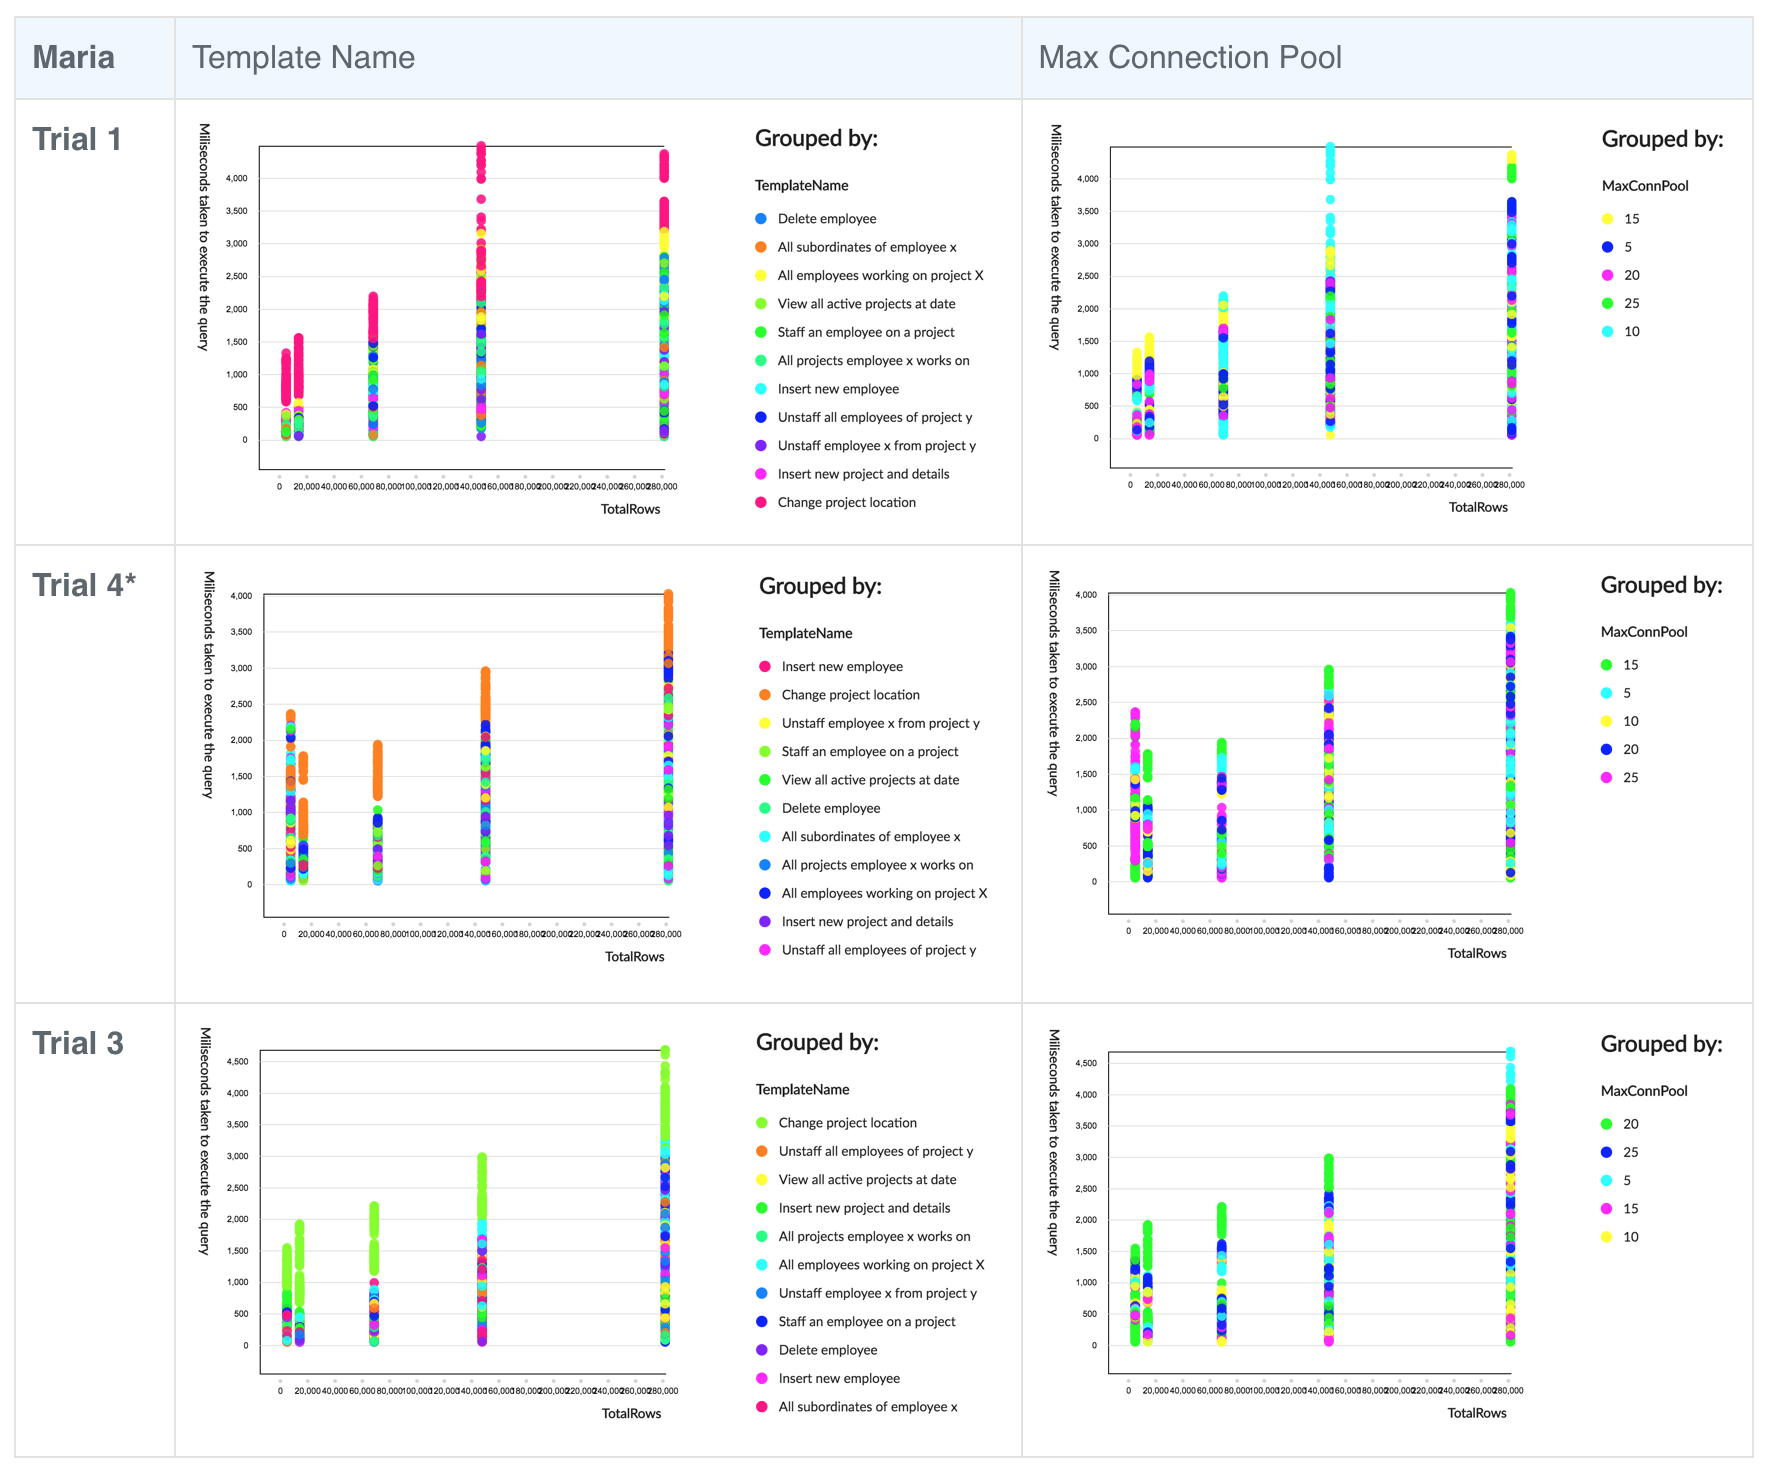
\includegraphics[width=\textwidth]{MARIA.png}
		\caption{Performance results for MariaDB }
		
	\end{figure}
	
	\footnote{Trial 2 results were discarded as the results were anomalous. The computer went into rest mode during the trial and recorded significantly slower readings. The results are available in Appendix 2.}
	
	\clearpage
	
	\subsection{Discussion}
	Let us begin by disambiguating certain terms
	\begin{itemize}
		\item Trial: A single unit of performance analysis conducted by SQLitmus. Each graph in the results section represents an individual trial.
		\item Test: An environment within a trial that SQLitmus runs queries against. Each column of a graph represents a separate test.
	\end{itemize}
	While PostgreSQL's second trial records a maximal response time of 7000 milliseconds,  all of the other eight trials ran recorded a maximal response time of 4000 milliseconds. Firstly, these results demonstrates that performance analyses conducted by SQLitmus are reliable, repeatable, and worthy of discussion.
	
	We observe a clear trend of queries taking a longer time to execute as the size of the database increases. This is a consistent finding across all nine trials. While there are some minor exceptions observed which we may attribute to network instability, \footnote{The tests were conducted through a Wi-Fi connection.} the observed remains an unmistakable trend.
	
	We are also able to observe the relative performances of each type of query. Across all nine trials, we observe that the time taken to change a project's location is often takes the longest time to execute. While there are also queries that often take a short time to execute, such as inserting a new employee, the graph is far too crowded near the bottom for us to yield any possible intelligence. For cases such as these, developers are able to use the data filtering feature.
	
	We also observe no clear trend between the Max Connection Pool Settings and query response time measurements. However, upon visualizing the response times with the Max Connection Pool settings along the X-axis, a faint negative correlation was discovered.
	
	\begin{figure}[H]
		\centering
		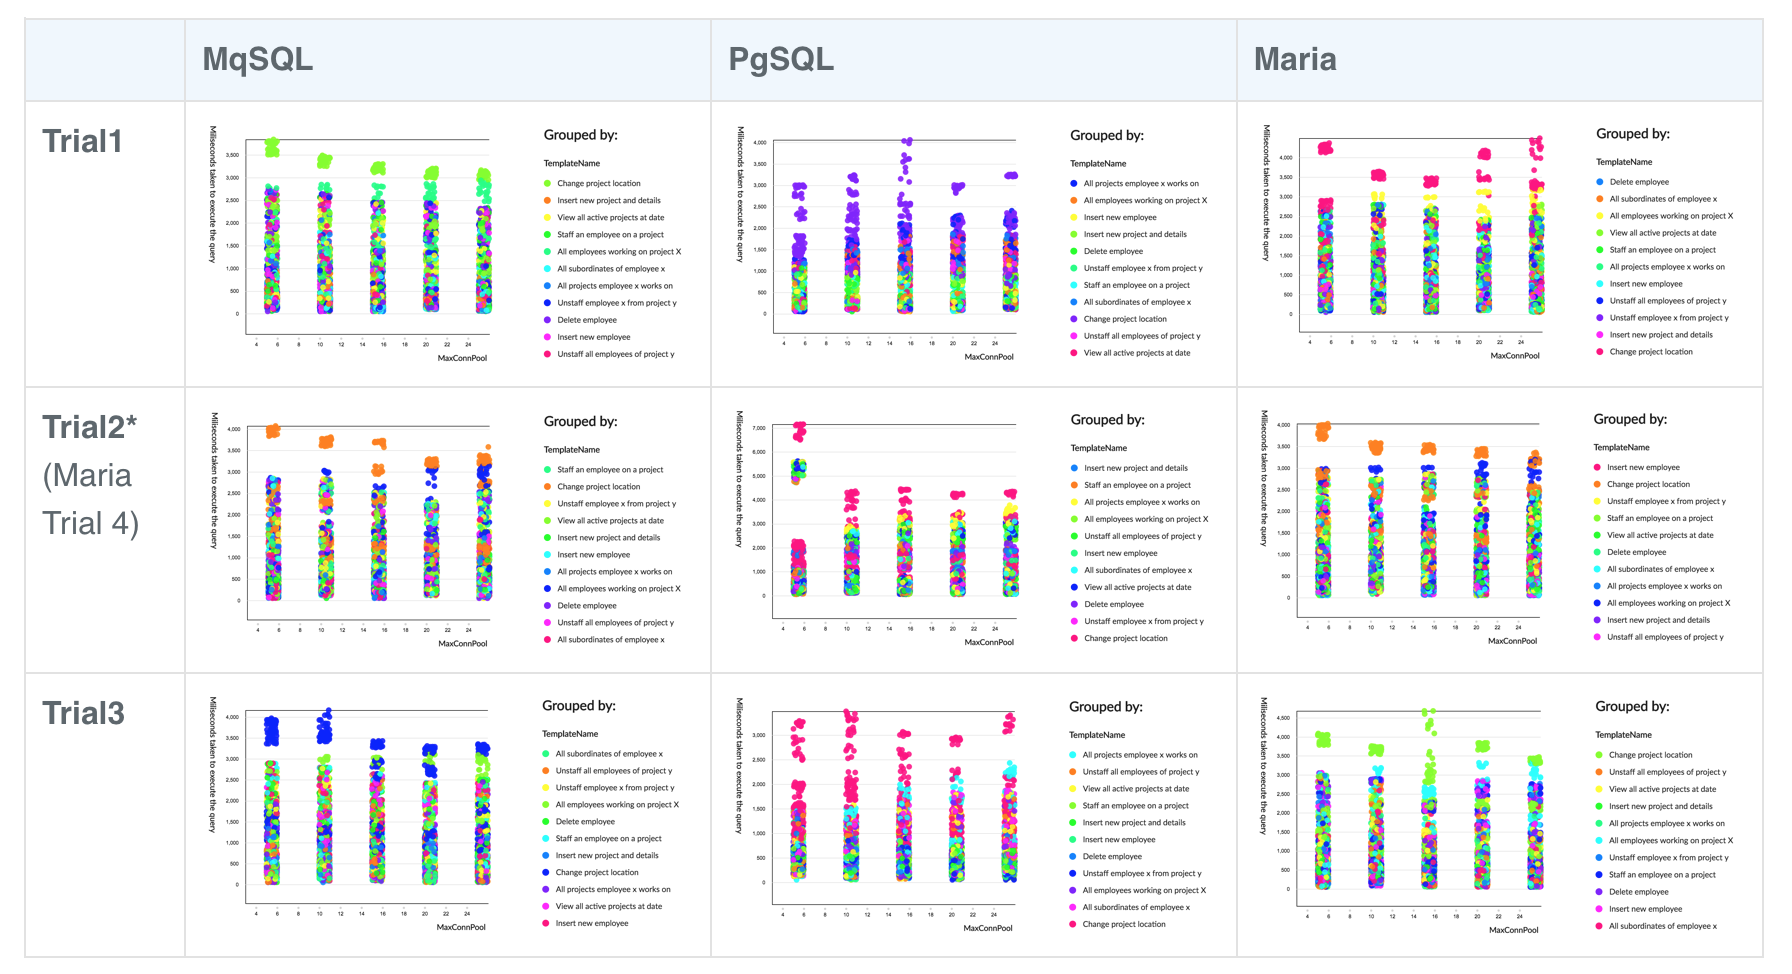
\includegraphics[width=\textwidth]{MCP.png}
		\caption{Using Max Connection Pool as X-axis }
		
	\end{figure}
	
	While these results are not conclusive, a contributing cause could be the poor experimental design. The connection pool settings of: \[5,10,15,20,25\] may not have been values distinct enough to affect the database's performance.
	
	\clearpage
	\section{Summary}
	
	
	
	\subsection{ Limitations}
	
	SQLitmus used many open-sourced libraries to speed up its development. While this is not usually a large concern, SQLitmus is a performance-critical application. To perform more optimally, SQLitmus will have to cut down on the number of libraries used during the data generation process and develop its own components. As it currently stands, SQLitmus is far from being well-tuned and optimized. 
	
	Network instability is a confounding variable that SQLitmus has not been able to completely account for. To minimize the impact of network instability, SQLitmus uses a control query to calibrate query response time measurements. 
	\begin{minted}[bgcolor=light-gray,fontsize=\footnotesize,baselinestretch=1.2,linenos]{mysql}
	SELECT 1;
	--------- Query Response Time Measurement ----
	SELECT 1;
	\end{minted}
	The control query is run before and after measuring any query response time, and the average time taken to run the two control queries is taken as the baseline network instability. SQLitmus then subtracts this baseline value from its respective query response time measurement to minimize the impact of network instability on the recorded results. While it is a simple mechanism, it has drastically improved the quality of performance analyses conducted by SQLitmus.
	
	The results obtained from the pilot test is also limited by the lack of data visualization options provided by the data visualization component.
	
	\subsection{ Future work}
	
	The following issues are being prioritized for SQLitmus:
	\begin{enumerate}
		\item Shifting in-memory workload to disk storage
		\item Faster data generation
		\item Query templates that allow zero cardinality drift for singular inserts and deletes
		\item Better data visualization
	\end{enumerate}
	
	To solve issue 1, SQLitmus is currently exploring the use of flat CSV files for storage. While it is simple to work with csv files, SQLitmus has to tweak its data generation process substantially to ensure that the csv files are created using only a one-time sequential write.
	
	To solve issue 2, SQLitmus is intending to explore the use of algorithms presented by Alexandrov\cite{Alexandrov:2012} and Rabl\cite{Rabl:2013}. These algorithms combined with the logarithmic random access times of the PCG RNG will allow SQLitmus to avoid expensive disk reads. This feature becomes substantially more important if the solution to issue 1 were to be successfully implemented.
	
	To solve issue 3, SQLitmus will also capitalize on the PCG RNG to ensure that every single row of data substituted into the template belongs to an actually existing set of data. SQLitmus will use the query generation seed to select a random index of data to regenerate and use the data generation seed to re-generate the same row that it has generated for the database.
	
	To solve issue 4, SQLitmus will incorporate violin plots into the data visualization component. Violin plots are modified box plots with frequecy distributions plotted on each side. Developers thus gain access to summary statistic visualization which includes quartiles and frequency distributions.
	
	\subsection{ Conclusion}
	
	In this paper we presented SQLitmus, a SQL database performance analysis tool. While it is less sophisticated than other advanced data generators, it is far easier to configure, and features a full-blown GUI for managing all aspects of performance analysis - from data generation, and query generation, to environment configuration, and data management. Performance analysis with SQLitmus is demonstrated to be simple to configure thus the tool is likely to suit the demands of developers of small-to-mid sized applications well. SQLitmus also offers a query templating engine that is more expressive and easier to configure than QGEN\cite{Poess:2004}.
	
	The pilot study of SQLitmus also demonstrated that the tool is capable of generating repeatable and reliable performance analyses of SQL databases. The software recorded clear trends of SQL databases slowing down as their size (amount of data stored) and workload (number of concurrent connections) increased.
	
	Results also revealed performance discrepancies across databases running on identical hardware, data-set, and queries. This shows that SQLitmus can provide developers with intelligence to decide between replaceable databases, queries, and data storage options (eg. time-stamp vs date object).
	
	\printbibliography
	
	\appendix
	
	\section{ Query Templates}
	
	\begin{minted}[bgcolor=light-gray,fontsize=\footnotesize,baselinestretch=1.2,linenos]{mysql}
	
	# Insert new employee (MySQL)
	DELETE FROM Employees WHERE SSN = ${Employees.SSN};
	${BEGIN.DELIMITER}
	INSERT INTO Employees VALUES 
	(null,FROM_UNIXTIME(CEIL(${Employees.EmploymentDate}/1000)),
	${Employees.FirstName},${Employees.LastName}, 
	${Employees.SSN}, ${Employees.RANDROW});
	${END.DELIMITER}
	DELETE FROM Employees WHERE SSN = ${Employees.SSN};
	
	# Insert new employee (PostgreSQL)
	DELETE FROM "Employees" WHERE "SSN" = ${Employees.SSN};
	${BEGIN.DELIMITER}
	INSERT INTO "Employees"  VALUES 
	(DEFAULT, to_timestamp(CEIL(${Employees.EmploymentDate}/1000)),
	${Employees.FirstName},${Employees.LastName}, ${Employees.SSN}, 
	${Employees.RANDROW});
	${END.DELIMITER}
	DELETE FROM "Employees" WHERE "SSN" = ${Employees.SSN};
	
	# Insert new project and details (MySQL)
	DELETE FROM Projects WHERE 
	Name = ${Projects.Name} AND Location = ${Projects.Location};
	DELETE FROM ProjectDetails WHERE 
	ProjectName = ${Projects.Name} AND ProjectLocation = ${Projects.Location};
	${BEGIN.DELIMITER}
	INSERT INTO Projects VALUES 
	(null,${Projects.Name},${Projects.Location}, ${Projects.Priority});
	INSERT INTO ProjectDetails Values (null, 
	FROM_UNIXTIME(CEIL(${ProjectDetails.StartDate}/1000)), 
	FROM_UNIXTIME(CEIL(${ProjectDetails.EndDate}/1000)),
	${ProjectDetails.Price}, ${ProjectDetails.ManHours}, 
	${Projects.Name}, ${Projects.Location},
	(SELECT max(id) id FROM Projects));
	
	
	# Insert new project and details (PostgreSQL)
	DELETE FROM "Projects" WHERE 
	"Name" = ${Projects.Name} AND "Location" = ${Projects.Location};
	DELETE FROM "ProjectDetails" WHERE 
	"ProjectName" = ${Projects.Name} AND "ProjectLocation" = ${Projects.Location};
	${BEGIN.DELIMITER}
	INSERT INTO "Projects" VALUES 
	(default,${Projects.Name},${Projects.Location}, ${Projects.Priority});
	INSERT INTO "ProjectDetails" Values (DEFAULT, 
	to_timestamp(CEIL(${ProjectDetails.StartDate}/1000)), 
	to_timestamp(CEIL(${ProjectDetails.EndDate}/1000)),
	${ProjectDetails.Price}, ${ProjectDetails.ManHours}, 
	${Projects.Name},${Projects.Location}, 
	(SELECT "id" FROM "Projects" ORDER BY id DESC LIMIT 1));
	
	#Staff an employee on a project (MySQL)
	DELETE FROM WorksOns WHERE 
	ProjectName = ${Projects.Name} AND ProjectLocation = ${Projects.Location};
	${BEGIN.DELIMITER}
	INSERT INTO WorksOns VALUES (null,
	FROM_UNIXTIME(CEIL(${WorksOns.StartDate}/1000)),
	FROM_UNIXTIME(CEIL(${WorksOns.EndDate}/1000)),
	${Projects.Name}, ${Projects.Location},
	${Employees.RANDROW},${Projects.RANDROW});
	
	#Staff an employee on a project (PostgreSQL)
	INSERT INTO "WorksOns" VALUES (DEFAULT,
	to_timestamp(CEIL(${WorksOns.StartDate}/1000)),
	to_timestamp(CEIL(${WorksOns.EndDate}/1000)),
	${Projects.Name}, ${Projects.Location},
	CEIL(random()*${Employees.numRows}),
	CEIL(random()*${Projects.numRows}));
	
	#View all active projects at date (MySQL)
	SELECT Name, Location, StartDate, EndDate, Price, ManHours 
	FROM ProjectDetails JOIN Projects 
	ON Projects.Name=ProjectDetails.ProjectName 
	AND Projects.Location=ProjectDetails.ProjectLocation
	WHERE StartDate < FROM_UNIXTIME(CEIL(${ProjectDetails.StartDate}/1000)) 
	AND EndDate > FROM_UNIXTIME(CEIL(${ProjectDetails.StartDate}/1000));
	
	#View all active projects at date (PostgreSQL)
	SELECT "Name", "Location", "StartDate", "EndDate", "Price", "ManHours" 
	FROM "ProjectDetails" , "Projects"
	WHERE "ProjectName" = "Name" 
	AND "ProjectLocation" = "Location"
	AND "StartDate" < to_timestamp(CEIL(${ProjectDetails.StartDate}/1000))
	AND "EndDate" > to_timestamp(CEIL(${ProjectDetails.StartDate}/1000));
	
	#All employees working on project X (MySQL)
	SELECT Employees.id, FirstName, LastName, 
	Employees.SSN, ProjectName, ProjectLocation 
	FROM Employees, WorksOns, Projects 
	WHERE WorksOns.EmployeeId = Employees.id 
	AND WorksOns.ProjectName LIKE Projects.Name 
	AND WorksOns.ProjectLocation LIKE Projects.Location
	AND Projects.id = ${Projects.RANDROW};
	
	#All employees working on project X (PostgreSQL)
	SELECT "Employees".id, "FirstName", "LastName", 
	"SSN", "ProjectName", "ProjectLocation"
	FROM "Employees" , "WorksOns", "Projects"
	WHERE "Employees".id = "EmployeeId"
	AND "WorksOns"."ProjectName" = "Projects"."Name"
	AND "WorksOns"."ProjectLocation" = "Projects"."Location"
	AND "Projects".id = ${Projects.RANDROW};
	
	#All projects employee x works on (MySQL)
	SELECT Projects.id, Name, Location, EmployeeId 
	FROM Projects JOIN WorksOns 
	ON Name = ProjectName 
	AND Location = ProjectLocation
	WHERE WorksOns.EmployeeId=${Employees.RANDROW};
	
	#All projects employee x works on (PostgreSQL)
	SELECT "Projects".id, "Name", "Location", "EmployeeId"
	FROM "Projects" , "WorksOns"
	WHERE "Name" = "ProjectName"
	AND "Location" = "ProjectLocation"
	AND "WorksOns"."EmployeeId" = ${Employees.RANDROW};
	
	# All subordinates of employee x (MySQL)
	SELECT * FROM Employees WHERE WorksFor=${Employees.RANDROW};
	
	# All subordinates of employee x (PostgreSQL)
	SELECT * FROM "Employees" WHERE "WorksFor" = ${Employees.RANDROW};
	
	# Change project location (MySQL)
	${BEGIN.DELIMITER}
	UPDATE Projects SET Location = 'NEW RANDOM LOCATION' 
	WHERE Projects.Name=${Projects.Name} 
	AND Projects.Location=${Projects.Location};
	UPDATE WorksOns SET ProjectLocation = 'NEW RANDOM LOCATION' 
	WHERE WorksOns.ProjectName=${Projects.Name} 
	AND WorksOns.ProjectLocation=${Projects.Location};
	UPDATE ProjectDetails SET ProjectLocation = 'NEW RANDOM LOCATION' 
	WHERE ProjectDetails.ProjectName=${Projects.Name} 
	AND ProjectDetails.ProjectLocation=${Projects.Location};
	${END.DELIMITER}
	UPDATE Projects SET Location = ${Projects.Location} 
	WHERE Projects.Name=${Projects.Name} 
	AND Projects.Location='NEW RANDOM LOCATION';
	UPDATE WorksOns SET ProjectLocation = ${Projects.Location} 
	WHERE WorksOns.ProjectName=${Projects.Name} 
	AND WorksOns.ProjectLocation='NEW RANDOM LOCATION';
	UPDATE ProjectDetails SET ProjectLocation = ${Projects.Location} 
	WHERE ProjectDetails.ProjectName=${Projects.Name} 
	AND ProjectDetails.ProjectLocation='NEW RANDOM LOCATION';
	
	# Change project location (PostgreSQL)
	${BEGIN.DELIMITER}
	UPDATE "Projects" SET "Location" = 'NEW RANDOM LOCATION'
	WHERE "Projects"."Name"=${Projects.Name} 
	AND "Projects"."Location"=${Projects.Location};
	UPDATE "WorksOns" SET "ProjectLocation" = 'NEW RANDOM LOCATION'
	WHERE "WorksOns"."ProjectName"=${Projects.Name} 
	AND "WorksOns"."ProjectLocation"=${Projects.Location};
	UPDATE "ProjectDetails" SET "ProjectLocation" = 'NEW RANDOM LOCATION' 
	WHERE "ProjectDetails"."ProjectName"=${Projects.Name}
	AND "ProjectDetails"."ProjectLocation"=${Projects.Location};
	${END.DELIMITER}
	UPDATE "Projects" SET "Location" = ${Projects.Location}
	WHERE "Projects"."Name"=${Projects.Name} 
	AND "Projects"."Location"='NEW RANDOM LOCATION';
	UPDATE "WorksOns" SET "ProjectLocation" = ${Projects.Location}
	WHERE "WorksOns"."ProjectName"=${Projects.Name} 
	AND "WorksOns"."ProjectLocation"='NEW RANDOM LOCATION';
	UPDATE "ProjectDetails" SET "ProjectLocation" = ${Projects.Location}
	WHERE "ProjectDetails"."ProjectName"=${Projects.Name}
	AND "ProjectDetails"."ProjectLocation"='NEW RANDOM LOCATION';
	
	# Delete employee (MySQL)
	INSERT INTO Employees Values (null,
	FROM_UNIXTIME(CEIL(${Employees.EmploymentDate}/1000)),
	${Employees.FirstName},${Employees.LastName}, 
	${Employees.SSN}, ${Employees.RANDROW});
	${BEGIN.DELIMITER}
	DELETE FROM Employees WHERE SSN = ${Employees.SSN};
	
	# Delete employee (PostgreSQL)
	INSERT INTO "Employees" Values (DEFAULT,
	to_timestamp(CEIL(${Employees.EmploymentDate}/1000)),
	${Employees.FirstName},${Employees.LastName}, 
	${Employees.SSN}, ${Employees.RANDROW});
	${BEGIN.DELIMITER}
	DELETE FROM "Employees" WHERE "SSN" = ${Employees.SSN};
	
	# Unstaff employee x from project y (MySQL)
	INSERT INTO WorksOns Values (null,
	FROM_UNIXTIME(CEIL(${WorksOns.StartDate}/1000)),
	FROM_UNIXTIME(CEIL(${WorksOns.EndDate}/1000)),
	${Projects.Name},${Projects.Location},
	${Employees.RANDROW},${Projects.RANDROW});
	${BEGIN.DELIMITER}
	DELETE FROM WorksOns WHERE ProjectName=${Projects.Name} 
	AND ProjectLocation=${Projects.Location} 
	AND EmployeeId=${Employees.RANDROW};
	${END.DELIMITER}
	
	# Unstaff employee x from project y (PostgreSQL)
	INSERT INTO "WorksOns" Values (DEFAULT,
	to_timestamp(${WorksOns.StartDate}),
	to_timestamp(${WorksOns.EndDate}),
	${Projects.Name}, ${Projects.Location},
	${Employees.RANDROW}, ${Projects.RANDROW});
	${BEGIN.DELIMITER}
	DELETE FROM "WorksOns" WHERE "ProjectName"=${Projects.Name} 
	AND "ProjectLocation"=${Projects.Location} 
	AND "EmployeeId"=${Employees.RANDROW};
	${END.DELIMITER}
	
	
	# Unstaff all employees of project y (MySQL)
	DELETE FROM WorksOns 
	WHERE ProjectName=${Projects.Name} 
	AND ProjectLocation=${Projects.Location};
	
	
	# Unstaff all employees of project y (PostgreSQL)
	DELETE FROM "WorksOns" 
	WHERE "ProjectName"=${Projects.Name}  
	AND "ProjectLocation"=${Projects.Location};
	
	\end{minted}
	
	\section{ Excluded MariaDB Trial 2 results }
	\begin{figure}[H]
		\centering
		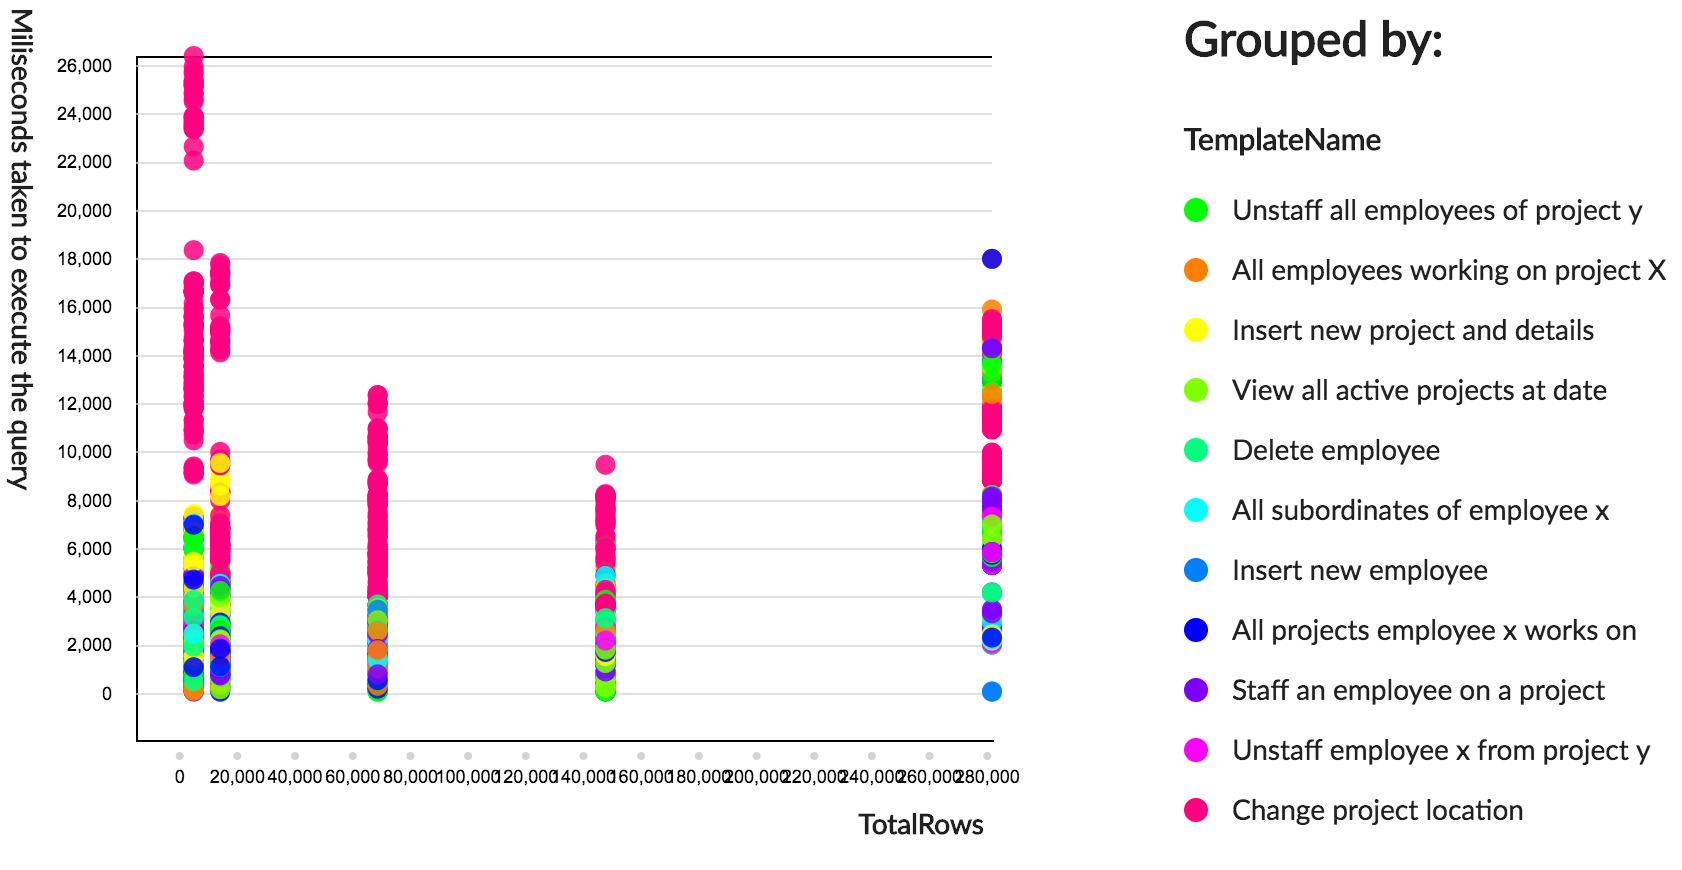
\includegraphics[width=\textwidth]{maria2-temp.png}
		\caption{Using Max Connection Pool as X-axis }
		
	\end{figure}
	\begin{figure}[H]
		\centering
		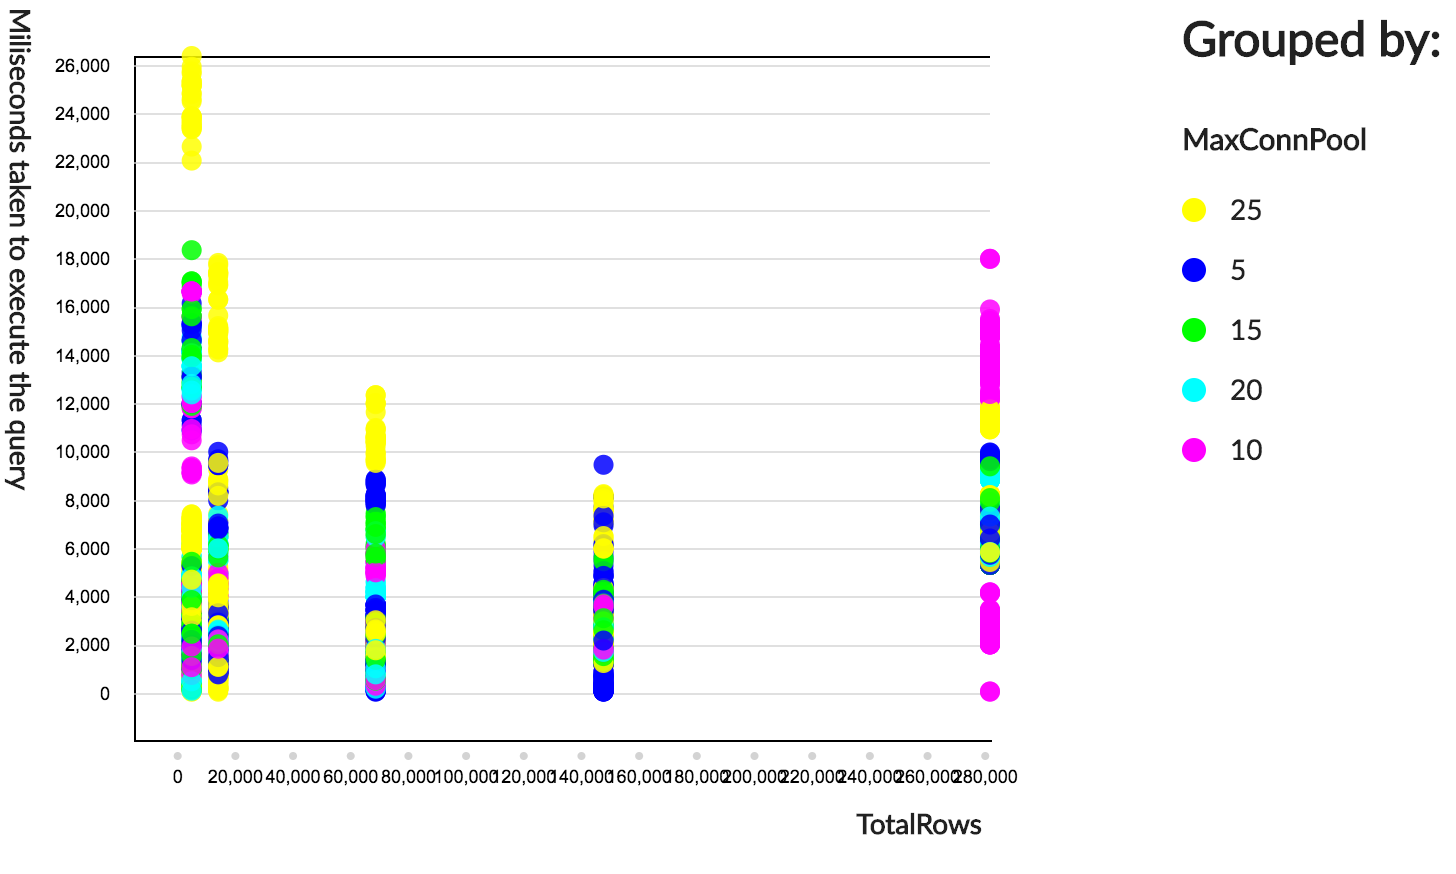
\includegraphics[width=\textwidth]{maria2-conn.png}
		\caption{Using Max Connection Pool as X-axis }
		
	\end{figure}
	\begin{figure}[H]
		\centering
		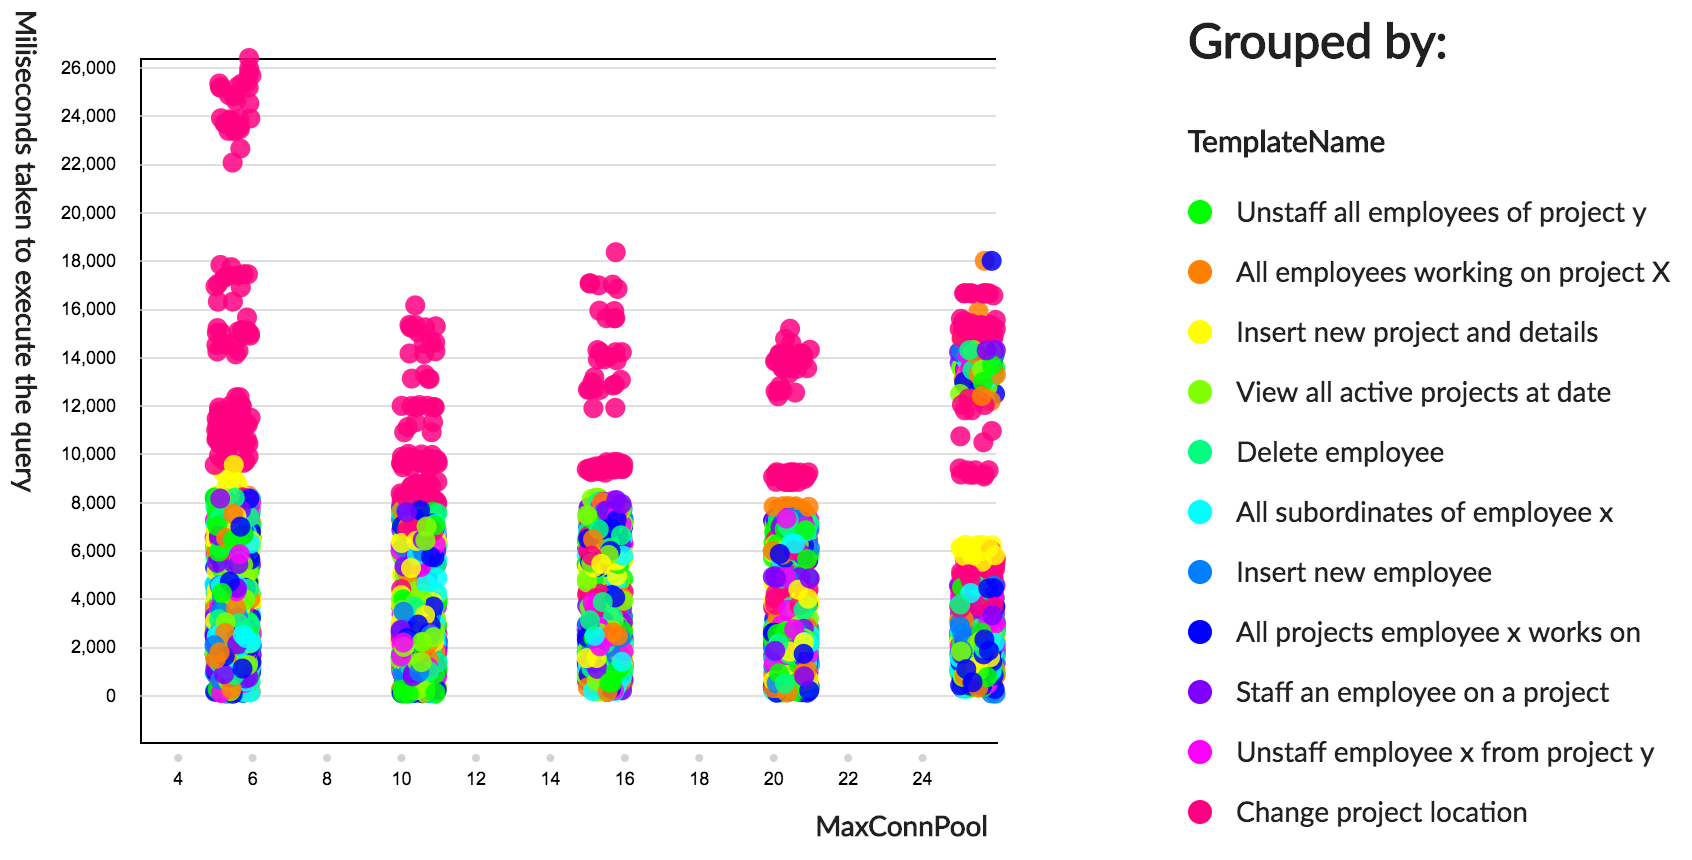
\includegraphics[width=\textwidth]{maria2-mcp.png}
		\caption{Using Max Connection Pool as X-axis }
		
	\end{figure}
	
	
\end{spacing}
\end{document}
